% ******************************* PhD Thesis Template **************************
% Please have a look at the README.md file for info on how to use the template

\documentclass[a4paper,Times,twoside,index,12pt]{Classes/PhDThesisPSnPDF}

% ******************************************************************************
% ******************************* Class Options ********************************
% *********************** See README for more details **************************
% ******************************************************************************

% `a4paper'(The University of Cambridge PhD thesis guidelines recommends a page
% size a4 - default option) or `a5paper': A5 Paper size is also allowed as per
% the Cambridge University Engineering Deparment guidelines for PhD thesis
%
% `11pt' or `12pt'(default): Font Size 10pt is NOT recommended by the University
% guidelines
%
% `oneside' or `twoside'(default): Printing double side (twoside) or single
% side.
%
% `print': Use `print' for print version with appropriate margins and page
% layout. Leaving the options field blank will activate Online version.
%
% `index': For index at the end of the thesis
%
% `draft': For draft mode without loading any images (same as draft in book)
%
% `draftmode': Special draft mode with line numbers, images, and water mark with
% timestamp and custom text. Position of the text can also be modified.
%
% `abstract': To generate only the title page and abstract page with
% dissertation title and name, to submit to the Student Registry
%
% `chapter`: This option enables only the specified chapter and it's references
%  Useful for review and corrections.
%
% ************************* Custom Page Margins ********************************
%
% `custommargin`: Use `custommargin' in options to activate custom page margins,
% which can be defined in the preamble.tex. Custom margin will override
% print/online margin setup.
%
% *********************** Choosing the Fonts in Class Options ******************
%
% `times' : Times font with math support. (The Cambridge University guidelines
% recommend using times)
%
% `fourier': Utopia Font with Fourier Math font (Font has to be installed)
%            It's a free font.
%
% `customfont': Use `customfont' option in the document class and load the
% package in the preamble.tex
%
% default or leave empty: `Latin Modern' font will be loaded.
%
% ********************** Choosing the Bibliography style ***********************
%
% `authoryear': For author-year citation eg., Krishna (2013)
%
% `numbered': (Default Option) For numbered and sorted citation e.g., [1,5,2]
%
% `custombib': Define your own bibliography style in the `preamble.tex' file.
%              `\RequirePackage[square, sort, numbers, authoryear]{natbib}'.
%              This can be also used to load biblatex instead of natbib
%              (See Preamble)
%
% **************************** Choosing the Page Style *************************
%
% `default (leave empty)': For Page Numbers in Header (Left Even, Right Odd) and
% Chapter Name in Header (Right Even) and Section Name (Left Odd). Blank Footer.
%
% `PageStyleI': Chapter Name next & Page Number on Even Side (Left Even).
% Section Name & Page Number in Header on Odd Side (Right Odd). Footer is empty.
%
% `PageStyleII': Chapter Name on Even Side (Left Even) in Header. Section Number
% and Section Name in Header on Odd Side (Right Odd). Page numbering in footer


% ********************************** Preamble **********************************
% Preamble: Contains packages and user-defined commands and settings
\usepackage{lipsum}   % Dummytext
\usepackage{xargs}    % Use more than one optional parameter in a new commands
\usepackage[pdftex,dvipsnames]{xcolor}
\usepackage[colorinlistoftodos,prependcaption,textsize=tiny]{todonotes}

\usepackage{hyperref}
\usepackage{color}


% For french language
\usepackage[french,english]{babel}
\usepackage[utf8]{inputenc}
\usepackage[T1]{fontenc}
\usepackage{lettrine}
\usepackage{aurical}
\usepackage{csquotes}
\usepackage{dirtytalk}


% Package for the content of each chapter
\usepackage{minitoc}


% Package for adding uga cover page
\usepackage{epstopdf}
\usepackage{pdfpages}

%Maths
\usepackage{amsthm}
\usepackage{amssymb}
\usepackage{environ}
\usepackage{mathtools}
\usepackage{amsfonts}
\usepackage{stackrel}
\usepackage{stackengine}
\usepackage{scalerel}
\usepackage{ifthen}
\usepackage{cases}

%spacing
\usepackage{setspace}

%adding description to part
\usepackage{etoolbox}

%Figures

\usepackage{pgfplots}
\usepackage{tikz}
\usepackage{caption}
\usepackage{subfig}
\usetikzlibrary{patterns,intersections,plotmarks,calc,arrows,shapes,snakes,automata,backgrounds,petri,positioning,fit,arrows.meta}
\usepackage{siunitx}


%Font
%\newcommand{\ackfont}{\fontfamily{\Fontskrivan}\selectfont}
\newcommand{\ackfont}{\Fontskrivan}
%Colors
\definecolor{dkgreen}{RGB}{0, 153, 0}
\definecolor{dgreen}{rgb}{.2,.7,.2}

\makeatletter
\let\LaTeXStandardPart\part%
\newcommand{\unstarredpart@@noopt}[1]{%
    \unstarredpart@@opt[#1]{#1}%
}%
    
\newcommand{\unstarredpart@@opt}[2][]{%
  \cleardoublepage% (For clearing content before!!!)
  \begingroup%
  \let\newpage\relax%
  \LaTeXStandardPart[#1]{#2}%
  \endgroup%
}%
                
\newcommand{\starredpart}[1]{%
  \LaTeXStandardPart*{#1}%
}%

\newcommand{\unstarredpart}{%
  \@ifnextchar[{\unstarredpart@@opt}{\unstarredpart@@noopt}%
}%
\renewcommand{\part}{%
  \@ifstar{\starredpart}{\unstarredpart}%
}%of part

%cliquable links
\hypersetup{
colorlinks,
citecolor=black,
filecolor=black,
linkcolor=black,
urlcolor=black
}


%Todo notes: use \listoftodos[Notes] to display all the notes
\newif\ifreview
\reviewtrue
\ifreview
  \newcommandx{\unsure}[2][1=]{\todo[linecolor=red,backgroundcolor=red!25,bordercolor=red,#1]{#2}}
  \newcommandx{\change}[2][1=]{\todo[inline,linecolor=blue,backgroundcolor=blue!25,bordercolor=blue,#1]{#2}}
  \newcommandx{\info}[2][1=]{\todo[linecolor=OliveGreen,backgroundcolor=OliveGreen!25,bordercolor=OliveGreen,#1]{#2}}
  \newcommandx{\improvement}[2][1=]{\todo[linecolor=Plum,backgroundcolor=Plum!25,bordercolor=Plum,#1]{#2}}
\else
  \newcommandx{\unsure}[2][1=]{\todo[disable,linecolor=red,backgroundcolor=red!25,bordercolor=red,#1]{#2}}
  \newcommandx{\change}[2][1=]{\todo[disable,linecolor=blue,backgroundcolor=blue!25,bordercolor=blue,#1]{#2}}
  \newcommandx{\info}[2][1=]{\todo[disable,linecolor=OliveGreen,backgroundcolor=OliveGreen!25,bordercolor=OliveGreen,#1]{#2}}
  \newcommandx{\improvement}[2][1=]{\todo[disable,linecolor=Plum,backgroundcolor=Plum!25,bordercolor=Plum,#1]{#2}}
\fi

%Theorems and definition environment 
\theoremstyle{plain}
\newtheorem{corollary}{Corollary}
\numberwithin{corollary}{section} % important bit

\newtheorem{proposition}{Proposition}
\numberwithin{proposition}{section} % important bit

\newtheorem{theorem}{Theorem}
\numberwithin{theorem}{section} % important bit

\newtheorem{lemma}{Lemma}
\numberwithin{lemma}{section} % important bit

\newtheorem{property}{Property}
\numberwithin{property}{section} % important bit

\theoremstyle{definition}
\newtheorem{definition}{Definition}
\numberwithin{definition}{section} % important bit

\newtheorem{example}{Example}
\numberwithin{example}{section} % important bit

\theoremstyle{remark}
\newtheorem{remark}{Remark}
\numberwithin{remark}{section} % important bit



%TA semantics and predicates
\stackMath
\newcommand{\mf}[1]{\mathbf{#1}}
\newcommand{\mc}[1]{\mathcal{#1}}
\newcommand{\mb}[1]{\mathbb{#1}}
\newcommand{\q}{q} 
\newcommand{\X}{\mc{X}} 
\newcommand{\D}{\mc{D}} 
\newcommand{\E}{\mc{E}} 
\newcommand{\A}{\mc{A}}
\newcommand{\T}{\mc{T}}
\newcommand{\V}{\mc{V}}
\newcommand{\I}{\mc{I}}
\newcommand{\Q}{\mc{Q}} 
\newcommand{\tts}{\texttt{T}}
\newcommand{\TTS}{\tts=(\Q,q_0,\Sigma\cup\mb{K},\to)}
\newcommand{\TTSg}{\tts_g=(\Q_g,q_{0_g},\gamma\cup\realpos,\to_{\gamma})}
\newcommand{\TTSb}[1]{\tts_{#1}=(Q_{#1},q_{0_{#1}},\Sigma\cup\mb{K},\to_{#1})}
\newcommand{\TTSs}{\tts=(\Q,q_0,\A\cup\realpos,\to)}

\newcommand{\TTSbw}[1]{\tts_{#1}=(\Q_{#1},q_{0_{#1}},\Sigma
\cup\{\tau\}\cup\mb{K},\to_{#1})}

\newcommand{\transit}[1]{\xrightarrow{#1}}
\newcommand{\transitb}[2]{\xrightarrow{#1}_{#2}}
\newcommand{\exec}{\varrho}
\newcommand{\texec}{\mf{time(\exec)}}
\newcommand{\integer}{\mb{Z}}
\newcommand{\naturals}{\mb{N}}
\newcommand{\integerpoz}{\mb{Z}_{\ge 0}}
\newcommand{\integerpos}{\mb{Z}_{> 0}}
\newcommand{\realpoz}{\mb{R}_{\ge 0}}
\newcommand{\realpos}{\mb{R}_{> 0}}
\newcommand{\simu}[1]{\sqsubseteq_{#1}}
\newcommand{\simuw}[1]{\dot{\sqsubseteq}_{#1}}
\newcommand{\eqv}[1]{\sim_{#1}}
\newcommand{\eqvw}[1]{\dot{\sim}_{#1}}
\newcommand{\val}{\upsilon}
\newcommand{\Val}{\realpoz^{\X}}
\newcommand{\false}{\textnormal{\textit{false}}}
\newcommand{\true}{\textnormal{\textit{true}}}
\newcommand{\backward}{\raisebox{2pt}{$\swarrow$}}
\newcommand{\backwardp}[2]{\backward^{#2}_{\hspace{-2mm}#1}}
\newcommand{\forward}{\raisebox{2pt}{$\nearrow$}}
\newcommand{\enabledforward}[1]{Enabled\hspace{-0.8pt}\forward\hspace{-1mm}(#1)}
\newcommand{\enabledbackward}[1]{Enabled\hspace{-0.8pt}\backward\hspace{-1mm}(#1)}
\newcommand{\enabledbackwardb}[3]{Enabled\hspace{-0.8pt}\backwardp{#2}{#3}\hspace{-1mm}(#1)}
\newcommand{\Loc}{\mc{L}}
\newcommand{\loc}{\ell}
\newcommand{\locp}{\loc_{\perp}}
\newcommand{\locpb}[2]{\loc_{\perp_{#1}^{#2}}}
\newcommand{\Invb}[2]{\I_{#1}(#2)}
\newcommand{\Inv}[1]{\I(#1)}
\newcommand{\tc}{B=(\Loc,\loc_0,\X,\A,\E,\I)}
\newcommand{\tci}[1]{B_{#1}=(\Loc_{#1},\loc_{0_{#1}},\X_{#1},\A_{#1},\E_{#1},\I_{#1})}
\newcommand{\enabled}[1]{Enabled(#1)}
\newcommand{\p}[1]{part(#1)}
\newcommand{\urgent}{Urgent}
\newcommand{\al}[1]{\textsf{at}(#1)}
\newcommand{\action}{\textsf{action}}
\newcommand{\source}{\textsf{source}}
\newcommand{\target}{\textsf{target}}
\newcommand{\guard}{\textsf{guard}}
\newcommand{\reset}{\textsf{reset}}
%\newcommand{\hmn}{h_{\min}}
\newcommand{\reacha}[1]{\overline{Reach(#1)}}
%\newcommand{\stacktxt}[1]{\mathit{\stackon[0pt]{#1}{\hstretch{7.0}{\sim}}}}
\newcommand{\lpsabrb}{LPS }
\newcommand{\lpsabr}{LPS}
\newcommand{\lps}{local planning semantics }
\newcommand{\lpsb}{local planning semantics}
\NewEnviron{myequation}{%
\begin{displaymath}
\scalebox{1.5}{$\BODY$}
\end{displaymath}
}


%%%%%%%%%%%%%%%%%%PLANNING%%%%%%%%%%%%%%%%%%%%%%%%%%%%%%%%
\newcommand{\squig}{{\scriptstyle\sim\mkern-3.9mu}}
\newcommand{\lsquigend}{{\lhd\mkern-3mu}}
\newcommand{\rsquigend}{{\scriptstyle\rule{.1ex}{0ex}>}}
\newcounter{sqindex}
\newcommand\squigs[1]{
    \setcounter{sqindex}{0}
      \whiledo {\value{sqindex}< #1}{\addtocounter{sqindex}{1}\squig}
    }
\newcommand{\tranbp}[2]{
  \mathbin{\stackon[2pt]{\squigs{#2}\rsquigend}{\scriptstyle{#1\,}}}_{\gamma}
}

 
\makeatletter
\def\namedlabel#1#2{\begingroup
  \mbox{\hspace{1cm}}#2%
    \def\@currentlabel{#2}%
    \phantomsection\label{#1}\endgroup
}
\makeatother

\makeatletter
\newcommand{\mytag}[2]{%
 \text{#1}%
  \@bsphack
    \protected@write\@auxout{}%
   {\string\newlabel{#2}{{#1}{\thepage}}}%
  \@esphack
}          
\makeatother


\newcommand{\confl}{\mathit{conf}}
\newcommand{\pmin}{\min(\pi)}
\newcommand{\hmin}{h_{\min}}
\newcommand{\hmax}{h_{\max}}
\newcommand{\hmaxt}{h_{\max}^{\infty}}
\newcommand{\hmaxm}{h_{\max}^{\hmin}}
\newcommand{\hmxb}[1]{h_{\max}(#1)}
\newcommand{\hmx}{h_{\max}(\alpha)}
\newcommand{\plntxt}[1]{\mathit{Plannable(#1)}}
\newcommand{\plntxtb}[1]{\mathit{\stackon[0pt]{Plannable(#1)}{\hstretch{7.0}{\sim}}}}


\newcommand{\tcal}[1]{\mathcal{#1}}
\newcommand{\lto}{\longrightarrow}
\newcommand{\urgb}{\tsf{urg}}
\newcommand{\urg}{\textnormal{\textit{urg}}}
\newcommand{\tpcp}[1]{\textsf{tpc}(#1)}
\newcommand{\tpc}{\textsf{tpc}}

\newcommand{\pln}[1]{\mathit{Plannable(#1)}=\bigvee_{\loc\in\Loc_{#1}}
\al{\loc}\wedge\backhtxt(\bigwedge_{a_i\in#1} \guard{a_i}{\loc_i})}

\newcommand{\plnIntxt}[2]{\mathit{Plannable(#1,#2)}}
\newcommand{\plnIn}[2]{\mathit{Plannable(#1,#2)}=\bigvee_{\loc\in\Loc_{#1}}
\al{\loc}\wedge\bigwedge_{a_i\in#1} \Big(\guard{a_i}{\loc_i}+#2\Big)}
%%%%%%%%%%%%%%%%%%%%%%%%%%%%%%%%%%%%%%%%%%%%%%%%%%%%%%%%%%%%%%%%%%%%%%%%%%



\newcommand{\clock}[1]{\textsf{clock}(#1)}

\newcommand{\valdt}{v^{dt}}                              % valuation of the clocks
\newcommand{\valdtb}{v^{dt'}}                              % valuation of the clocks
\newcommand{\valg}{\bar{v}}                              % valuation of the clocks
\newcommand{\valgp}{\bar{v'}}  
\newcommand{\qdt}{q^{dt}}
\newcommand{\qdtb}{q^{dt'}}
\newcommand{\RS}{R}
\newcommand{\enabledb}{\mathit{Enabled}^{{\scriptscriptstyle
\swarrow^{\epsilon}}}}
\newcommand{\enabledf}{\mathit{Enabled}^{{\scriptscriptstyle
\nearrow^{\epsilon}}}}
\newcommand{\reach}{\textit{Reach}}
\newcommand{\simdt}{\sqsubseteq^{\epsilon*}_{\RS}}

%%%%%%%%%%%%%%%%%%%%%%%%%%%%%%%%%%%%%%%%%%%%DRIFT%%%%%%%%%%%%%%%%%%%%%%%%%%%
\makeatletter
\pgfdeclareshape{document}{
\inheritsavedanchors[from=rectangle] % this is nearly a rectangle
\inheritanchorborder[from=rectangle]
\inheritanchor[from=rectangle]{center}
\inheritanchor[from=rectangle]{north}
\inheritanchor[from=rectangle]{south}
\inheritanchor[from=rectangle]{west}
\inheritanchor[from=rectangle]{east}
\inheritanchor[from=rectangle]{north east}
\inheritanchor[from=rectangle]{north west}
\inheritanchor[from=rectangle]{south east}
\inheritanchor[from=rectangle]{south west}
% ... and possibly more
\backgroundpath{% this is new
% store lower right in xa/ya and upper right in xb/yb
\southwest \pgf@xa=\pgf@x \pgf@ya=\pgf@y
\northeast \pgf@xb=\pgf@x \pgf@yb=\pgf@y
% compute corner of ‘‘flipped page’’
\pgf@xc=\pgf@xb \advance\pgf@xc by-7pt % this should be a parameter
\pgf@yc=\pgf@yb \advance\pgf@yc by-7pt
% construct main path
\pgfpathmoveto{\pgfpoint{\pgf@xa}{\pgf@ya}}
\pgfpathlineto{\pgfpoint{\pgf@xa}{\pgf@yb}}
\pgfpathlineto{\pgfpoint{\pgf@xc}{\pgf@yb}}
\pgfpathlineto{\pgfpoint{\pgf@xb}{\pgf@yc}}
\pgfpathlineto{\pgfpoint{\pgf@xb}{\pgf@ya}}
\pgfpathclose
% add little corner
\pgfpathmoveto{\pgfpoint{\pgf@xc}{\pgf@yb}}
\pgfpathlineto{\pgfpoint{\pgf@xc}{\pgf@yc}}
\pgfpathlineto{\pgfpoint{\pgf@xb}{\pgf@yc}}
\pgfpathlineto{\pgfpoint{\pgf@xc}{\pgf@yc}}
}
}
\makeatother


\tikzstyle{doc}=[%
  draw,
  thick,
  align=center,
  color=black,
  shape=document,
  minimum width=11mm,
  minimum height=6mm,
  shape=document,
  inner sep=1ex,
]


\tikzset{                                 
  connect/.style args={(#1) to (#2) over (#3) by #4}{
    insert path={                         
    let                             
    \p1=($(#1)-(#3)$),            
    \n1={veclen(\x1,\y1)},        
    \n2={atan2(\y1,\x1)},         
    \n3={abs(#4)},                
    \n4={#4>0 ?180:-180}          
      in                            
      (#1) -- ($(#1)!\n1-\n3!(#3)$) 
      arc (\n2:\n2+\n4:\n3) -- (#2) 
    }                                     
  },                                       
  rc/.style={rounded corners=2mm,line width=1pt},
  ->,
  node distance=1.3cm,
  >=stealth',
  bend angle=20,
  auto,
  place/.style={text width=6mm,align=center,circle,thick,draw=blue!75,fill=blue!20,minimum size=8mm},
  redplace/.style={place,draw=red!75,fill=red!20},
  markplace/.style={place,draw=black!75,fill=black!20},
  dots/.style={fill=black,circle,inner sep=2pt},
  initial text={},
  sh2w/.style={shift={(-0.7,0)}},
  sh2w2/.style={shift={(-1.5,0)}},
  sh2nw/.style={shift={(-0.7,0.5)}},
  sh2ne/.style={shift={(0.7,0.5)}},
  sh2sw/.style={shift={(-0.7,-0.5)}},
  sh2sw2/.style={shift={(-1.5,-0.5)}},
  sh2se/.style={shift={(0.7,-0.5)}},
  h2n/.style={shift={(0,.5)}},
  h2s/.style={shift={(0,-.5)}},
  h2se/.style={shift={(0.5,-1.1)}},
  h2e/.style={shift={(0.5,0)}},
  rc/.style={rounded corners=2mm},
  triangle/.style={fill=black,regular polygon,regular polygon sides=3,
   minimum size=10pt,inner sep=0pt},
  transition/.style={
    rectangle,
    thick,
    fill=black,
    minimum width=7mm,
    inner ysep=0.5mm
  },
  rectnodes/.style args={#1,#2}{
  draw=black,        
  rounded corners,
  thick,             
  minimum width=#1 cm,
  minimum height=#2 cm,
  },                   
  rectnode/.style args={#1,#2}{
  rounded corners,
  draw=red!50,       
  fill=yellow!30,    
  thick,             
  minimum width=#1 cm,
  minimum height=#2 cm,
  }        
}       

\definecolor{mymagenta}{RGB}{226,0,116}
\definecolor{mygray}{RGB}{208,208,208}
\newcommand*{\mytextstyle}{\color{black}}
\newcommand{\arcarrow}[4]{%
   % inner radius, middle radius, outer radius, start angle,
   % end angle, tip protusion angle, options, text
   \pgfmathsetmacro{\rin}{3}
   \pgfmathsetmacro{\rmid}{3.5}
   \pgfmathsetmacro{\rout}{4}
   \pgfmathsetmacro{\astart}{#1}
   \pgfmathsetmacro{\aend}{#2}
   \pgfmathsetmacro{\atip}{1}
   \fill[#4, very thick] (\astart+\atip:\rin)
                         arc (\astart+\atip:\aend:\rin)
      -- (\aend-\atip:\rmid)
      -- (\aend:\rout)   arc (\aend:\astart+\atip:\rout)
      -- (\astart:\rmid) -- cycle;
   \path[
      decoration = {
         text along path,
         text = {|\mytextstyle|#3},
         text align = {align = center},
         raise = -1.0ex
      },
      decorate
   ](\astart+\atip:\rmid) arc (\astart+\atip:\aend+\atip:\rmid);
}



%\addbibresource{References/references.bib}
% ************************ Thesis Information & Meta-data **********************
% Thesis title and author information, refernce file for biblatex
% ************************ Thesis Information & Meta-data **********************
%% The title of the thesis
\crest{
\includegraphics[scale=0.15]{uga}}
\title{Formal Methods for Distributed Real-Time Systems}
%\title{Writing your PhD thesis in \texorpdfstring{\\ \LaTeX2e}{LaTeX2e}}
%\texorpdfstring is used for PDF metadata. Usage:
%\texorpdfstring{LaTeX_Version}{PDF Version (non-latex)} eg.,
%\texorpdfstring{$sigma$}{sigma}

%% Subtitle (Optional)
%\subtitle{Using the CUED template}

%% The full name of the author
\author{Dellabani Mahieddine}

%% Department (eg. Department of Engineering, Maths, Physics)
\dept{Laboratoire Verimag}

%% University and Crest
\university{Université Grenoble Alpes}

%% You can redefine the submission text:
% Default as per the University guidelines:
% ``This dissertation is submitted for the degree of''
%\renewcommand{\submissiontext}{change the default text here if needed}

%% Full title of the Degree
\degree{Doctor of Philosophy}

%% College affiliation (optional)
\college{Ecole Doctorale Mathématique, Sciences et Technologies de
l’Information, Informatique (MSTII)}
%% Submission date
% Default is set as {\monthname[\the\month]\space\the\year}
%\degreedate{September 2014} 

%% Meta information
%\subject{LaTeX} \keywords{{LaTeX} {PhD Thesis} {Engineering} {University of
%Cambridge}}

\listfiles

% ***************************** Abstract Separate ******************************
% To printout only the titlepage and the abstract with the PhD title and the
% author name for submission to the Student Registry, use the `abstract' option in
% the document class.

\ifdefineAbstract
 \pagestyle{empty}
 \includeonly{Declaration/declaration, Abstract/abstract}
\fi

% ***************************** Chapter Mode ***********************************
% The chapter mode allows user to only print particular chapters with references
% Title, Contents, Frontmatter are disabled by default
% Useful option to review a particular chapter or to send it to supervisior.
% To use choose `chapter' option in the document class

\ifdefineChapter
 \includeonly{Chapter3/chapter3}
\fi


% ***************************** Minitoc Settings ********************************

\setcounter{minitocdepth}{2} 
\setlength{\mtcindent}{24pt} 
\renewcommand{\mtcfont}{\small\rm} 
\renewcommand{\mtcSfont}{\small\bf} 

\nobibliography*
% ******************************** Front Matter ********************************
\begin{document}

\frontmatter

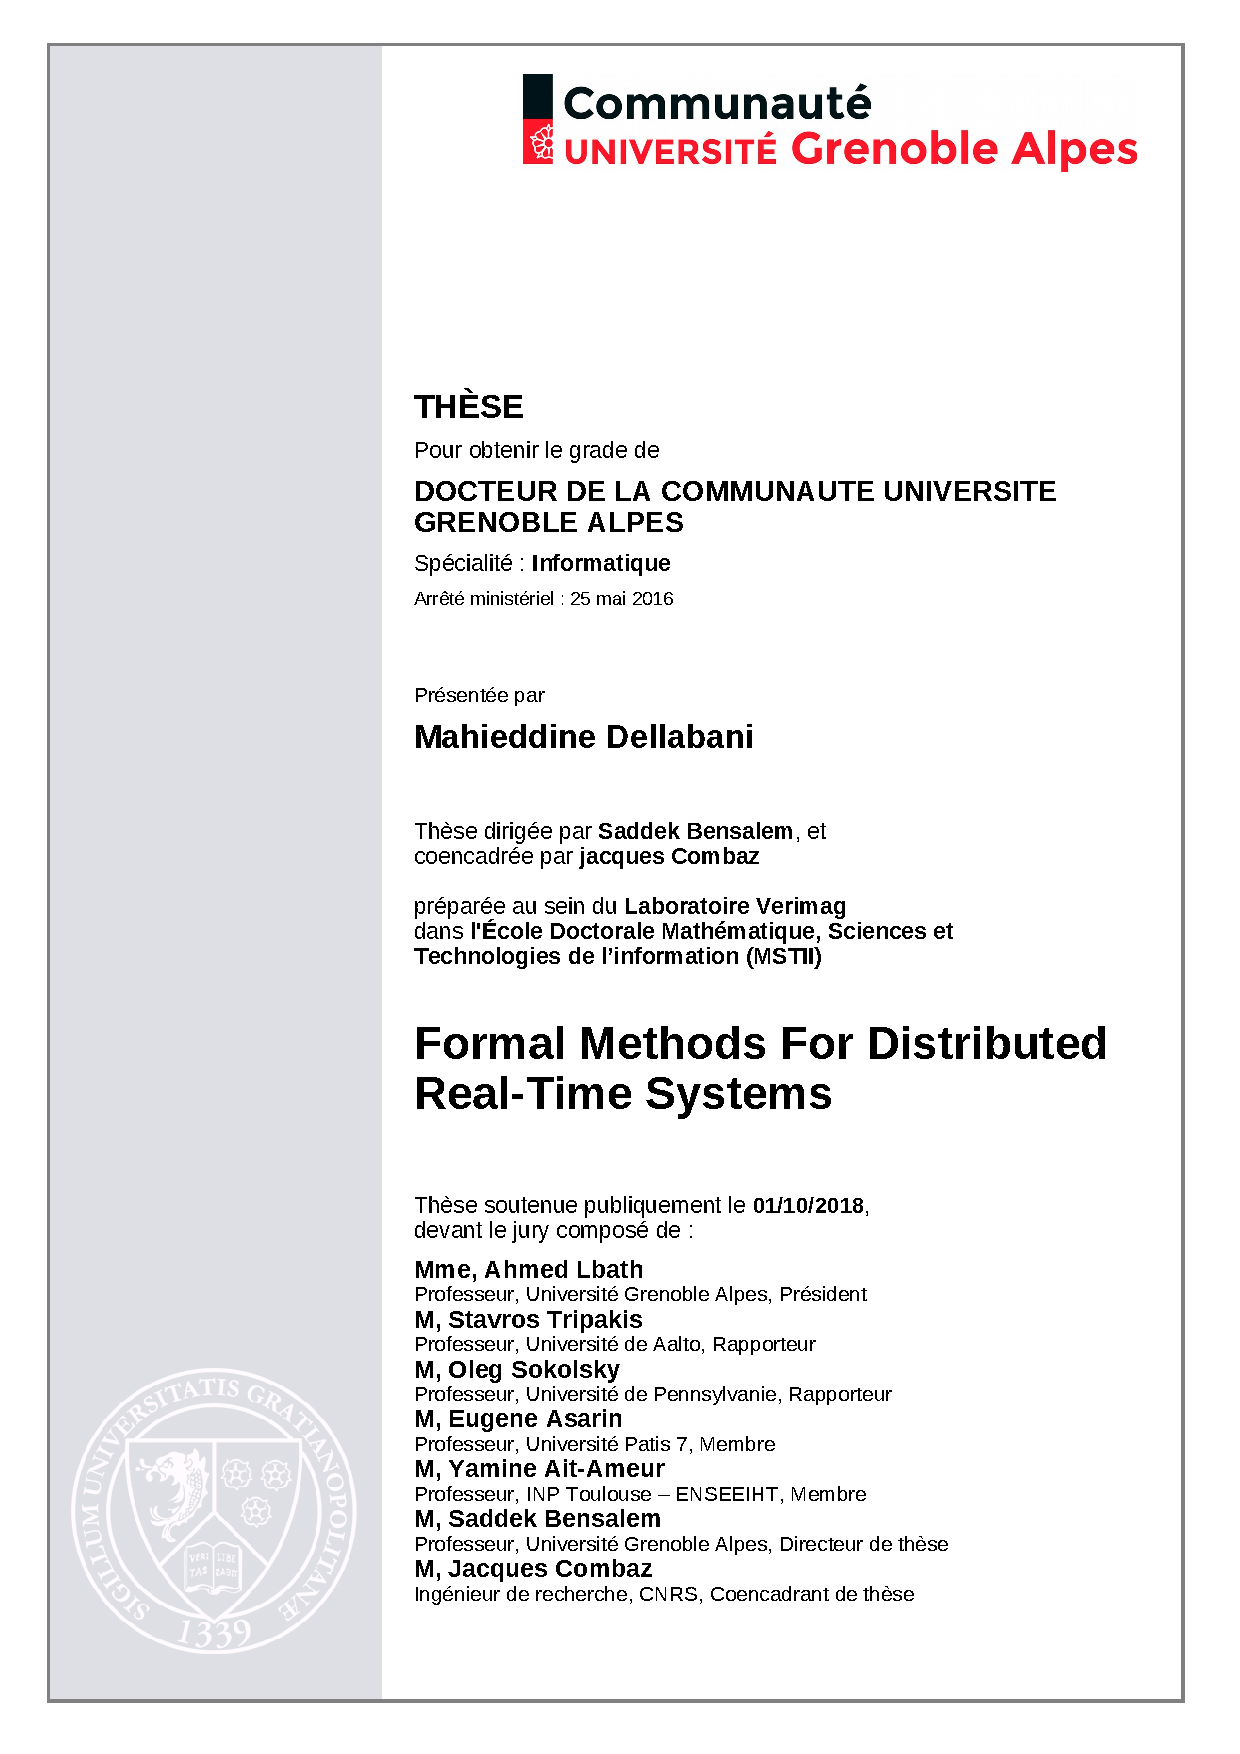
\includepdf[pages=-]{cover.pdf}


\begin{titlepage}
  \maketitle
\end{titlepage}

\mainmatter

%\include{Dedication/dedication}
%\include{Declaration/declaration}
\begin{acknowledgements}
\begin{otherlanguage}{french}
\ackfont
\lettrine[lines=4]{\color{BrickRed}S}{tart} of the chapter
trrrrrrrrrrrrrrrrrrrrrrrrrrrrrrrrrrrrrrrrr
rrrrrrrrrrrrrrrrrrrrrr
\end{otherlanguage}
\end{acknowledgements}


\begin{abstract}


Nowadays, real-time systems are ubiquitous in several application domains. 
Such an emergence led to an increasing need of performance (resources, 
availability, concurrency, etc) and initiated a shift from the
use of single processor based hardware platforms, to large sets 
of interconnected and distributed computing nodes. This trend introduced the birth 
of a new family of systems known as \emph{Networked Embedded Systems}, 
that are intrinsically distributed.
Such an evolution stems from the growing complexity of real-time software 
embedded on such platforms (e.g. electronic control in avionics 
and automotive domains), and the need to integrate formerly isolated systems so that 
they can cooperate, as well as, share resources improving thus functionality 
and reducing costs.
Undoubtedly, the design, implementation and verification of such systems are 
acknowledged to be very hard tasks since they are
are prone to different kinds of factors 
that increases considerably the complexity of coordinating parallel activities.
  %recurrent in suchlike applications. 

In this thesis, we propose a rigorous design flow that addresses part of the aspects that
needs to be considered when building distributed real-time applications.
We investigate formal timed automata based models, with well defined semantics, in order 
to study the behavior of a given system with some imposed timing constraints when deployed 
in a distributed environment. Particularly, we study \emph{(i)} the impact of the communication 
delays by introducing a minimum latency between actions execution and their effective 
scheduling date, and \emph{(ii)} the effect of hardware imperfections, more precisely clock 
drifts, on systems execution by breaking the synchrony hypothesis, often adopted during 
the modeling phase. Nevertheless, timed automata formalism is intended to describe a high
level abstraction of the behavior of a given application, free from the physical constraints of
the its deployment environment. Therefore, we use an intermediate representation of 
the initial application, that besides having \say{equivalent} behavior, explicitly expresses
implementation mechanism, and thus reduce the gap between the modeling and the concrete
implementation. Additionally,  we contribute in building such models by \emph{(iii)} 
proposing a knowledge based optimization that aims to eliminate unnecessary computation time 
or exchange of messages during execution. 
  
We compare the behavior of each proposed model to the initial high level model and study the
relationships between both. Then, we identify and formally characterize the potential problems 
resulting from these additional constraints and propose execution strategies that allows
to preserve some desired properties and achieve a \say{similar} execution scenario, faithfull
to the original specifications.   
  
\end{abstract}


\begin{abstractfr}
\end{abstractfr}


% *********************** Adding TOC and List of Figures ***********************

\dominitoc
\dominilof
\dominilot
\renewcommand{\baselinestretch}{0.9}\normalsize
\tableofcontents
\renewcommand{\baselinestretch}{1.0}\normalsize
%\tableofcontents

%\listoffigures\mtcaddchapter 

%\listoftables\mtcaddchapter 
\adjustmtc
% \printnomencl[space] space can be set as 2em between symbol and description
%\printnomencl[3em]

%\printnomencl

% ******************************** Main Matter *********************************
\chapter{Introduction}
\section{Distributed Real-Time Systems}
\section{From Modelling to Implementation of Distributed Real-Time Systems}
\subsection{Modeling}
\subsection{Implementation}
\subsection{Validation}
\section{Contribution and Organization}

\part{Preliminaries}
{\label{part:1}
  In this part, we give formal definitions and present results that will be used in subsequent
chapters. Chapter~\ref{chap:2} provides formal definitions of timed transition systems,
timed automata, their semantics and properties, as well as a variant of the latter.
It also discusses the verification technique used in this thesis. Chapter~\ref{chap:3}
explains how an intermediate representation based on the timed automata formalism
can be used to represent a realistic view of a distributed real-time systems. It also tackles
two important constraints that an application can incur when being deployed in a distributed
environment under real-time restriction.} 
%\chapter{Timed Systems and Semantics}\label{chap:2} 
\minitoc
\section{Timed Transition Systems}
Transition systems provide a general and convenient method for modeling 
systems and have been used frequently to model the behavior of 
software and hardware systems. They define graphs where nodes
represent the possible \emph{states} of the system, and edges model 
\emph{transitions}, that is, state changes. A state encodes all the relevant 
information at a certain instant, whereas a transition describes how the system
evolves between two states. 

Nowadays, several variants of transition system formalisms have been 
proposed. For instance, a labeled transition system is a transition system
where the set of transitions is labeled by \emph{actions}.
In this thesis, we use \emph{Timed Transition Systems} (TTS)
to explicitly model the effect of time passage (besides the actions)
on the states of the system. Formally, it is defined as follows:  

\begin{definition}[Timed Transition System]\label{def:tts}
  A timed transition system is a tuple $\TTS$ such that $\mc{Q}$ is 
  a set of states, $q_0\in\mc{Q}$ is the initial state, $\Sigma$ is a set of
  actions, $\mb{K}$ is a time domain and $\to\subseteq\mc{Q}\times
  (\Sigma\cup\mb{K})\times\mc{Q}$ is the transition relation.
\end{definition}
Consequently, we distinguish two types of transition:
\begin{itemize}
  \item \emph{action step} $\transit{\sigma}$ for $\sigma\in\Sigma$ and we write 
    $q\transit{\sigma}q'$. 
  \item \emph{time step} $\transit{d}$ for $d\in\mb{K}$ and we write $q\transit{d}q'$. 
\end{itemize}
We write $q\transit{d,\sigma}q''$ if there exists $q'\in\mc{Q}$
such that $q\transit{d}q'\transit{\sigma}q''$. We say that $q'$ is
a time successor of $q$.

Given a TTS $\TTS$, a \emph{run} $\exec$ of $\tts$ (also called 
\emph{execution sequence}), is a path that alternates action steps and 
time steps, that is:
\begin{displaymath}
  \exec=s_0\sigma_0 s_1\sigma_1 s_2\cdots \text{ such that } 
  s_i\in\mc{Q}, \  s_i\transit{\sigma_{i}}s_{i+1},\text{ and } 
  i\in\integerpoz,\sigma_i\in\Sigma\cup\mb{K}
\end{displaymath}

We denote by $\texeci$ the total elapsed time until point $i$, that is,
$\sum_{j<i}\sigma_j$ such as $\sigma_j\in\mb{K}$. In the same way, $\texec$ represents
the total elapsed time during $\varrho$, and is defined to be the limit of $\texeci$
if the sequence converges and $\infty$ otherwise.
A run $\exec$ is said to be an \emph{initial run} if $s_0=q_0$. 

A state $q\in\mc{Q}$ is called reachable if there exists an initial run
that leads to state $q$. We put $Reach(\tts)$ to denote the set of all 
reachable states of $\tts$.
\subsection{Comparing Timed Transition Systems}
In this thesis, we use the concept of (bi)simulation~\cite{bsim} 
in order to attest the similarity of timed transition systems.
\begin{definition}[Simulation]\label{def:sim}
  Given two TTS $\TTSb{1}$ and $\TTSb{2}$, a simulation relation from 
  $\ttsb{1}$ to $\ttsb{2}$ is a binary relation $\mc{R}\subseteq\mc{Q}_1
  \times\mc{Q}_2$ such that:
  \begin{itemize}
    \item $\forall(q_1,q_2)\in\mc{R},\forall\sigma\in\Sigma,\ 
      q_1\transitb{\sigma}{1}q_1'\Rightarrow\exists q'_2\in\mc{Q}_2 
      \text{ such that } q_2\transitb{\sigma}{2}q_2'\wedge
      (q_1',q_2')\in\mc{R}$
    \item $\forall(q_1,q_2)\in\mc{R},\forall d\in\mb{K},\ 
      q_1\transitb{d}{1}q_1'\Rightarrow\exists q'_2\in\mc{Q}_2 
      \text{ such that } q_2\transitb{d}{2}q_2'\wedge
      (q_1',q_2')\in\mc{R}$
  \end{itemize}
\end{definition}
  $\ttsb{2}$ simulates $\ttsb{1}$, denoted by $\ttsb{1}\simu{\mc{R}}\ttsb{2}$
  means that $\ttsb{2}$ can do everything $\ttsb{1}$ does. Notice that if
  $\ttsb{1}\simu{\mc{R}}\ttsb{2}$ and $\ttsb{2}\simu{\mc{R}}\ttsb{1}$,
  we say that $\ttsb{1}$ and $\ttsb{2}$ are bisimilar, denoted by
  $\ttsb{1}\eqv{\mc{R}}\ttsb{2}$.  

In some cases, this notion of simulation is refined in order to consider only
a part of a system behavior. This is usually the case when a system
performs \emph{internal} (or \emph{silent}) actions not visible by external
observers. This variant of simulation is called \emph{weak simulation}.

\begin{definition}[Weak Simulation]\label{def:wsim}
  Given two TTS $\TTSbw{1}$ and $\TTSbw{2}$, where $\tau$ actions 
  represent silent (unobservable) actions, a weak simulation relation from 
  $\ttsb{1}$ to $\ttsb{2}$, denoted $\ttsb{1}\simuw{\mc{R}}\ttsb{2}$, 
  is a binary relation $\mc{R}\subseteq\mc{Q}_1
  \times\mc{Q}_2$ such that:
  \begin{itemize}
    \item $\forall(q_1,q_2)\in\mc{R},\ 
      q_1\transitb{\tau}{1}q_1'\Rightarrow\exists q'_2\in\mc{Q}_2 
      \text{ such that } q_2\transitb{\tau^*}{2}q_2'\wedge
      (q_1',q_2')\in\mc{R}$
    \item $\forall(q_1,q_2)\in\mc{R},\forall\sigma\in\Sigma,\ 
      q_1\transitb{\sigma}{1}q_1'\Rightarrow\exists q'_2\in\mc{Q}_2 
      \text{ such that } q_2\transitb{\tau^*\sigma\tau^*}{2}q_2'\wedge
      (q_1',q_2')\in\mc{R}$
    \item $\forall(q_1,q_2)\in\mc{R},\forall d\in\mb{K},\ 
      q_1\transitb{d}{1}q_1'\Rightarrow\exists q'_2\in\mc{Q}_2 
      \text{ such that } q_2\transitb{\tau^*d\tau^*}{2}q_2'\wedge
      (q_1',q_2')\in\mc{R}$
  \end{itemize}
\end{definition}
  We say that $\ttsb{1}$ and $\ttsb{2}$ are observationally equivalent,
  denoted $\ttsb{1}\eqvw{\mc{R}}\ttsb{2}$ , if it exists a weak simulation 
  from $\ttsb{1}$ to $\ttsb{2}$ and vice versa.
  
  In chapter~\ref{chap:6}, we will introduce an even weaker notion of simulation 
  that characterizes the degree of closeness (in term of delays)
  between two timed systems. 

\subsection{Reactive Timed Systems}
Reactive systems are supposed to execute forever, that is,
they are supposed to act infinitely often. We refer to this characteristic as 
the \emph{requirement of progress}~\cite{progress}. 
Particularly, a timed system evolves either through an action step or 
by letting the time pass (time step).
This evolution imposes thus two requirements of progress:
discrete progress (resp. time progress) meaning that a timed system
should be able to perform action steps (resp. time steps) infinitely
often. In the physical world however, no matter how fast a system can
evolve, it cannot be infinitely fast. This induces the following constraints
on the progress of time:
\begin{enumerate}
  \item Only a finite number of actions can happen in a certain amount of time
  \item Only a bounded number of actions can happen in zero time
\end{enumerate}

\subsubsection{Time Progress (Zeno runs \& Timelocks)} 
We distinguish two types of anomalies that infringe the time progress in
a timed system namely \emph{zeno} runs and \emph{timelocks}.
A run $\exec$ is called \emph{zeno} if it is 
an infinite run and if $\texec\neq\infty$. Such a run transgresses the 
first point of the time progress presented above.
Timelocks are states from which all infinite runs starting from these states
are zeno.
\subsubsection{Discrete Progress (Deadlocks)}
States violating the discrete progress are called \emph{deadlock} states.
Formally, a state is said to be deadlock if no action can be executed from 
that state nor from any of its time successors. 

Any model of a reactive timed system should properly capture the behavior 
of the latter. Particularly, the corresponding model must react infinitely often,
that is, it must not block time or execute an unbounded number of actions in zero 
time. In that sense, we can say that deadlocks and timelocks are modeling errors
that needs to be cleared, either during the modeling process (which is tedious 
for large scale systems) or by providing verification methods that guarantee
their absence. 


\section{Timed Systems Syntax and Semantics}\label{sec:2.2}
\subsection*{Clocks}
In order to represent and measure the dense time domain, we rely on positive 
real valued variables, the \emph{clocks}. Clocks are 
positive real variables increasing synchronously (with the same rate) in a 
given system. They are used to express the progress of time and impose 
a certain dynamic on the execution of a timed system.

Given a finite set of clocks $\mc{X}$, we define the valuation function
$\val:\mc{X}\to\realpoz$ assigning to each clock $x$ a positive real value 
$\val(x)$. We put $\Val$ to denote the set of all valuations.
For a valuation $\val\in\Val$ and $d\in\realpoz$, $\val+d$ is the valuation
satisfying $(\val+d)(x)=\val(x)+d$, while for a subset of clocks 
$r\subseteq\mc{X}$, $\val[r]$ is the valuation obtained from $\val$ by 
resetting clocks of $r$, that is, $\val[r](x)=0$ for $x\in r$ and
$\val[r](x)=\val(x)$ otherwise. We write {\bf 0} for the valuation 
that assigns 0 to every clock.

An \emph{atomic clock constraint} is an expression of the form:
\begin{displaymath}
  c:=\true \ | \ x\#k \ |\ x-y\#k \
\end{displaymath}
where $x$ and $y$ are clocks in $\mc{X}$, $\#\in\{<,\le,=,\ge,>\}$,
and $k\in\integer$. A clock constraint is a conjunction of atomic clock 
constraint, that is:
\begin{equation}\label{eq:cc}
  c:=\true \ | \ x\#k \ |\ x-y\#k \ | \ c_1\wedge c_2 
\end{equation}
with $c_1$ and $c_2$ being atomic clock constraints. We write $\mc{C(X)}$
for the set of clock constraints over $\mc{X}$.
Given a clock constraint $c$ and a valuation $\val$, we say that $\val$
satisfies $c$, denoted $\val\models c$, if all constraints are satisfied
when each $x\in\mc{X}$ is replaced by $\val(x)$. 
We also consider for a clock constraint $c$ the classical \emph{backward} 
and \emph{forward} operators on
clock constraints:
\begin{align*}
  &\text{ \bf Backward } &:& \val\models\backward c\Leftrightarrow 
  \exists d\in\realpoz.\ \val+d\models c\\ 
  &\text{ \bf Forward } &:& \val\models\forward c\Leftrightarrow 
  \exists d\in\realpoz.\ \val-d\models c\\ 
\end{align*}

Additionally, we also use another variant of the backward operator considering
lower bounds $l\in\integerpoz$ and upper bounds $u\in\integerpoz\cup
\{+\infty\}$:

\begin{displaymath}
  \val\models\backwardp{l}{u} c\Leftrightarrow 
  \exists d\in\realpoz, l\le d\le u. \ \val+d\models c\\ 
\end{displaymath}

\subsection{Timed Components Syntax and Semantics}
In this thesis, components are timed automata and systems are compositions of timed automata
with respect to multiparty interactions. The timed automata we use are essentially the ones from
~\cite{AlurD94}, however, slightly adapted to embrace a uniform notation the dissertation.
\begin{definition}[Timed Component]\label{def:tc}
  A component is a tuple $B=(\Loc,\loc_0,\X,\A,\E,\I)$, where:
  \begin{itemize}
    \item $\Loc$ is a finite set of locations, with $\loc_0\in\Loc$ is the 
      initial location,
    \item $\mc{X}$ is a finite set of clocks,
    \item $\mc{A}$ is a finite set of actions
    \item $\mc{E}\subseteq\Loc\times(\mc{A}\times\mc{C(X)}\times2^{\mc{X}})
      \times\Loc$ is a finite set of transitions labeled with an action, 
      a clock constraint (guard), and a set of clocks to be reset,
    \item $\mc{I}:\Loc\to\mc{C(X)}$ is the function assigning an invariant
      to each location. Notice that invariants are restricted to conjunction
      of atomic clock constraints of the form $x\le k$. 
  \end{itemize}
\end{definition}

Throughout this thesis, we consider 
\emph{deterministic} timed components, that is, at a given location
$\loc$ and for a given action $a$, there is up to one outgoing transition
from $\loc$ labeled by a. 
A transition $e=(\loc,(a,g,r),\loc')\in\mc{E}$ is also denoted by
$\loc\transit{a,g,r}\loc'$. We write $\source(e)$, $\target(e)$, $\action(e)$, $\guard(e)$
and $\reset(e)$ for $\loc$, $\loc'$, $a$, $g$ and $r$, respectively.
We also denote by $\Phi(a,\loc)$ the guard 
of the transition labeled by $a$ and outgoing from $\loc$
if it exists, and $\false$ otherwise. It is formalized as follows:
\[\Phi(a,\loc)=\begin{cases}
  g,& \text{ if } \exists e=(\loc,a,g,r,\loc')\in\mc{E}  \\
  \false,& otherwise
\end{cases}\]

\begin{example}
  Figure~\ref{fig:tc} depicts a timed component $B$ where locations
  are represented by circles and transitions are the directed arrows
  from a location to another. The initial location ($\loc_0$ here) is
  represented by a double circle. The component 
  $B=(\Loc,\loc_0,\mc{X},\mc{A},\mc{E},\mc{I})$ is defined such that:
  \begin{itemize}
    \item $\Loc=\{\loc_0,\loc_1\}$,
    \item $\mc{X}=\{x\}$,
    \item $\mc{A}=\{a,b\}$,
    \item $\mc{E}=\{e_1,e_2\}$ where
      \begin{itemize}
        \item $e_1=(\loc_0,a,2\le x\le4,\emptyset,\loc_1)$
        \item $e_2=(\loc_1,b,\true,\{x\},\loc_0)$
      \end{itemize}
    \item $\mc{I}$ assigns the following invariants for locations: 
      $\Inv{\loc_0}=x\le4$ and $\Inv{\loc_1}=\true$
  \end{itemize}
  Notice that when a clock constraint (respectively an invariant is not
  shown on a transition (respectively location) it is interpreted as $\true$.
  This is the case for transition $e_2$ and location $\loc_2$.
\end{example}
\begin{figure}[!h]
 \centering
  \begin{tikzpicture}[scale=0.8,every node/.style={scale=0.8}]

  \node [accepting, place,label=below:\textcolor{red}{$x\le4$},label={[shift={(-.9,.3)}]$B$}](l0) {$\loc_0$};
  \node [place,right=2cm of l0] (l1) {$\loc_1$};

  \path (l0) edge [bend left] node[above,align=center]{$a$\\$2\le x\le4$}(l1)
        (l1) edge [bend left] node[below,align=center]{$b$\\$x:=0$} (l0);

  \node [rounded corners,inner xsep=11mm,inner ysep=11mm,draw, fit=(l0)(l1)] (rec1) {};
\end{tikzpicture}
  \caption{Example of a Timed Component}
 \label{fig:tc}
\end{figure}  





\begin{definition}[Standard Semantics]\label{def:std_sem}
The semantics of a timed component $B=(\Loc,\loc_0,\X,\A,\E,\I)$ is given by the timed transition
  system $\TTSs$ where:
  \begin{itemize}
    \item $\mc{Q}=\Loc\times\Val$ denotes the states
      of $B$ with $q_0=(\loc_0,0)$ being the initial state, 
    \item $\to\subseteq\mc{Q}\times(\mc{A}\cup\realpos)\times\mc{Q}$
    denotes the set of transitions between states according to the rules:
  \begin{itemize}
    \item $(\loc,\val)\transit{a}(\loc',\val[r])$ if $\loc\transit{a,g,r}
      \loc'$, $\val\models g$, and $\val[r]\models\Inv{\loc'}$
      (action step) 
    \item $(\loc,\val)\transit{d}(\loc,\val+d)$ if $\forall d'\in[0,d]$,
      $\val+d'\models \Inv{\loc}$ (time step) 
  \end{itemize}
  \end{itemize}
\end{definition}
Notice that since the invariants are restricted to conjunction of upper bound
atomic constraints, the time step can be simplified to:
\begin{displaymath}
  (\loc,\val)\transit{d}(\loc,\val+d)\text{ if }\val+d\models \Inv{\loc} 
\end{displaymath}

In this thesis, we always assume components with $\emph{well formed}$
guards, that is, for a transition $\loc\transit{a,g,r}\loc'$,
$\big(\val\models g\big)\Rightarrow\big(\val\models\Inv{\loc}\wedge\val[r]\models
\Inv{\loc'}\big)$ for any $\val\in\Val$. This ensures that the reachable states
always satisfy the location invariants. The rule on action step becomes then:
\begin{displaymath}
  (\loc,\val)\transit{a}(\loc',\val[r])\text{ if } \loc\transit{a,g,r}
      \loc'\text{ and } \val\models g 
\end{displaymath}
\begin{remark}
  When used in predicate definition, clock constraints are straightforwardly 
  applied to clock valuations of states and thus interpreted as $\true$
  or $\false$.
\end{remark}
We define the predicate $\enabled{a}$ characterizing states $(\loc,\val)$
from which an action $a$ is enabled, that is, such that $(\loc,\val)
\transit{a}(\loc',\val')$. It is formalized as follows:
\begin{displaymath}
  \enabled{a}=\bigvee_{\loc\in\Loc}\al{\loc}\wedge\Phi(a,\loc)
\end{displaymath}
where $\al{\loc}$ is $\true$ on states whose location is $\loc$.
In the same way, we define the predicates $\enabledbackward{a}$,
$\enabledbackwardb{a}{l}{u}$ and $\enabledforward{a}$ describing, respectively,
states from which an action $a$ can be executed after some time step,
some bounded time step or states that are time successors of states satisfying $\enabled{\alpha}$
(see Figure~\ref{fig:zones}). These predicates can be formally written 
as follows:
\begin{align*}
  &\enabledbackward{a}\hspace{1.8mm}=\bigvee_{\loc\in\Loc}\al{\loc}\wedge
  \backward\Phi(a,\loc)  \\
  &\enabledbackwardb{a}{l}{u}=\bigvee_{\loc\in\Loc}\al{\loc}\wedge
  \backwardp{l}{u}\Phi(a,\loc)\\
  &\enabledforward{a}\hspace{1.9mm}=\bigvee_{\loc\in\Loc}\al{\loc}\wedge
  \forward\Phi(a,\loc)
\end{align*}
\begin{figure}[H]
\center
  \begin{tikzpicture}%[remember picture,overlay]


\draw[->]  (-2,6) -- (8,6) node[below left] {time};

\draw[very thick,-]   (2,6) |- (4,6.75) -- (4,6);


\draw[{Bar[width=4mm].Straight Barb[]}-{Straight Barb[].Bar[width=4mm]}]
    (2,5.8) -- node[fill=white,below] {$g_{a}$}  (4,5.8);


%%%%%%%%%%%%%%%%%%%%%%%%%%%%%%%%%%%%%%%%%%%%%%%%%%%%%%%%%%%%%%%%%%%%%%%%%%%%%%%

\draw[->]  (-2,4) -- (8,4) node[below left] {time};


\draw[draw=white,fill=red!30,very thick,semitransparent,-]  % <--- changed  
                (-2,4) |- (4,4.75) -- (4,4); 
\draw[draw=red,very thick,semitransparent,-]  % <--- changed  
                (-2,4.75) -| (4,4); 



\draw[{Bar[width=4mm].Straight Barb[]}-{Straight Barb[].Bar[width=4mm]}]
    (-2,3.8) -- node[fill=white,below] {$\backward g_a$}  (4,3.8);



%%%%%%%%%%%%%%%%%%%%%%%%%%%%%%%%%%%%%%%%%%%%%%%%%%%%%%%%%%%%%%%%%%%%%%%%%%%%%%%


\draw[->]  (-2,1.5) -- (8,1.5) node[below left] {time};

\draw[draw=dgreen,fill=dgreen!30,very thick,-]   (0,1.5) |- (3,2.25) -- (3,1.5);


\draw[{Bar[width=4mm].Straight Barb[]}-{Straight Barb[].Bar[width=4mm]}]
    (0,1.3) -- node[fill=white,below] {$\backwardp{l}{u} g_{a}$}  (3,1.3);

\draw[{Bar[width=4mm].Straight Barb[]}-{Straight Barb[].Bar[width=4mm]}]
    (3,1.3) -- node[fill=white,below] {$l$}  (4,1.3);
\draw[{Bar[width=4mm].Straight Barb[]}-{Straight Barb[].Bar[width=4mm]}]
    (0,2.5) -- node[fill=white,above] {$u$}  (2,2.5);



%%%%%%%%%%%%%%%%%%%%%%%%%%%%%%%%%%%%%%%%%%%%%%%%%%%%%%%%%%%%%%%%%%%%%%%%%%%%%%%



\draw[->]  (-2,-0.5) -- (8,-0.5) node[below left,yshift=-2mm] {time};


\draw[draw=white,fill=blue!30,very thick,semitransparent,-]  % <--- changed  
                (2,-.5) |- (8,0.25) -- (8,-.5); 
\draw[draw=blue,very thick,semitransparent,-]  % <--- changed  
                (2,-.50) |- (8,0.25); 



\draw[{Bar[width=4mm].Straight Barb[]}-{Straight Barb[].Bar[width=4mm]}]
    (2,-0.7) -- node[fill=white,below] {$\forward g_a$}  (8,-0.7);


%%%%%%%%%%%%%%%%%%%%%%%%%%%%%%%%%%%%%%%%%%%%%%%%%%%%%%%%%%%%%%%%%%%%%%%%%%%%%%%



\draw[->]  (-2,-3) -- (8,-3) node[below left] {time};

\draw[draw=orange,fill=orange!30,very thick,-]   (3,-3) |- (6,-2.25) -- (6,-3);


\draw[{Bar[width=4mm].Straight Barb[]}-{Straight Barb[].Bar[width=4mm]}]
    (3,-3.2) -- node[fill=white,below] {$\forwardp{l}{u} g_{a}$}  (6,-3.2);

\draw[{Bar[width=4mm].Straight Barb[]}-{Straight Barb[].Bar[width=4mm]}]
    (2,-3.2) -- node[fill=white,below] {$l$}  (3,-3.2);
\draw[{Bar[width=4mm].Straight Barb[]}-{Straight Barb[].Bar[width=4mm]}]
    (4,-2) -- node[fill=white,above] {$u$}  (6,-2);

\coordinate (a1) at (2,7);
\coordinate (a2) at (4,7);
\coordinate (a3) at (2,-3.5);
\coordinate (a4) at (4,-3.5);
\draw[dashed,-] (a1)--(a3);
\draw[dashed,-] (a2)--(a4);

\end{tikzpicture}
\caption{Backward and Forward Operators on a Guard}\label{fig:zones}
\end{figure}

A state $(\loc,\val)$ is said \emph{urgent} if time cannot progress from
this state, that is, $\nexists d\in\realpos$ such that $(\loc,\val)\transit{d}
(\loc,\val+d)$. Urgent states of a component B are characterized by the predicate:
\begin{equation}\label{eq:urg}
  \urgent(B)=\bigvee_{\loc\in\Loc}\al{\loc}\wedge urg(\loc)
\end{equation}
where $urg(\loc)$ is a clock constraint characterizing the valuations from
which time cannot progress with respect to the location invariant 
$\Inv{\loc}$, that is, assuming that 
$\Inv{\loc}=\bigwedge_{i=1}^m x_i\le k_i$ then 
$urg(\loc)=\bigwedge_{i=1}^m x_i\ge k_i$. Notice that due to well formed
guards, an urgent reachable state satisfies also Expression~\ref{eq:urg} if inequalities
$x_i\ge k_i$ on clocks are replaced by equalities $x_i=k_i$ in the expression
of $urg(\loc)$.

\begin{definition}[Strongly Non-Zeno Timed Component]\label{def:snz}
  Given a timed component $B$, a \emph{structural loop} of $B$ is a sequence 
  of distinct transition $e_1\cdots e_m$ such that $\forall i\in\{1,\cdots,m
  \},\target(e_i)= \source(e_{i+1})$. $B$ is called \emph{strongly non-zeno} 
  if for every structural loop there exists a clock $x$ and some $0\le i,j
  \le m$ such that:
  \begin{itemize}
    \item $x$ is reset in step $i$, that is, $x\in\reset(e_i)$
    \item $x$ is bounded from below in step j, that is, $(x<1)\wedge\guard(e_j)
      =\false$
  \end{itemize}
\end{definition}
Intuitively, this definition implies that at least 1 time unit elapses 
at each loop of $B$.

\begin{lemma}[\cite{progress}]\label{lm:snz}
  If $B$ is strongly non-zeno then every infinite run of $B$ is non-zeno
\end{lemma}

The following corollary is an immediate consequence of lemma~\ref{lm:snz}. 
\begin{corollary}\label{cr:snz}
Given a timed component $B$, if B is strongly non-zeno then it is 
  timelock free.
\end{corollary}

Corollary~\ref{cr:snz} highlights an interesting fact of strong non-zenoness.
It discharges from the trouble of checking time progress. In particular, checking
the progress of a timed system is reduced to checking its deadlock freedom.

\begin{definition}[Deadlocks]\label{def:dl}
  Given a timed component $B$. We say that a state $(\loc,\val)$ of $B$ is 
  a \emph{deadlock} if and only if no action can be executed from this state
  or any of its time successors, that is:
  \begin{displaymath}
    \neg\Big(\exists a\in\mc{A}. \ (\loc,\val)\transit{a}(\loc',\val')\vee
    \exists d>0. \ (\loc,\val)\transit{d}(\loc,\val+d)\transit{a}(\loc',\val')\Big)
  \end{displaymath}
  Deadlock states are characterized by the following predicate:
  \begin{displaymath}
   \bigvee_{\loc\in\Loc}\al{\loc}\wedge
 \neg\Big(\bigvee_{a\in\mc{A}}
    \backward\big(\enabled{a}\wedge\Inv{\loc}\big)\Big)
  \end{displaymath}
  Because of well formed guards, the above can be simplified into:
  \begin{equation}\label{eq:dl}
    \bigwedge_{a\in\mc{A}}\neg\enabledbackward{a}
  \end{equation}
\end{definition}
A deadlock $(\loc,\val)$ is called an \emph{action-time-lock} when no action can
execute nor time can progress from $(\loc,\val)$, that is:
  \begin{displaymath}
    \neg\Big(\exists a\in\mc{A}. \ (\loc,\val)\transit{a}(\loc',\val')\vee
    \exists d>0. \ (\loc,\val)\transit{d}(\loc,\val+d)\Big)
  \end{displaymath}
  Action-time-locks verifies the following predicate:
  \begin{equation}\label{eq:atl}
    \bigwedge_{a\in\mc{A}}\neg\enabled{a}\wedge\bigvee_{\loc\in\Loc}
    \big(\al{\loc}\wedge urg(\loc)\big)
  \end{equation}
\subsection{Timed Systems}
The common practice in component-based timed systems is to have several components
executing in parallel while their clocks increase synchronously. Moreover,
it is often mandatory to restrict the components behaviors so as to achieve 
a given global property. This is usually achieved by coordinating the execution of 
actions in components using synchronization mechanisms.
In what follows, components communicate by means
of \emph{multiparty interactions}. A multiparty interaction is a rendez-vous 
synchronization between actions of a fixed subset of components. It takes place 
only if all the participants agree to execute the corresponding actions. Given 
$n$ components $B_i$, with disjoint sets of actions $\mc{A}_i$, an interaction
is a subset of actions $\alpha\subseteq\cup_{1\le i\le n}A_i$ containing at most
one action per component, that is, $\alpha\cap\mc{A}_i$ is either empty or a 
singleton $\{a_i\}$. Thus, an interaction $\alpha$ can be put in the form
$\alpha=\{a_i\}_i{\in{I}}$ with $I\subseteq\{1,\cdots,n\}$ and $a_i\in\mc{A}_i$
for all $i\in{I}$. We denote by $\p{\alpha}$, the set of components \emph{participating}
in $\alpha$, that is, $\p{\alpha}=\{B_i\}_{i\in{I}}$.

\begin{definition}[Timed System]\label{def:comp}
  Given $n$ components $\tci{i}$ with $\Loc_i\cap\Loc_j=\emptyset, \ \A_i\cap
  \A_j=\emptyset,\text{ and }\X_i\cap\X_j=\emptyset$ for any $i\neq j$,
  the composition with respect to the interaction set $\gamma$, denoted by 
  $S=\gamma(B_1,\cdots,B_n)$, is defined by the timed component 
  $(\Loc,\loc_0,\X,\gamma,\E_{\gamma},\I)$ where:
  \begin{itemize}
    \item $\Loc=\Loc_1\times\cdots\times\Loc_n$
    \item $\loc_0=(\loc_{0_1},\cdots,\loc_{0_n})$,
    \item $\mc{X}=\mc{X}_1\cup\cdots\cup\mc{X}_n$,
    \item $\Inv{\loc}=\Invi{\loc_1}{1}\wedge\cdots\wedge\Invi{\loc_n}{n}$, for $\loc=
      (\loc_1,\cdots,\loc_n)$,
    \item $\mc{E}_{\gamma}$ is defined by:
  \end{itemize}
      \begin{myequation}
        \mc{E}_{\gamma}=\left\{
          \substack{\loc\transit{\alpha,g,r}\loc'\\
            \text{ for } \alpha=\{a_i\}_{i\in{I}}\in\gamma}\Big\lvert
        \substack{\loc=(\loc_1,\cdots,\loc_n)\in\Loc, \  
        \loc'=(\loc_1',\cdots,\loc_n')\in\Loc \\
        \text{ if } i\not\in{I},\ \loc_i'=\loc_i,\text{ and for }i\in{I},\
        \loc_i\transit{a_i,g_i,r_i}\loc_i'\text{ and } \\ 
        g=\bigwedge_{i\in{I}}g_i,\  r=\cup_{i\in{I}}r_i} \right\} 
      \end{myequation}
      
\end{definition}

In a composition $S$ of $n$ components $B_i$, an action $a_i$ can execute only as part
of an interaction $\alpha$ such that $a_i\in\alpha$, that is, along with the 
execution of all other actions $a_j\in\alpha$. This corresponds to the usual 
notion of multiparty interactions.
In practice, we do not explicitly build compositions of timed components as 
presented in Definition~\ref{def:comp}. We rather interpret their semantics by 
evaluating enabled interactions based on current states of components. 
\begin{property}[Semantics of a Composition]\label{pr:std_sem}
  Given a set of components $\{B_1,\cdots,B_n\}$ and an interaction set $\gamma$,
  the semantics of the composite component $S=\gamma(B_1,\cdots,B_n)$
  with respect to the set of interaction $\gamma$, is defined by 
  the timed transition system $\TTSg$ where:
  \begin{itemize}
    \item $\mc{Q}_g=\Loc\times\Val$ is the set of global states, where
      $\Loc=\Loc_1\times\cdots\times\Loc_n$ and $\mc{X}=\bigcup_{i=1}^n\mc{X_i}$.
      We write a state $q=(\loc,\val)$ where $\loc=(\loc_1,\cdots,\loc_n)\in\Loc$
      is a global location and $\val=(\val_1,\cdots,\val_n)\in\Val$ is a global 
      clock valuation. The initial state is $q_0=(\loc_0,0)$,
    \item $\gamma$ is the set of interactions,
    \item $\to_{\gamma}$ is the set of transitions defined by the rules:
    \begin{itemize}
      \item Interaction step: \\
      \end{itemize}
  \end{itemize}
  \vspace*{-1cm}
  \begin{align*}
    & \alpha=\{a_i\}_{i\in I}\in\gamma,\quad\forall i\in{I}.(\loc_i,\val_i)
    \transitb{a_i}{\gamma}(\loc'_i,\val'_i),\quad\forall i\notin{I}.
    (\loc_i,\val_i)=(\loc'_i,\val'_i)\\
    \cline{1-2}
   &\hspace{4.5cm}(\loc,\val)\transitb{\alpha}{\gamma}(\loc',\val')
 \end{align*}
  \vspace*{-1.5cm}
  \begin{itemize}
    \item[] 
      \begin{itemize}
      \item Time step:
    \end{itemize}
  \end{itemize}
  \vspace*{-5mm}
  \begin{align*}
    & d\in\realpos,\quad\forall i\in\{1,\cdots,n\}
    .\val_i+d\models\Invi{\loc_i}{i}\\
    \cline{1-2}
   &\hspace{2cm}(\loc,\val)\transitb{d}{\gamma}(\loc,\val+d)
 \end{align*}
\end{property}

To simplify notations, predicates defined on individual components $B_i$ are
straightforwardly interpreted on global states $(\loc,\val)$ of the composition
by considering the projection $(\loc_i,\val_i)$ of $(\loc,\val)$ on $B_i$.
For instance, $\al{\loc_i}$ evaluates to true on $(\loc,\val)$ iff
$\loc\in\Loc_1,\times\cdots\times\Loc_{i-1}\times\{\loc_i\}\times\Loc_{i+1}\times
\cdots\times\Loc_n$. Similarly, clock constraints of component $B_i$ are applied to clock 
valuation functions of the composition
by restricting $\val$ to clocks in $\mc{X}_i$ of $B_i$. This allows to write
the predicate $\enabled{\alpha}$, characterizing states $(\loc,\val)$ from which 
an interaction $\alpha=\{a_i\}_{i\in{I}}\in\gamma$ can be executed, as:
\begin{align}\label{eq:en}
  \enabled{\alpha}&=\bigwedge_{i\in{I}}\enabled{a_i},\\
                  &=\bigwedge_{i\in{I}}\bigvee_{\loc_i\in\Loc_i}\al{\loc_i}\wedge
                  \Phi(a_i,\loc_i),\label{eq:en_1}\\
                  &=\bigwedge_{\substack{\loc\in\Loc\\ 
                  \loc=(\loc_1,\cdots,\loc_n)}}\al{\loc}\wedge
                  \bigwedge_{\substack{i\in I\\ a_i\in\alpha }}\Phi(a_i,\loc_i)\label{eq:en_2}
\end{align}
Expression~\ref{eq:en_1} expresses the predicate $\enabled{\alpha}$ using location of individual
components whereas Expression~\ref{eq:en_2} formalizes it on global location configurations.
Notice that the above formulation of $\enabled{\alpha}$ corresponds to locations 
enumeration of all components participating in interaction $\alpha$. In practice,
we rather consider only a subset of locations $\Loc_{\alpha}\subseteq\Loc$, from
which the execution of $\alpha$ is possible. This corresponds to $\Pi_{i\in{I}}
|\Loc_{a_i}|$ possible configuration, where $\Loc_{a_i}\subseteq\Loc_i$ is a subset
of locations from which there exists a transition labeled by action $a_i\in\alpha$,
and $|\Loc_{a_i}|$ denotes the cardinality of $\Loc_{a_i}$, which is reasonably
small in practical examples but can be (at the worst case) equal to $\Pi_{i\in{I}}
|\Loc|$. The predicates $\enabledbackward{\alpha}$, 
$\enabledbackwardb{\alpha}{l}{u}$ and $\enabledforward{\alpha}$ becomes:

\begin{align*}
  &\enabledbackward{\alpha}\hspace{1.8mm}=\bigvee_{\substack{\loc\in\Loc\\
  \loc=(\loc_1,\cdots,\loc_n)}}\al{\loc}\wedge \backward\big(\bigwedge_{\substack{
    i\in{I}\\a_i\in\alpha}}\Phi(a_i,\loc_i)\big) \\
  &\enabledbackwardb{\alpha}{l}{u}=\bigvee_{\substack{\loc\in\Loc\\
  \loc=(\loc_1,\cdots,\loc_n)}}\al{\loc}\wedge \backwardp{l}{u}\big(\bigwedge_{
    \substack{i\in{I}\\a_i\in\alpha}}\Phi(a_i,\loc_i)\big) \\
  &\enabledforward{\alpha}\hspace{1.9mm}=\bigvee_{\substack{\loc\in\Loc\\
  \loc=(\loc_1,\cdots,\loc_n)}}\al{\loc}\wedge \forward\big(\bigwedge_{\substack{
    i\in{I}\\a_i\in\alpha}}\Phi(a_i,\loc_i)\big) \\
\end{align*}

Notice that for a clock constraint $c=c_1\wedge c_2$, we have:
\begin{displaymath}
  \diamond c = \diamond (c_1\wedge c_2) \neq \diamond c_1\wedge \diamond c_2
\end{displaymath}
with $\diamond\in\{\backward,\forward\}$.

The definitions of deadlocks and action-time-locks are also trivially extended
to composition of timed components. Deadlocks can be characterized as follows:
\begin{displaymath}
  \bigvee_{\loc=(\loc_1,\cdots,\loc_i)\in\Loc}\al{\loc}\wedge
  \big[\bigwedge_{\alpha\in\gamma}\neg\backward\big(\enabled{\alpha}\wedge
  \bigwedge_{1\le i\le n}\Invb{i}{\loc_i}\big)\big]
\end{displaymath}
and action-time-locks by:
\begin{displaymath}
  \big(\bigwedge_{\alpha\in\gamma}\neg\enabled{\alpha}\big)\wedge\big(
  \bigvee_{1\le i\le n}\bigvee_{\loc_i\in\Loc_i}\al{\loc_i}\wedge urg(\loc_i)\big)
\end{displaymath}

\subsection{Example}\label{exp:run}
\begin{figure}[!h]
 \centering
  \shorthandoff{:!}
  \begin{tikzpicture}[every node/.style={scale=0.6},font=\small]

  \node [accepting, place] (l0)  {$\loc_0^1$};
  \node [place,below=1.5cm of l0,label={[shift={(-1.5,4)}]$C$}] (l1) {$\loc_1^1$};

  \path (l0) edge [bend left] node[right,align=center]{$init_0$\\$z>25$} (l1)
    (l1) edge [bend left] node[left,align=center]{$start_0$\\$z:=0$} (l0);

  \node [accepting, place] (p1-0) [right=2cm of l0] {$\loc_0^2$};
  \node [place] (p1-1) [right=1.5cm of p1-0]{$\loc_1^2$};
  \node [place] (p1-2) [below=1.5cm of p1-1,label=right:\textcolor{red}{$x\le 30$},label={[shift={(1.4,4)}]$T_1$}]            {$\loc_2^2$};
  \node [place] (p1-3) [left=1.5cm of p1-2,label=left:\textcolor{red}{$x\le 4$}] {$\loc_3^2$};

  \path (p1-0) edge node[align=center, pos=0.5]{$init_1$} (p1-1)
    (p1-1) edge node[align=center, pos=0.5]{$start_1$\\$x:=0$ } (p1-2)
    (p1-2) edge node[align=center, pos=0.5]{$process_1$ \\$10\le x\le30,$ $x:=0$ } (p1-3)
    (p1-3) edge node[align=center, pos=0.5]{$end_1$\\$x\le4$} (p1-0);


  \node [place] (p2-1) [left=2cm of l0]{$\loc_1^3$};
  \node [accepting, place] (p2-0) [left=1.5cm of p2-1]{$\loc_0^3$};
  \node [place] (p2-2) [below=1.5cm of p2-1,label=right:\textcolor{red}{$y\le 30$},label={[shift={(-5,4)}]$T_2$}]            {$\loc_2^3$};
  \node [place] (p2-3) [left=1.5cm of p2-2,label=left:\textcolor{red}{$y\le 4$}] {$\loc_3^3$};

  \path (p2-0) edge node[align=center, pos=0.5]{$init_2$} (p2-1)
    (p2-1) edge node[align=center, pos=0.5]{$start_2$\\ $y:=0$ } (p2-2)
    (p2-2) edge node[align=center, pos=0.5]{$process_2$\\$10\le y\le30,$ $y:=0$ } (p2-3)
    (p2-3) edge node[align=center, pos=0.5]{$end_2$\\$y\le4$} (p2-0);

  \node [accepting, place] (r0) [above=2cm of l0,xshift=-2.25cm,label={[shift={(-.7,.6)}]$R$}] {$\loc_0^4$};
  \node [place,right=2cm of r0] (r1) {$\loc_1^4$};

  \path (r0) edge [bend left] node[above]{take} (r1)
    (r1) edge [bend left] node[below]{free} (r0);

  \node [rounded corners,inner xsep=15mm,inner ysep=20mm,draw, fit=(l0)(l1)] (rec1) {};
  \node [rounded corners,inner xsep=15mm,inner ysep=15mm,draw, fit=(r0)(r1)] (rec2) {};
  \node [rounded corners,xshift=1mm,inner xsep=22mm,inner ysep=20mm,draw, fit=(p1-0)(p1-1)(p1-2)(p1-3)] (rec3) {};
  \node [rounded corners,xshift=1mm,inner xsep=22mm,inner ysep=20mm,draw, fit=(p2-0)(p2-1)(p2-2)(p2-3)] (rec4) {};
%  \node [inner xsep=4cm,inner ysep=2.5cm,draw, fit=(rec1)(rec2)(rec3)(rec4)] (rec5) {};
 % \node [inner xsep=1.5cm,inner ysep=5mm,draw,above=5mm of rec1] (rec5) {

  %  $\begin{aligned}
  %    \gamma &=\{
  %  init_1=\{init,init_1\}, start_1=\{start,start_1\}, process_1=\{enter,proces_1\}, 
  %  end_1=\{end,exit,end_1\}, \\
   %  & init_2=\{init, init_2\}, start_2=\{start,start_2\}, 
   % process_2=\{enter,process_2\},end_2=\{end,exit,end_2\}\} 
  %  \end{aligned}$
 % };

  \node [dots,label=90:$init_2$] (i2) at ($(rec4.south west)!0.6!(rec4.south east)$) {};
  \node [dots,label=90:$start_2$] (s2) at ($(rec4.south west)!0.8!(rec4.south east)$) {};
  \node [dots,label=-90:$end_2$] (e2) at ($(rec4.north east)!0.2!(rec4.north west)$) {};
  \node [dots,label=-90:$process_2$] (p2) at ($(rec4.north east)!0.5!(rec4.north west)$) {};

  \node [dots,swap,label=90:$init_1$] (i1) at ($(rec3.south east)!0.6!(rec3.south west)$) {};
  \node [dots,swap,label=90:$start_1$] (s1) at ($(rec3.south east)!0.8!(rec3.south west)$) {};
  \node [dots,swap,label=-90:$end_1$] (e1) at ($(rec3.north west)!0.2!(rec3.north east)$) {};
  \node [dots,swap,label=-90:$process_1$] (p1) at ($(rec3.north west)!0.5!(rec3.north east)$) {};

  \node [dots,label=-90:take] (tr) at ($(rec2.north west)!0.5!(rec2.north east)$) {};
  \node [dots,label=90:free] (fr) at ($(rec2.south west)!0.5!(rec2.south east)$) {};

  \node [dots,label=90:$init_0$] (ic) at ($(rec1.south west)!0.35!(rec1.south east)$) {};
  \node [dots,label=90:$start_0$] (rc) at ($(rec1.south west)!0.65!(rec1.south east)$) {};
  
  \path (tr) ++(0,0.25cm) +(-1cm,0) coordinate(xp2) +(1cm,0) coordinate(xp1);
  \draw  [-] (p1) |-node[above,xshift=-2.5cm]{$\alpha_5$} (xp1) -- (tr) -- (xp2)node[above,xshift=-2.5cm]{$\alpha_6$} -| (p2);

  \path (ic) ++(0,-0.5cm) +(1cm,0) coordinate(xi1) +(-1cm,0) coordinate(xi2);
  \draw[-,name path=line1] (i1) |-node[above,xshift=-2.5cm]{$\alpha_1$} (xi1) -- (ic) -- (xi2)node[above,xshift=-2.5cm]{$\alpha_2$} -| (i2); %here


  \path (rc) ++(0,-1cm) +(1cm,0) coordinate(sx1) +(-1cm,0) coordinate(sx2);

  \path[-,name path=line2] (s1) |-node[above,xshift=-1.5cm]{$\alpha_3$} (sx1) -- (rc) -- (sx2)node[above,xshift=-2cm]{$\alpha_4$} -| (s2); %here

 \path[name intersections={of=line1 and line2, by={a,b,c,d}}];% here

% draw semicircles at crossing points on the path
\coordinate (aux1) at (s2|-sx2);
\coordinate (aux2) at (s1|-sx1);
\draw[-,connect=(s2) to (aux1) over (d) by 3pt];
\draw[-] (aux1) -- (sx2);
\draw[-,connect=(sx2) to (rc) over (c) by 3pt];
\draw[-,connect=(rc) to (sx1) over (b) by 3pt];
\draw[-] (sx1) -- (aux2);
\draw[-,connect=(aux2) to (s1) over (a) by 3pt];

\path (fr) ++(0,-2.5mm) +(-1cm,0) coordinate(xe2) +(1cm,0) coordinate(xe1);
  \draw [-] (e1) |- node[above,xshift=-2cm]{$\alpha_7$}(xe1);
  \draw [-] (xe1) -- (fr);
  \draw [-] (e2) |- node[above,xshift=2cm]{$\alpha_8$}(xe2);
  \draw [-] (xe2) -- (fr);
\end{tikzpicture}
  \caption{Task Manager}
 \label{fig:tm}
\end{figure}  




Figure~\ref{fig:tm} depicts a timed system composed of four components $C$, $T_1$, $T_2$, 
and $R$.
Component $C$ represents a  controller that initializes then releases tasks $T_1$ and $T_2$.
Tasks use the shared resource $R$ during their executions.
To implement such behavior, we consider the following interactions between $C$, $R$, and 
$T_1$: $\alpha_1=\{init_0, init_1\}$,
$\alpha_3=\{start_0, start_1\}$, $\alpha_5=\{ take, process_1\}$, $\alpha_7 = 
\{free, end_1 \}$, 
and similar interactions $\alpha_2$, $\alpha_4$, $\alpha_6$, $\alpha_8$ for task $T_2$, 
as shown by connections on Figure~\ref{fig:tm}.
The controller is responsible for firing
the execution of each task. First, it non-deterministically initializes one
of the two tasks, i.e., executes $\alpha_1$ or $\alpha_2$, and then
releases it through interaction $\alpha_3$ or $\alpha_4$.
Tasks perform their processing independently of the controller, after being granted an access 
to the shared resource ($\alpha_5$ or $\alpha_6$).
When finished, a task releases the resource (interactions $\alpha_7$ or $\alpha_8$) and goes 
back to its initial location.
An example of execution sequence of this system is given below. Valuation $v$ of clocks $x$, 
$y$, and $z$ are represented as tuples 
$(\val(x),\val(y),\val(z))$:
\begin{displaymath}
\small{
\begin{split}
&((\loc_0^1,\loc_0^2,\loc_0^3,\loc_0^4),(0,0,0))\transit{26}_{\gamma}
((\loc_0^1,\loc_0^2,\loc_0^3,\loc_0^4),(26,26,26))\transit{\alpha_1}_{\gamma}
((\loc_1^1,\loc_1^2,\loc_0^3,\loc_0^4),(26,26,26))\transit{\alpha_3}_{\gamma}\\
&((\loc_0^1,\loc_2^2,\loc_0^3,\loc_0^4),(0,26,0))\transit{10}_{\gamma}
((\loc_0^1,\loc_2^2,\loc_0^3,\loc_0^4),(10,36,10))\transit{\alpha_5}_{\gamma}
((\loc_0^1,\loc_3^2,\loc_0^3,\loc_1^4),(0,36,10))\transit{2}_{\gamma}\\&
((\loc_0^1,\loc_3^2,\loc_0^3,\loc_1^4),(2,38,12))\transit{\alpha_2}_{\gamma}
((\loc_1^1,\loc_3^2,\loc_1^3,\loc_1^4),(2,38,12))
\end{split}
}
\end{displaymath}

\section{Timed Systems with Data}
Timed models introduced in the previous section focuses on the timing behavior of a given system.
In order to achieve a higher degree of expressiveness, we extend these models with data variables.
Data allows additional representations of complex behavior. Similarly to clock variables, they may
appear in the guards of transitions as additional conditions and may be updated when transitions
fire.

\begin{definition}[Guards on clocks and Data]\label{def:guard}
  Let $\mc{X}$ be a set of clock variables and $\mc{D}$ be a set of
  data variables. We denote by $\mc{G(X,D)}$ the set of guards induced
  by the following grammar:
  \begin{displaymath}
    g:=g_x \ | \ g_d \ | \ g_1\wedge g_2
  \end{displaymath}
  where $g_x\in\mc{C(X)}$, $g_d$ is a predicate on a subset of data variables
  of $\mc{D}$, and $g_1$, $g_2$ are guards over clocks and/or data variables.
\end{definition}

We extend the notion of valuation to data variables in the following manner:
\begin{itemize}
  \item Valuations assign values to data variable (in addition to clocks),
  \item The satisfaction of a valuation to a constraint is straightforwardly 
    extended to data variables,
  \item Data variables are insensitive to the progress of time, that is, for $k\in\mc{D}$ and
    $d\in\realpos$, $(v+d)(k)=(v)(k)$,
  \item Update operations are also defined for data variables using transfer functions

\end{itemize}

We use transfer functions to express update operations on data variables of $\D$. A transfer 
function $f:\V(\D)\to\V(\D)$ assigns to each variable $d\in\D$ a new value $f(v)$ based on the
current values of variables of $\D$. Additionally, given a set $\D'\supseteq\D$, applying $f$
on $\D'$ does not change the values of variables in $\D'\setminus\D$.

\begin{definition}[Timed Component with Data]\label{def:tce}
  A timed component with data is a tuple 
  $B_d=(\Loc,\loc_0,\X,\D,\A,\E,\{f_e\}_{e\in\E},\I)$ such that:
  \begin{itemize}
    \item $\Loc$, $\loc_0$, $\mc{X}$, $\mc{A}$ and $\mc{I}$ are defined as
      in Definition~\ref{def:tc},
    \item $\mc{D}$ is a finite set of data variables,
    \item $\mc{E}\subseteq\Loc\times(\mc{A}\times\mc{G(X,D)}\times2^{\X})\times\Loc$
    is a finite set of labeled transitions with an action, an extended guard, 
      and a set of clocks to be reset. For each transition $e\in\E$, we include the transfer
      function $f_e$ that updates elements of $\mc{D}$. 
  \end{itemize}
\end{definition}

\begin{figure}[!h]
 \centering
  \begin{tikzpicture}[scale=0.8,every node/.style={scale=0.8}]

  \node [accepting, place,label=below:\textcolor{red}{$x\le4$},label={[shift={(-.9,.3)}]$B$}](l0) {$\loc_0$};
  \node [place,right=2cm of l0] (l1) {$\loc_1$};

  \path (l0) edge [bend left] node[above,align=center]{$a$\\$2\le x\le4\wedge k<=5$\\$k:=k+10$}(l1)
        (l1) edge [bend left] node[below,align=center]{$b$\\$x:=0$} (l0)
        (l0) edge [loop left] node[left,align=center]{$c$\\$k>5\wedge1<x\le4$\\$k:=k-3\wedge x:=0$}(l0);
  \node [rounded corners,inner xsep=26mm,inner ysep=15mm,draw, fit=(l0)(l1),xshift=-2.1cm] (rec1) {};
\end{tikzpicture}
  \caption{Example of an Extended Timed Component}
 \label{fig:tcd}
\end{figure}  




\begin{example}
  Component of Figure~\ref{fig:tcd} is an extended timed component with actions $a$, $b$ and $c$.
  The set of data is $\mc{D}=\{k\}$. It is used on the guards of the transitions labeled by
  $a$ and $c$ ($k\le 5$ and $k>5$ respectively). The update operations for both transitions
  are respectively $\{k:=k+10\}$ and $\{k:=k-3\wedge x:=0\}$.
\end{example}
\begin{remark}
  Notice that extending a timed component with data will result in a restriction
  of the behavior of the initial timed components since extending guards to data
  variables will only constrain the execution of transitions. Consequently,
  for a timed component with data $B_d=(\Loc,\loc_0,\X,\D,\A,\E,\{f_e\}_{e\in\E},\I)$, 
  the timed component $B=(\Loc,\loc_0,\X,\A,\E,\I)$ represents an abstraction of the latter. 
\end{remark}

\begin{definition}[Timed System with Data]\label{def:tce_sem}
  Given $n$ components $B_{d_i}=(\Loc_i,\loc_{0_i},\X_i,\D_i,\A_i,$\\$
  \E_i,\{f_e\}_{e\in\E_i},\I_i)$ and an interaction set $\gamma$,
  the composition $S_d=\gamma(B_{d_1},\cdots,B_{d_n})$ with respect to 
  the interaction set $\gamma$ is defined by the timed component 
  $(\Loc,\loc_0,\X,\D,\gamma,\E_{\gamma},\{f_e\}_{e\in\gamma},\I)$ where:
  \begin{itemize}
    \item $\Loc$, $\loc_0$, $\mc{X}$, $\gamma$ and $\mc{I}$ are defined as
      in Definition~\ref{def:comp}.
    \item $\mc{D}=\mc{D}_1\cup\cdots\cup\mc{D}_n$
    \item $\mc{E}_{\gamma}$ is straightforwardly extended by considering guards
      on data variables and the application of transfer functions on executions of interactions
  \end{itemize}
\end{definition}
The semantics of timed system with data extends the semantics of Property~\ref{pr:std_sem}
in the sense that an interaction takes place if the guards on data variables also evaluates
to $\true$. Also, interactions executions apply the underlying transfer functions of the
corresponding components transitions.

In what follows, when referring to timed component or timed system we imply by that 
extended timed component or extend timed systems, unless explicitly stated. 

\section{Verification of Timed Systems}\label{sec:2.4}
\subsection{Symbolic Reachability}

The semantics of timed systems as presented in Property~\ref{pr:std_sem} 
defines states as pairs of locations configurations and clock
valuations. By considering a continuous time domain ($\realpoz$ here), the 
resulting timed transition system yields an infinity of states.
Consequently, the usual practice is to rely on a symbolic representation
of states to make this state space finite.
A symbolic state is defined by a pair $(\loc,\xi)$ where $\loc$ is a location
and $\xi$ is a zone, a set of clock valuations defined by clock constraints
(as defined in~\ref{eq:cc}). Consequently, the set of reachable states of a 
timed component B (system) can be put on the form:
\begin{displaymath}
  Reach(B)=\bigvee_{j\in{J}}\al{\loc_j}\wedge\xi_j
\end{displaymath}

Given a timed component with data $B_d$ and its abstraction of data $B$, we have
$Reach(B_d)\subseteq Reach(B)$. This means that $Reach(B)$ can be used as an over-approximation
of the reachable state of the timed component with data $B_d$.
\subsection{Compositional Verification}

Standard verification techniques such as model checking are based on explicit 
exploration and exhaustive enumeration of all the reachable symbolic states 
of a given system. The main issue with this 
method is the combinatorial explosion when considering large scale systems.
Compositional verification have been introduced to cope with state explosion
problem, and thus achieves scalability when verifying large scale systems.
This approach is based on the concept of divide-and-conquer in order to 
break up the verification
problems into smaller subsequent problems. Compositional verification have been 
extensively studied under different manners e.g., assume-guarantee 
reasoning~\cite{Lamport77,Owl76}, 
contract-based verification~\cite{contract1,contract2},  
deductive verification
~\cite{deductive}, etc.  
In this thesis, we choose to use a deductive compositional verification 
method that exploits compositionality for analysis of timed systems 
using \emph{invariants}. Invariants are symbolic approximations of the set 
of reachable states of the system as opposed to the exact 
reachability analysis in model-checking. The key principle of this 
approach is the computation of a global invariant as the conjunction of
other invariants (components invariants, interaction invariants, etc.).



%:\emph{(i)} local invariants of 
%the underlying components, \emph{(ii)} an interaction 
%invariant deduced from the synchronizations 
%(interactions) between components, and \emph{(iii)} an additional invariant 
%capturing the 
%global timing aspects and relating clocks of different 
%components.

Let $S=\gamma(B_1,\cdots,B_n)$ be a system composed of $n$ timed components $B_i$ 
synchronizing through the interaction 
set $\gamma$, and let $\psi$ be a property of interest. Assuming that 
$GI(S)$ is the global invariant for this system, 
the verification rule of $\psi$ can be intuitively
written as follows:

\begin{align*}
  &\hspace{1cm}GI(S)\Rightarrow\psi\\
    \cline{1-2}
   &\gamma(B_1,\cdots,B_n)\models\square\psi
\end{align*}
where the notation \enquote{$\gamma(B_1,\cdots,B_n)\models\square\psi$} is to 
be read as \enquote{$\psi$ holds in every reachable state of the
composition $\gamma(B_1,\cdots,B_n)$}.

Usually when verifying timed systems, the common practice is to verify the system 
against some \emph{given property} (safety property, liveness, deadlock, etc.).
These properties allows to assert that a given model satisfies the specifications.
We use satisfiability checking to verify that the global 
invariant of a system 
implies properties of interest. Particularly, for a system S characterized 
by the global invariant $GI(S)$, and 
given a property $\psi$, we check the unsatisfiability of 
$GI(S)\wedge\neg\psi$. 




%\chapter{Modeling Distributed Real-Time Systems}\label{chap:3} 
\minitoc
In the previous chapter, we presented a timed automata based model for representing 
timed systems with multiparty interactions. The semantics of such model is based on 
the notion of \emph{global states}, that is, interactions execution is based not only on the 
state of its participating components but on the states of all components of the system.
Moreover, this type of model does not provide any details on how an implementation of 
multiparty interactions can be derived.
Conversely, a distributed system can be seen as a collection of loosely coupled independent
components communicating by explicit message passing (components state may be known only
through communication). 
In order to reduce the gap between the high level abstraction of a system and its concrete
implementation, we propose an intermediate model more suited for the distributed real-time
context and that is obtained by applying transformation rules on the initial model. 
It aims to explicitly express the ongoing communication mechanism as well as 
allowing interactions execution based only on their participating components.
The key concept of this approach is to structure a given system in two main layers: \emph{(1)}
an application layer that consists of a set of distributed components and \emph{(2)} a 
scheduling layer that is responsible for scheduling the execution of the latter. Additionally, 
a third layer may be needed by the scheduling layer in order to achieve global consistency.
\section{Target Architecture}

In a distributed context, we consider that components communicate through asynchronous 
message-passing. Consequently, each component is able either to send a message, to wait for 
a notification or to execute an internal computation. Our approach proposes an architecture for 
executing multiparty interactions as a two way handshake protocol~\cite{} involving asynchronous 
exchange of messages between \emph{distributed} components and a second layer responsible for 
triggering interactions, the scheduling layer (see Figure~\ref{fig:ta}). 
In order to evaluate the enabled interactions at a given state, distributed components are 
required to send their current local information (e.g. enabled actions, invariants, 
clock constraints, etc.) to the scheduling layer using an \emph{offer} messages. 
As offers are sent asynchronously,  
the scheduling layer may not have a global knowledge of the system. It may decide to execute
an interaction based only on a partial knowledge, that is, once it accumulates enough offers.
We require that the exchange of messages is sender-triggered and not blocking, that is,
each time a sender is ready to transmit the corresponding receiver is ready to receive.
The class of models satisfying this restriction are called Send/Receive models.
\begin{figure}[h!]
\centering
  \begin{tikzpicture}

  \node [rectnode={1.1,1.1},label={[shift={(0,-1.1)}]$T_1^{SR}$}] (t1) {};
  \node [rectnode={1.1,1.1},right=7.5mm of t1,label={[shift={(0,-1.1)}]$C^{SR}$}] (c) {};
  \node [rectnode={1.1,1.1},right=7.5mm of c,label={[shift={(0,-1.1)}]$R^{SR}$}] (r) {};
  \node [rectnode={1.1,1.1},right=7.5mm of r,label={[shift={(0,-1.1)}]$T_2^{SR}$}] (t2) {};

  \node [rectnode={7,2},above=1cm of c,xshift=8.75mm] (sch) {$Scheduling$ $Layer$};
  
  
  \node [triangle,label=-90:$o_1$] (ot1) at ($(t1.north west)!0.25!(t1.north east)$) {};
  \node [dots,label=-90:$n_1$] (nt1) at ($(t1.north west)!0.75!(t1.north east)$) {};
  
  \node [triangle,label=-90:$o_2$] (oc) at ($(c.north west)!0.25!(c.north east)$) {};
  \node [dots,label=-90:$n_2$] (nc) at ($(c.north west)!0.75!(c.north east)$) {};
  
  \node [triangle,label=-90:$o_3$] (or) at ($(r.north west)!0.25!(r.north east)$) {};
  \node [dots,label=-90:$n_3$] (nr) at ($(r.north west)!0.75!(r.north east)$) {};
  
  \node [triangle,label=-90:$o_4$] (ot2) at ($(t2.north west)!0.25!(t2.north east)$) {};
  \node [dots,label=-90:$n_4$] (nt2) at ($(t2.north west)!0.75!(t2.north east)$) {};


  \node [dots,label=90:$o_1$,above=7.5mm of ot1] (sot1) {};
  \node [triangle,label=-90:$n_1$,above=10mm of nt1,rotate=180] (snt1) {};

  \node [dots,label=90:$o_3$,above=7.5mm of oc] (soc) {};
  \node [triangle,label=-90:$n_3$,above=10mm of nc,rotate=180] (snc) {};

  \node [dots,label=90:$o_3$,above=7.5mm of or] (sor) {};
  \node [triangle,label=-90:$n_3$,above=10mm of nr,rotate=180] (snr) {};

  \node [dots,label=90:$o_4$,above=7.5mm of ot2] (sot2) {};
  \node [triangle,label=-90:$n_4$,above=10mm of nt2,rotate=180] (snt2) {};

  \draw [thick,red,-] (ot1) -- (sot1);
  \draw [thick,dgreen,-] (nt1) -- (snt1);

  \draw [thick,red,-] (oc) -- (soc);
  \draw [thick,dgreen,-] (nc) -- (snc);
 
  \draw [thick,red,-] (or) -- (sor);
  \draw [thick,dgreen,-] (nr) -- (snr);
  
  \draw [thick,red,-] (ot2) -- (sot2);
  \draw [thick,dgreen,-] (nt2) -- (snt2);
\end{tikzpicture} 
\caption{High Level Representation of the Target Architecture}
\label{fig:ta}
\end{figure}

\begin{example}
  Figure~\ref{fig:ta} depicts a high level representation of the timed system~\ref{fig:tm} in a 
  distributed setting. Components $C$, $T_1$, $T_2$ and $R$ are transformed into the distributed
  components $C^{SR}$, $T_1^{SR}$, $T_2^{SR}$ and $R^{SR}$ respectively. Each component send 
  information about its current state to the scheduling layer through offers messages
  ($\{o_1,\cdots,o_4\}$), and is notified through notifications messages ($\{n_1,\cdots,n_4\}$).
  Triangles (respectively dots) indicates the sender (respectively the receiver). 
\end{example}


\subsection{Interface}
In order to express the message-passing mechanism, we introduce the notion of 
\emph{communication ports}. A communication port defines the interface of a distributed 
components, that is how it interacts with the rest of the system. For our purpose, we distinguish
three types of ports: send ports, receive ports, and unary ports.
A send port is used to export data outside of the sender when sending offer, whereas
a receive port imports data inside the receiver  
when being notified. Unary ports corresponds to independent execution of a distributed 
component, which is formally expressed using a unary interaction (singleton). 
Effectively, each action of a timed component as presented in Definition~\ref{def:tc} 
will correspond to a receive port in a distributed component, which is responsible for triggering
the execution of the underlying action.

\subsection{From Local Time to Global Time}
In the timed systems model of Chapter~\ref{chap:2}, every timed component can define a set of 
local clocks to be used for expressing clock constraints on transitions or the allowed time 
progress on locations. In our intermediate model, we choose to make use of \emph{global} clocks.
In fact, a global clock measures the absolute time elapsed since the system startup and are never
reset. This approach allows to have a common timescale between the distributed components
and the scheduling layer, which reduces considerably the effort when keeping track of the
actual time progress since one needs to maintain only the global clock(s). 
Notice that any component clock $x$ can be derived from the global clock simply by shifting its 
value by an amount of time that is constant between successive resets of $x$ is not reset. 
Consequently, achieving 
the global time mechanism is done by removing local clocks from individual components 
and adding global clock(s) to the scheduling layer. Moreover, for each local clock $x$
we include a variable $\rho_x$ that stores the absolute time of its last reset with respect
to a given global clock $g$. This variable is updated each time a transition resetting $x$ 
is executed. Then, the value of $x$ can be found by the equality $x=g-\rho_x$.  
As a result, any clock constraint $c$ involved in a component can be expressed using clock $g$
as follows:
\begin{equation}\label{eq:g_clk}
  c=\bigwedge_{x\in\mc{X}} l_x\le x\le u_x=\bigwedge_{x\in\mc{X}}l_x+\rho_x\le g\le u_x+\rho_x
\end{equation}

\subsection{Conflicting Interactions and Interaction Partitioning}
\label{sub:conf}
In a distributed context, interaction execution may occur in parallel. However,
when two interactions share at least a component it is impossible to execute both
interaction concurrently. Particularly, if these interactions are enabled from the same state 
then they are \emph{conflicting} since they will compete on the same resources (shared 
components) at the same time.
In general, conflicts can be very hard to characterize for real life case studies since 
they depend on the reachability of particular states. In~\cite{}, the computation of
the conflicting interactions set relies on over-approximations. It is based on a notion 
of \emph{potential conflicts} that can be detected by simple syntactic pre-checks, as depicted
in Figure~\ref{fig:pconf}, and are used to quickly exclude conflicts since two interactions
that are not potentially conflicting are also not conflicting. 

\begin{definition}[Potential Conflict]\label{def:pconf}
  Two interactions $\alpha_1$ and $\alpha_2$ are potentially conflicting if 
  $\p{\alpha_1}\cap\p{\alpha_2}\neq\emptyset$ and for each component $B_i\in\p{\alpha_1}\cap
  \p{\alpha_2}$ there exists two transitions of $B_i$ 
  $e_1,e_2\in\mc{E}_i$ such that $\source(e_1)=\source(e_2)$ and $\action(e_1)\in\alpha_1$,
  $\action(e_2)\in\alpha_2$.
\end{definition}
\begin{figure}[h]
 \centering
\begin{tikzpicture}[->,node distance=1cm,>=stealth',bend angle=20,auto,
  place/.style={circle,thick,draw=black,minimum size=5mm},
  dots/.style={fill=black,circle,inner sep=1.5pt},
  initial text={}]

  \node [place] (l0) {};
  \node [place,below=1cm of l0,xshift=-5mm] (l1) {};
  \node [place,below=1cm of l0,xshift=5mm] (l2) {};
  \path (l0) edge  node[left]{$a_1$} (l1)
             edge  node[right]{$a_2$} (l2);
  \node [rounded corners,inner xsep=5mm,fit=(l0)(l1)(l2),draw,thick] (rec1) {};
  \node [rectnodes={2.6,2.3}, right=2cm of rec1] (rec2) {};
  
  \node [dots,label=-90:$a_1$] (a) at ($(rec1.north west)!0.25!(rec1.north east)$) {};
  \node [dots,label=-90:$a_2$] (b) at ($(rec1.north west)!0.75!(rec1.north east)$) {};
  
  \node [dots,label=-90:$a$] (c) at ($(rec2.north west)!0.5!(rec2.north east)$) {};

  \path (a) +(0,5mm) coordinate (a2) +(-5mm,5mm) coordinate(a3);
  \path (b) +(0,5mm) coordinate (b2) +(5mm,5mm) coordinate(b3);

  \path (c) +(5mm,5mm) coordinate (c2) +(-5mm,5mm) coordinate(c3) +(10mm,5mm) coordinate(c4)
+(-10mm,5mm) coordinate(c5);

  \draw[thick,-] (a) -- (a2); 
  \draw[thick,-] (a2) -- node[above]{$\alpha_1$}(a3); 
  \draw[thick,-] (b) -- (b2); 
  \draw[thick,-] (b2) -- node[above]{$\alpha_2$}(b3); 
  \draw[thick,-] (c) -- (c2); 
  \draw[thick,-] (c) -- (c3); 
  \draw[thick,-] (c2) -- node [above]{$\alpha_2$}(c4); 
  \draw[thick,-] (c3) -- node [above]{$\alpha_1$} (c5); 

\end{tikzpicture}
\caption{Potential Conflict Between Interactions $\alpha_1$ and $\alpha_2$}
\label{fig:pconf}
\end{figure}


In order to avoid a centralized scheduling and to introduce concurrency between interactions
execution, we propose to decentralize the scheduling layer into several schedulers each one
responsible of scheduling a subset of interaction. The purpose behind this practice is: 
\emph{(i)} to spread the workload across concurrent schedulers and
as much as possible independently, and \emph{(ii)} to map schedulers as close as possible to 
the components that they concretely handle (with respect to the corresponding subset of 
interactions), which brings back the communication overhead between components to the same 
magnitude. Our work does not address interaction partitioning, nonetheless it is a crucial 
concern for load-balancing and for tuning the system to achieve a desired level of performance. 

\begin{definition}[Interaction Partition]\label{def:inter_part}
  Given an interaction set $\gamma$, a partition of $\gamma$ is a set of subset 
  $\{\gamma_k\}_{k=1}^m$ such that $\gamma=\gamma_1\cup\cdots\cup\gamma_m$ and 
  $\forall i,j\in\{1,\cdots,m\}$ such that $i\neq j$, $\gamma_i\cap\gamma_j=\emptyset$.
\end{definition}

Decentralizing the schedulers generates situational conflict between interactions, that is, 
if two interactions handled in separate schedulers (from two class of the interactions partition)
are potentially conflicting, they cannot execute in parallel. We call such interactions,
\emph{externally conflicting} interactions. 
A simple solution to resolve such conflicts is to enforce
a \emph{conflict-free} partitioning of interactions. In spite of that, this solution will 
restrict the choice for distributing interactions across schedulers. Thus, another method
~\cite{} is to incorporate a third layer that will arbiter the execution of potentially 
conflicting interactions. The latter can be represented using a tiers component realizing 
a \emph{conflict resolution protocol} (CRP). This
component implements an algorithm based on the idea of message-counting technique~\cite{}.
This technique is based on counting the number of times that a component participates in an 
interaction. Conflicts are then resolved by ensuring that each participation number is used 
only once, which is achieved by counting the number of the interaction offer for each 
component. Then, conflicts are simply resolved by comparing the offer numbers of participating
components with the numbers of their last execution.
On the other hand, conflicts raised from interactions of the same class, that is, handled by 
the same scheduler, are resolved locally by the latter.
\begin{example}\label{exp:partition}
  Let us consider example of Figure~\ref{fig:tm}. For the interaction set $\gamma=\{\alpha_1,
  \cdots,\alpha_8\}$, let $\gamma_1=\{\alpha_{2\times i-1}\}_{i=1}^4\cup\gamma_2=
  \{\alpha_{2\times i}\}_{i=1}^4$ be an interaction partition. Then from 
  Definition~\ref{def:pconf} the set of potentially conflicting interactions two-by-two is:
  $\{(\alpha_1,\alpha_2);(\alpha_3,\alpha_4);(\alpha_5,\alpha_6);$\\$(\alpha_7,\alpha_8)\}$.
  This mean that the set of conflicting interactions of the whole system is $\gamma$.
\end{example}

\section{3-Layer Send/Receive Model}
Let $S=\gamma(B_1,\cdots,B_n)$ be a timed system. Given a partition of interaction
$\{\gamma_k\}^m_{k=1}$, the Send/Receive model corresponding to $S$ is based on the three
following layers:
\begin{itemize}
  \item The \emph{Distributed Component Layer} consists of a transformation of timed components
    $B_i$ into Send/Receive components $B_i^{SR}$ that send, asynchronously, offer messages 
    enclosing their current state to the scheduling layer 
  \item The \emph{Scheduling Layer} is responsible of interaction executions. Based on offers 
    received form the Send/Receive components, it may decide or not to execute an interaction.
    In case of conflicts, the scheduling layer rely on the conflict resolution layer to grant
    or deny the execution of an interaction
  \item The \emph{Conflict Resolution Layer} resolves conflicts between interaction based on
    the idea of message-count technique
\end{itemize}

\begin{figure*}[h!]
\centering
  \captionsetup{justification=centering}
  \shorthandoff{:!}
\begin{tikzpicture}
  \node [rectnode={1.1,1.1},label={[shift={(0,-1.1)}]$T_1^{SR}$}] (t1) {};
  \node [rectnode={1.1,1.1},right=10mm of t1,label={[shift={(0,-1.1)}]$C^{SR}$}] (c) {};
  \node [rectnode={1.1,1.1},right=7.5mm of c,label={[shift={(0,-1.1)}]$R^{SR}$}] (r) {};
  \node [rectnode={1.1,1.1},right=10mm of r,label={[shift={(0,-1.1)}]$T_2^{SR}$}] (t2) {};

  \node [rectnode={4,2},above=1.5cm of t1,xshift=8mm] (sch1) {$Sch_1\{\small{\alpha_1,\alpha_3,\alpha_5,\alpha_7}\}$};
  \node [rectnode={4,2},above=1.5cm of t2,xshift=-8mm] (sch2) {$Sch_2\{\small{\alpha_2,\alpha_4,\alpha_6,\alpha_8}\}$};
  \node [rectnode={8.5,2},above=5mm of sch1,xshift=22.5mm,label={[shift={(0,-10mm)}]$Conflict$ $Resolution$}] (crp) {};
  
  
  \node [triangle,label=-90:\small{$o_1$}] (ot1) at ($(t1.north west)!0.25!(t1.north east)$) {};
    \node [dots,label=-90:\small{$n_1$}] (nt1) at ($(t1.north west)!0.75!(t1.north east)$) {};
  
    \node [triangle,label=-90:\small{$o_2$}] (oc) at ($(c.north west)!0.25!(c.north east)$) {};
    \node [dots,label=-90:\small{$n_2$}] (nc) at ($(c.north west)!0.75!(c.north east)$) {};
  
    \node [triangle,label=-90:\small{$o_3$}] (or) at ($(r.north west)!0.25!(r.north east)$) {};
    \node [dots,label=-90:\small{$n_3$}] (nr) at ($(r.north west)!0.75!(r.north east)$) {};
  
    \node [triangle,label=-90:\small{$o_4$}] (ot2) at ($(t2.north west)!0.25!(t2.north east)$) {};
    \node [dots,label=-90:\small{$n_4$}] (nt2) at ($(t2.north west)!0.75!(t2.north east)$) {};

  %sch1
    %\node [dots,label=90:\small{$o_1$}] (s1ot1) at ($(sch1.south west)!0.15!(sch1.south east)$) {};
    %\node [triangle,label=-90:\small{$n_1$},rotate=180] (s1nt1) at ($(sch1.south west)!0.25!(sch1.south east)$) {};
    \node [dots,label=90:\small{$o_1$},above=1.25cm of ot1] (s1ot1)  {};
    \node [triangle,label=-90:\small{$n_1$},rotate=180,above=1.5cm of nt1] (s1nt1) {};
  
    \node [dots,label=90:\small{$o_2$}] (s1oc) at ($(sch1.south west)!0.5!(sch1.south east)$) {};
    \node [triangle,label=-90:\small{$n_2$},rotate=180] (s1nc) at ($(sch1.south west)!0.6!(sch1.south east)$) {};
  
    \node [dots,label=90:\small{$o_3$}] (s1or) at ($(sch1.south west)!0.75!(sch1.south east)$) {};
    \node [triangle,label=-90:\small{$n_3$},rotate=180] (s1nr) at ($(sch1.south west)!0.85!(sch1.south east)$) {};
  
  \node [dots,label=-90:\small{$ok_1$}] (ok1) at ($(sch1.north west)!0.25!(sch1.north east)$) {};
  \node [dots,label=-90:\small{$fail_1$}] (fail1) at ($(sch1.north west)!0.5!(sch1.north east)$) {};
  \node [triangle,label=-90:\small{$req_1$}] (res1) at ($(sch1.north west)!0.75!(sch1.north east)$) {};
  %crp1
  \node [triangle,label=-90:\small{$ok_1$},rotate=180,above=5mm of ok1] (ok1')  {};
  \node [triangle,label=-90:\small{$fail_1$},rotate=180,above=5mm of fail1] (fail1') {};
  \node [dots,label=90:\small{$req_1$},above=2.5mm of res1] (res1') {};
  %sch2
  \node [dots,label=90:\small{$o_2$}] (s2oc) at ($(sch2.south west)!0.15!(sch2.south east)$) {};
    \node [triangle,label=-90:\small{$n_2$},rotate=180] (s2nc) at ($(sch2.south west)!0.25!(sch2.south east)$) {};
  
    \node [dots,label=90:\small{$o_3$}] (s2or) at ($(sch2.south west)!0.4!(sch2.south east)$) {};
    \node [triangle,label=-90:\small{$n_3$},rotate=180] (s2nr) at ($(sch2.south west)!0.5!(sch2.south east)$) {};
  
    \node [dots,label=90:\small{$o_4$},above=1.25cm of ot2] (s2ot2)  {};
    \node [triangle,label=-90:\small{$n_4$},rotate=180,above=1.5cm of nt2] (s2nt2) {};
    %\node [dots,label=90:\small{$o_4$}] (s2ot2) at ($(sch2.south west)!0.75!(sch2.south east)$) {};
    %\node [triangle,label=-90:\small{$n_4$},rotate=180] (s2nt2) at ($(sch2.south west)!0.85!(sch2.south east)$) {};

  \node [dots,label=-90:\small{$ok_2$}] (ok2) at ($(sch2.north west)!0.25!(sch2.north east)$) {};
  \node [dots,label=-90:\small{$fail_2$}] (fail2) at ($(sch2.north west)!0.5!(sch2.north east)$) {};
  \node [triangle,label=-90:\small{$res_2$}] (res2) at ($(sch2.north west)!0.75!(sch2.north east)$) {};
  %crp2
  \node [triangle,label=-90:\small{$ok_2$},rotate=180,above=5mm of ok2] (ok2')  {};
  \node [triangle,label=-90:\small{$fail_2$},rotate=180,above=5mm of fail2] (fail2') {};
  \node [dots,label=90:\small{$res_2$},above=2.5mm of res2] (res2') {};
  
  
  %connection
  \draw[thick,-,red] (res1) -- (res1');
  \draw[thick,-,dgreen] (ok1) -- (ok1');
  \draw[thick,-,dgreen] (fail1) -- (fail1');
  
  \draw[thick,-,red] (res2) -- (res2');
  \draw[thick,-,dgreen] (ok2) -- (ok2');
  \draw[thick,-,dgreen] (fail2) -- (fail2');
  
  
  \draw[thick,-,red] (ot1) -- (s1ot1);
  \draw[thick,-,dgreen] (s1nt1) -- (nt1);
  \draw[thick,-,red] (ot2) -- (s2ot2);
  \draw[thick,-,dgreen] (s2nt2) -- (nt2);

  
  \path (oc) +(0,3.5mm) coordinate (c0);
  \draw[-,red,thick,name path=line1] (s1oc) |- (c0) -- (oc) -- (c0)-|(s2oc);

  \path (nc) +(0,5.5mm) coordinate (nc0);
  \path[-,name path=line2] (s1nc) |- (nc0) -- (nc) -- (nc0)-|(s2nc);
 
  
  \path[name intersections={of=line1 and line2, by={a,b,c}}];% here
  \coordinate (aux) at (nc0-|s2nc);
  \draw[thick,-,dgreen] (s1nc) |- (nc0);
  \draw[thick,-,dgreen,connect=(nc0) to (nc) over (a) by 2pt];
  \draw[thick,-,dgreen,connect=(nc0) to (aux) over (c) by 2pt];
  \draw[thick,-,dgreen] (aux)--(s2nc);
   
  
  \path (or) +(0,7.5mm) coordinate (or0) +(0,4.5mm) coordinate(or1) +(5mm,7.5mm) coordinate(or2);
  \path[-,name path=line3](s1or)|-(or0)--(or)--(or0)-|(s2or);
  \path[name intersections={of=line3 and line2, by={a,b,c}}];% here
  \path[name intersections={of=line3 and line1, by={d,e,f}}];% here
  \coordinate (aux) at (or0-|s2or);
  \draw[thick,-,red] (s1or) |- (or0);
  \draw[thick,-,red,connect=(or0) to (or1) over (a) by 2pt];
  \draw[thick,-,red,connect=(or1) to (or) over (d) by 2pt];
  \draw[thick,-,red,connect=(or0) to (or2) over (f) by 2pt];
  \draw[thick,-,red,connect=(or2) to (aux) over (c) by 2pt];
  \draw[thick,red,-] (aux)--(s2or); 

  \path (nr) +(0,9.5mm) coordinate (nr0) +(0,6.5mm) coordinate(nr1) +(5mm,9.5mm) coordinate(nr2)
 +(-5mm,9.5mm) coordinate(nr3);
  \path[-,name path=line4](s1nr)|-(nr0)--(nr)--(nr0)-|(s2nr);
  \path[name intersections={of=line4 and line1, by={a}}];% here
  \path[name intersections={of=line4 and line2, by={b,c,d}}];% here
  \path[name intersections={of=line4 and line3, by={e,f,g}}];% here
  \coordinate (aux) at (nr0-|s2nr);
  \draw[thick,-,dgreen] (s1nr) |- (nr3);
  \draw[thick,-,dgreen,connect=(nr3) to (nr0) over (a) by 2pt];
  \draw[thick,-,dgreen,connect=(nr0) to (nr1) over (e) by 2pt];
  \draw[thick,-,dgreen,connect=(nr1) to (nr) over (b) by 2pt];
  \draw[thick,-,dgreen,connect=(nr0) to (nr2) over (d) by 2pt];
  \draw[thick,-,dgreen,connect=(nr2) to (aux) over (g) by 2pt];
  \draw[thick,-,dgreen] (s2nr) -- (aux);




\end{tikzpicture} 
\caption{High Level Representation of a Decentralized Send-Receive Model of the Task Manager Example}
\label{fig:sr}
\end{figure*}

\begin{example}
  Figure~\ref{fig:sr} describes a Send/Receive model with a decentralized scheduling. 
  The set of interactions is partitioned into two classes 
  $\gamma_1=\{\alpha_1,\alpha_3,\alpha_5,\alpha_7\}$ and
  $\gamma_2=\{\alpha_2,\alpha_4,\alpha_6,\alpha_8\}$, each one handled by a scheduler ($Sch_1$
  and $Sch_2$ respectively). Since $\gamma_1$ and $\gamma_2$ are conflicting, for instance
  $\alpha_1$ and $\alpha_2$ are potentially conflicting, schedulers rely on the conflict
  resolution layer to resolve the conflicts. In this case, they emit a request ($req_k$ with
  $k\in\{1,2\}$) and wait for a notification granting (respectively denying) them the execution
  of an interaction ($ok_k$ respectively $fail_k$).
  Notice that components $C^{SR}$ and $R^{SR}$ send offers to both schedulers since
  they are participating in interactions handled in both schedulers.
\end{example}
\subsection{Send/Receive Components}
\begin{figure}[!h]
 \centering
  \begin{tikzpicture}[every node/.style={scale=0.8},scale=0.8]

  \node [place,label=left:\textcolor{red}{$x\le4$}](l0) {$\loc$};
  \node [above=7.5mm of l0](l01) {};
  \node [above=7.5mm of l0,xshift=7.5mm](l02) {};
  \node [above=7.5mm of l0,xshift=-7.5mm](l03) {};
  \node [place,below=1.3cm of l0,xshift=1cm] (l1) {\phantom{$\loc$}};
  \node [place,below=1.3cm of l0,xshift=-1cm] (l2) {\phantom{$\loc$}};

  \path (l01) edge (l0)
        (l02) edge (l0)
        (l03) edge (l0);
  \path (l0) edge [bend left] node[right,align=center]{$a$}(l1)
             edge [bend right] node[left,align=center]{$b$} (l2);
  
  \node [place,right=5cm of l0,yshift=1cm](l0) {\scriptsize $\locp$};
  \draw [-] ($(l0) + (180:4mm)$) arc (180:360:4mm);
  \node [above=7.5mm of l0](l01) {};
  \node [above=7.5mm of l0,xshift=7.5mm](l02) {};
  \node [above=7.5mm of l0,xshift=-7.5mm](l03) {};
  \node [place,label=left:\textcolor{red}{$x\le4$},below=1cm of l0](l1) {$\loc$};
  \node [place,below=1cm of l1,xshift=1cm] (l2) {\phantom{$\loc$}};
  \node [place,below=1cm of l1,xshift=-1cm] (l3) {\phantom{$\loc$}};


  \path (l01) edge (l0)
        (l02) edge (l0)
        (l03) edge (l0)
        (l0) edge node[right,align=center]{$o$}(l1)
        (l1) edge [bend left] node[right,align=center]{$a$} (l2)
        (l1) edge [bend right] node[left,align=center]{$b$} (l3);
\end{tikzpicture}
  \caption{Offer Construction}
 \label{fig:offer}
\end{figure}  



The transformation of a timed component $B$ into a Send/Receive component $B^{SR}$ relies 
on decomposing each transition of $B$ into two transitions: \emph{(1)} an offer (send)
transition and \emph{(2)} a notification (receive) transition. This is done by splitting
each location $\loc$ into two locations, $\loc$ itself and $\locp$ as shown in 
Figure~\ref{fig:offer}.

When at $\locp$ location, the Send/Receive component is not in a stable state and is able only
to send an offer to its respective scheduler(s). We require that offers are sent as soon as 
possible meaning that there is no delay when at location $\locp$. We call such location
\emph{urgent} location, graphically represented by a $\smile$ inside the location. 
From a semantics point of view, an urgent location is equivalent to adding an extra clock
$x$ that is reset on all incoming edges, and having an invariant $x\le0$ on the location 
as illustrated in Figure~\ref{fig:urgloc}. Thus, time is not allowed to pass when the system 
is in such locations.  
An offer contains the exact variables encoding the current state of a component. It includes
the following variables:
\begin{itemize}
  \item An invariant variable of the current location invariant 
  \item A guard variable for each action (port), that is set to the guard (over clocks and data)
    of each port if it exists from the current location, otherwise to $\false$.
  \item A \emph{Boolean} variable indicating whether the next transition reset clocks or not 
  \item A \emph{participation number} variable used for conflict resolution
\end{itemize}
\begin{figure}[!h]
 \centering
  \begin{tikzpicture}[scale=0.8,every node/.style={scale=0.8}]


  \node [place] (l1) {$\loc_1$};
  \node [place,below=1.5cm of l1,label=left:\textcolor{red}{$x\le0$}](l2) {$\loc_2$};

  \path (l1) edge node[right,align=center]{$a$\\$x:=0$}(l2);
  
  \node [place,right=4cm of l1] (l1) {$\loc_1$};
  \node [place,below=1.5cm of l1](l2) {$\loc_2$};
  \draw [-] ($(l2) + (180:4mm)$) arc (180:360:4mm);
 % \node [place,label=left:\textcolor{red}{$x\le4$},below=1cm of l0](l1) {$\loc$};
%  \node [place,below=1cm of l1,xshift=1cm] (l2) {\phantom{$\loc$}};
%  \node [place,below=1cm of l1,xshift=-1cm] (l3) {\phantom{$\loc$}};
  \path (l1) edge node[right,align=center]{$a$}(l2);

\end{tikzpicture}
  \caption{Representation of an Urgent Locatoion}
 \label{fig:urgloc}
\end{figure}  



\begin{definition}[Send/Receive Component]\label{def:tc_SR}
  Let $B=(\Loc,\loc_{0},\X,\D,\A,\E,\{f_e\}_{e\in\E},\I)$ be a timed component. The 
  corresponding Send/Receive component is defined by the timed component
  $B^{SR}=(\Loc^{SR},\loc_0^{SR},\emptyset,\D^{SR},\mc{P}^{SR},\E^{SR},\{f_e\}_{e\in\E^{SR}},
  \emptyset)$, such that:
  \begin{itemize}
    \item $\Loc^{SR}=\Loc\cup\Loc^{\perp}$, where $\Loc^{\perp}=\{\locp|\loc\in\Loc\}$.
      Locations of $\Loc^{\perp}$ are urgent locations.
    \item $\loc_0^{SR}=\loc_{0_{\perp}}\in\Loc^{\perp}$ is the initial location.
    \item $\mc{P}^{SR}= P\cup\{o\}$, where $P=\{p_a|a\in\mc{A}\}$ is the set of ports for each
      action of $B$ and $o$ is the offer port. 
    \item $\mc{D}^{SR}=\mc{D}\cup\{g_{p_a}\}_{a\in\mc{A}}\cup\mc{I}_{B}\cup\{r_x\}_{x\in\mc{X}}
      \cup\{n_B\}$,
      where $g_{p_a}$ are guard variables, $\mc{I}_{B}$ is an invariant variable, $r_x$ are 
      Boolean reset variables and $n_B$ is a participation number variable.
      Variables $\mc{D}_o^{SR}i\subset\mc{D}^{SR}=\{g_{p_a}\}_{a\in\mc{A}}\cup\mc{I}_{B}\cup
      \{n_B\}\cup\{r_x\}_{x\in\mc{X}}$  are exported by the offer port.
    \item For each place $\loc\in\Loc$, we include an offer transition $e_{\loc}=(\locp,o,\true,
      \emptyset,\loc)$ in $\mc{E}^{SR}$
    \item For each transition $e=(\loc,a,g,r,\loc')\in\mc{E}$, we include a notification 
      transition $e_{p_a}=(\loc,p_a,\true,\emptyset,\locp')$. The transfer function $f_{e_{p_a}}$
      applies the original transfer function $f_e$ of e, then update guard variables, 
      invariant variable, reset variables and the participation number as follows:
      \begin{itemize}
        \item $\forall a'\in\mc{A}, g_{p_{a'}}:=\begin{cases}
            g_{a'} & \text{if } e'=(\loc',a',g_{a'},r,\loc'')\in\mc{E}\\
          \false & otherwise
        \end{cases}$
        \item $\mc{I}_B:=\Inv{\loc'}$
        \item $\forall x\in\mc{X}, r_x:=\begin{cases}
            \true & \text{if } x\in r\\
          \false & otherwise
        \end{cases}$
        \item $n_B:=n_B+1$
      \end{itemize}
  \end{itemize}
\end{definition}

This definition of Send/Receive component relates the execution of a transition 
$e=(\loc,a,g,r,\loc')\in\mc{E}$ from the initial component $B$ to the following two 
execution steps in $B^{SR}$. First, an offer transition $e_{\loc}=(\locp,o,\true,\emptyset,\loc)$
sends for each port $p\in\mc{P}$ the guard over clocks and data corresponding to the enabledness
of $p$ at $\loc$, the location invariant $\Inv{\loc}$, the participation number $n_B$ for
component $B$, as well as the reset variable $r_x$ for each clock $x\in\mc{X}$, such that,
$r_x=\true$, if $x$ has been reset by the previous transition execution. Reset variables
$r_x$ are used to reset clocks in the Scheduling layer before computing guard of interactions.
In the second place, a notification transition $e_{p_a}=(\loc,p_a,\true,\emptyset,\locp')$  
is executed upon the execution of an interaction involving $p_a$ in the scheduling layer. 
In the same manner to $e$ in $B$, $e_{p_a}$ updates values of variables $\mc{D}$ according to
to the transfer function $f_e$, as well as variables needed for the next offer. 
Figure~\ref{fig:tcSR} depicts the Send/Receive transformation of the component $C$ of Example
~\ref{fig:tm}.
\begin{figure}[!h]
 \centering
  \shorthandoff{:!}
\begin{tikzpicture}[scale=0.8,every node/.style={scale=0.8}]

  \node [accepting, place] (l0b)  {$\locpb{0}{1}$};
  \draw [-] ($(l0b) + (180:4mm)$) arc (180:360:4mm);
  \node [place,right=1.5cm of l0b] (l0)  {$\loc_0^1$};
  \node [place,below=2cm of l0] (l1b)  {$\locpb{1}{1}$};
  \draw [-] ($(l1b) + (180:4mm)$) arc (180:360:4mm);
  \node [place,left=1.5cm of l1b] (l1)  {$\loc_1^1$};
  
  \path (l0b) edge node[above,align=center]{$o$}(l0)
        (l0) edge node[right,align=center,xshift=1.4cm,yshift=1cm](init){$init_0$}(l1b)
        (l1b) edge node[below,align=center]{$o$}(l1)
        (l1) edge node[left,align=center,xshift=-1.4cm,yshift=1cm](start){$start_0$}(l0b);
  \node [align=center,below=0cm of start,rectangle,fill=gray!30](u1) {$g_{init_0}:=[z>25]$\\
                        $g_{start_0}:=\false$\\
                        $r_z:=\true$\\
                        $\mc{I}_{C^{SR}}=\true$};
  \node [align=center,below=0cm of init,rectangle,fill=gray!30](u2) {$g_{init_0}:=\false$\\
                        $g_{start_0}:=\true$\\
                        $r_z:=\false$\\
                        $\mc{I}_{C^{SR}}=\true$};

  \node [rounded corners,inner xsep=11mm,inner ysep=11mm,draw, fit=(l0)(l1)(l0b)(l1b)(u1)(u2)] (rec1) {};
  \node [triangle,label=-90:$o$] (o) at ($(rec1.north west)!0.25!(rec1.north east)$) {};
  \node [dots,label=-90:$init_0$] (n1) at ($(rec1.north west)!0.75!(rec1.north east)$) {};
  \node [dots,label=-90:$start_0$] (n2) at ($(rec1.north west)!0.85!(rec1.north east)$) {};
\end{tikzpicture}
  \caption{Send/Receive Transformation of the Controller Component From Figure~\ref{fig:tm}}
 \label{fig:tcSR}
\end{figure}  





\subsection{Scheduling Layer}
As explained earlier, the scheduling layer works with a partial view of the global state of 
the system. Initially, every scheduler is waiting for offers form the corresponding components
(with respect to the interactions partition). Each received offer specifies to the schedulers
the state of the sender component. For the sake of distributed implementation, it is
worth taking a decision as soon as possible. Thus, once a scheduler gathers enough information 
for scheduling an interaction, it executes the corresponding transition that will trigger
the notification responses to the components involved in that interaction.
In what follows, we use Petri nets~\cite{} to describe the scheduling layer. 
Petri nets are a well suited formalism for encoding parallel and concurrent executions. 
Particularly, we focus on a class of Petri nets (\emph{1-Safe}) to encode the schedulers
introduced by our method since it is proven that any 1-Safe Petri net can be transformed in
an equivalent timed automaton~\cite{}. 
Consequently, they provide a clear and compact representation 
of the scheduling layer.

\subsubsection{Petri Nets}
\begin{definition}[Petri Net]\label{def:pn}
  A Petri net is a 3-tuple $\mc{P}=(\Loc,\mc{A},\mc{T})$ where $\Loc$ is a set of finite
  \emph{places}, $\mc{A}$ is a finite set of actions, and $\mc{T}\subseteq 2^{\Loc}\times
  \mc{A}\times 2^{\Loc}$ is a set of transitions. A transition $\tau$ is a triple 
  $(^\bullet\tau,a, \tau^{\bullet})$, where $^\bullet\tau$ is the set of input places of 
  $\tau$ and $\tau^{\bullet}$ is 
  the set of output places of $\tau$.
\end{definition}

A Petri net can be represented as directed bipartite graph $\mc{G}=(\mc{V},\mc{E})$ where 
$\mc{V}$ denotes the set of vertices and $\mc{E}$ denotes the set of directed edges. 
The set of vertices is structured into two classes, namely places and transitions, 
that is, $\mc{V}=\Loc\cup\mc{T}$. 
Places are represented by circular vertices and transitions are represented by rectangular 
vertices as shown in Figure~\ref{fig:pn}. 
The set of directed edges $\mc{E}$ is the union of the sets $\{(\loc,\tau)\in\Loc\times\mc{T}|
\loc\in{^\bullet\tau}\}$ and $\{(\tau,\loc)\in\mc{T}\times\Loc|\loc\in\tau^\bullet\}$.
A \emph{marking} of a Petri net is a mapping $m:\Loc\to\naturals$ that describes the current
\emph{state} of a Petri net by assigning a non-negative integer to each of its places.
We use tokens~\cite{} to represent the marking (1 token per integer). We say that a place is
\emph{marked} if it contains at least one token.
For a transition $\tau$, we say that $\tau$ is \emph{enabled} at a given state if all of 
its input places $^\bullet\tau$ are marked, that is, $\forall\loc\in{^\bullet\tau},\ m(\loc)>0$.
A \emph{firing} (execution) of an enabled transition removes one token from each input place
and adds one token to each output place. Formally, the firing of a transition from a marking 
$m$ results in a marking $m'$ such that:
\begin{displaymath}
  \forall\loc\in\Loc, \ m'(\loc)=m(\loc)-\tau^{-}(\loc)+\tau^{+}(\loc) 
\end{displaymath}
where
\begin{displaymath}
  \tau^{-}(\loc)=\begin{cases}
    1 & \text{if }\loc\in{^\bullet\tau}\\
    0 & \text{otherwise} 
  \end{cases}
 \quad \text{and}\quad
\tau^{+}(\loc)=\begin{cases}
    1 & \text{if }\loc\in{\tau^\bullet }\\
    0 & \text{otherwise} 
\end{cases}\end{displaymath}

We put $m\transitb{a}{\mc{P}}m'$ to denote that a transition $\tau=({^\bullet\tau},a,
  \tau^\bullet)$ can be executed at marking $m$ and reaches marking $m'$. 
  We also denote by $\transitb{}{\mc{P}}$
the set of triples $(m,a,m')$ such that $m\transitb{a}{\mc{P}}m'$.
  \begin{figure}[!h]
 \centering
  \begin{tikzpicture}[scale=0.8,every node/.style={scale=0.8}]

  \node [markplace](l0) {$\loc_0$};
  \node [place,right=1.5cm of l0,yshift=1.5cm] (l1) {$\loc_1$};
  \node [place,right=1.5cm of l0,yshift=-1.5cm] (l2) {$\loc_2$};
  \node [transition,right=7.5mm of l0,yshift=-4mm,rotate=-90,label=below:$\tau_2$] (t1) {};
  \node [transition,right=7.5mm of l0,yshift=4mm,rotate=90,label=above:$\tau_1$] (t2) {};
  \node [transition,above=5mm of l0,label=left:$\tau_3$] (t3) {};
  \node [transition,below=5mm of l0,label=left:$\tau_4$] (t4) {};

  \path (l0) edge (t1)
             edge (t2)
        (t2) edge (l1)
        (t1) edge (l2)
        (t3) edge (l0)
        (t4) edge (l0);
    \draw[-stealth,rc] (l1) -- ([h2n]t3.center) --(t3);
    \draw[-stealth,rc] (l2) -- ([h2s]t4.center) --(t4);
   % (l1) [bend right]edge (t3)
   %     (l2) [bend left]edge (t4);

  \node [place,right=5cm of l0](l0) {$\loc_0$};
  \node [markplace,right=1.5cm of l0,yshift=1.5cm] (l1) {$\loc_1$};
  \node [place,right=1.5cm of l0,yshift=-1.5cm] (l2) {$\loc_2$};
  \node [transition,right=7.5mm of l0,yshift=-4mm,rotate=-90,label=below:$\tau_2$] (t1) {};
  \node [transition,right=7.5mm of l0,yshift=4mm,rotate=90,label=above:$\tau_1$] (t2) {};
  \node [transition,above=5mm of l0,label=left:$\tau_3$] (t3) {};
  \node [transition,below=5mm of l0,label=left:$\tau_4$] (t4) {};
  \path (l0) edge (t1)
             edge (t2)
        (t2) edge (l1)
        (t1) edge (l2)
        (t3) edge (l0)
        (t4) edge (l0);
    \draw[-stealth,rc] (l1) -- ([h2n]t3.center) --(t3);
    \draw[-stealth,rc] (l2) -- ([h2s]t4.center) --(t4);

\end{tikzpicture}
 \caption{A Simple Petri Net with Two Succesive Markins}
 \label{fig:pn}
\end{figure}  




\begin{example}
  Figure~\ref{fig:pn} depicts an example of a Petri net with two successive marking. It includes
  three places $\{\loc_1,\cdots,\loc_3\}$ and four transitions $\{t_1,\cdots,t_4\}$. For clarity,
  places with tokens are represented with filled gray circles. The left side marking 
  shows the initial marking of the Petri net whereas the right side marking results from the
  execution of transition $t_1$.
\end{example}

Given a Petri net $\mc{P}=(\Loc,\mc{A},\mc{T})$ and an initial marking $m_0$, the marking $m$
is \emph{reachable} if there exists a sequence of transitions $m_0\transitb{a_1}{\mc{P}}m_1
\transitb{a_1}{\mc{P}}\cdots\transitb{a_1}{\mc{P}}m$. We say that $\mc{P}$ is one \emph{1-Safe}
if there is up to one token per place in each reachable marking. This implies at most
$2^{\Loc}$ markings. In this thesis, we consider only this class of Petri nets.
The behavior of a 1-Safe Petri net  $\mc{P}=(\Loc,\mc{A},\mc{T})$ is defined by the finite
labeled transition system $(2^{\Loc},\mc{A},\to_{\mc{P}})$, where $2^{\Loc}$ is the set of
states, $\mc{A}$ is the set of actions, and $\to_{\mc{P}}\subseteq 2^{\Loc}\times\mc{A}\times
2^{\Loc}$ is the set of transitions defined as follows. We have $(m,a,m')\in\to_{\mc{P}}$, 
denoted by $m\transitb{a}{\mc{P}}m'$, if there exists $\tau=({^\bullet\tau},a,{\tau^\bullet })
  \in\mc{T}$ such that ${^\bullet\tau}\subseteq m$ and $m'=(m\textbackslash{^\bullet\tau})
  \cup{\tau^\bullet }$.
In this case, we say that $a$ is enabled at $m$.

\subsubsection{Building Schedulers}
  Given a timed system $\gamma(B_1,\cdots,B_n)$ and a partition of interactions 
  $\{\gamma_j\}^m_{j=1}$, each class of the interactions partition is handled by a single
  scheduler component, namely $Sch_j$.
  The behavior of each scheduler is described as a 1-Safe Petri net in which there is a token
  for each component flowing between three or four different types of places as shown
  in Figure~\ref{fig:schSR}:
  \begin{figure}[!h]
 \centering
  \captionsetup{justification=centering}
\subfloat[Scheduling Mechanism for Internally or not Conflicting Interactions]{\label{fig:sch1}
  \begin{tikzpicture}[scale=0.7,every node/.style={scale=0.7}]
  
  \node [markplace] (w1) {$w_i$};
  \node [transition,below=1cm of w1](o1) {};
  \node [place,below=1cm of o1] (r1){$r_i$};
  \node [right=2cm of r1] (r2){};
  \node [transition,below=1cm of r1,xshift=1.5cm](a) {};
  \node [place,below=2cm of r1](sp){$s_{i_p}$};
  \node [right=2cm of sp](spp){};
  \node [transition,left=5mm of r1](s1) {};

  \path (w1) edge node[right,yshift=-3mm]{receive offer}  (o1)
        (o1) edge node[right,yshift=3mm]{from component $B_i$}(r1)
        (r1) edge node[right,xshift=1.2cm,yshift=-4mm]{execute interaction}(a)
        (a) edge node[right,xshift=1.7cm,yshift=4mm]{involving $B_i$}(sp);

  \draw[->,dashed] (r2) -- (a);
  \draw[->,dashed] (a) -- (spp);
  \draw[->,rounded corners=4mm] (sp)--([sh2sw2]sp.center) -- (s1);
  \draw[->,rounded corners=4mm] (s1) --([sh2w2]w1.center)--(w1);
  \node[left=0cm of s1,align=center]{send notification\\to $B_i$ on port $p$};
\end{tikzpicture}}
\subfloat[Scheduling Mechanism for Externally Conflicting Interactions]{\label{fig:sch2}
  \begin{tikzpicture}[scale=0.7,every node/.style={scale=0.7}]
  
  \node [markplace] (w1) {$w_i$};
  \node [transition,below=5mm of w1](o1) {};
  \node [place,below=5mm of o1] (r1){$r_i$};
  \node [right=2cm of r1] (r2){};
  \node [transition,below=5mm of r1,xshift=1.5cm](a) {};
  \node [transition,right=30mm of a](f) {};
  \node [place,below=5mm of a](t){$t_a$};  
  \node [transition,below=5mm of t](aa) {};
  \node [place,below=5mm of aa,xshift=-1.5cm](sp){$s_{p_i}$};
  \node [right=2cm of sp](spp){};
  \node [left=2mm of f,yshift=11mm](r3){};
  \node [transition,left=18mm of a](s1) {};

  \path (w1) edge (o1)
        (o1) edge (r1)
        (r1) edge node[right,align=center,xshift=1cm,yshift=-5mm]{sending request\\ to the CRP}(a)
        (r1) edge [loop,in=50,out=0,looseness=5] node[right]{new offer} (r1)
        (a) edge (t)
        (t) edge node[right,align=center,xshift=5mm,yshift=-10mm]
{CRP grants the execution\\ of the interaction \\involving $B_i$}(aa)
        (t) edge [loop,looseness=5, out=-100, in=-140 ](t)
        (t) edge [loop left,dashed] node[left,yshift=-3mm,xshift=3mm]{new offers} (t)
        (t) edge[bend right=50] (f)
        (f) edge[bend right=80] node[above,align=center,xshift=1cm]
{CRP denies the execution\\ of the interaction \\involving $B_i$} (r1)
        (f) edge[dashed,-,bend right=40] (r3)
        (aa) edge (sp);

  \draw[->,dashed] (r2) -- (a);
  \draw[->,dashed] (aa) -- (spp);
  \draw[->,rounded corners=4mm] (sp)--([sh2sw2]sp.center) -- (s1);
  \draw[->,rounded corners=4mm] (s1) --([sh2w2]w1.center)--(w1);
\end{tikzpicture}}
 \caption{Scheduling Mechanism}
 \label{fig:schSR}
\end{figure}  


  \begin{itemize}
    \item \emph{Waiting place}: For each component participating in an interaction handled by
      a scheduler, the corresponding scheduler include a waiting place signifying that 
      it is waiting for the component offer. Waiting places are labeled by $w$. 
    \item \emph{Receive place}: When receiving an offer from a component, the corresponding
      token is moved from the corresponding waiting place to the receive place (one received
      place per component) and stays there until an interaction including this component is 
      scheduled or requested for scheduling (through the conflict resolution layer). 
      Receive places are labeled by $r$.
    \item \emph{Try place}: Try places (labeled by $t$) 
      concern only components that are participating an interaction that is externally
      conflicting with another interaction (of another scheduler). 
      As explained in~\ref{sub:conf}, schedulers
      rely on the conflict resolution layer to resolve conflicts. For each externally
      conflicting interaction, a try place is inserted. When scheduling such interactions,
      tokens are moved from receive places of components to try place of that interaction, 
      meaning that a request has been sent to the CRP. Following this request, the CRP 
      either grants the execution
      of the interaction and the tokens are moved to the sending places, or denies the execution
      which results in moving the tokens back to the receive place.
      Moreover, loops for offer transitions are added on try places and receive places
      in order to take into account successive offers from components. 
    \item \emph{Sending place}: Once an interaction has been scheduled for execution,
      the corresponding components token are moved from receive places (or try place) to
      send places corresponding to ports of components participating in that interaction. 
      There is one send place for each port (excluding offer port) 
      for every Send/Receive component.
      Sending places are labeled by $s$.
  \end{itemize}
As illustrated in Figure~\ref{fig:schSR}, tokens are initially in waiting places. Once an offer
is received by a scheduler, the corresponding token moves to the receive place. The scheduler
copies then the values of the offer variables to its local variables. Once offer of all 
components involved in an interaction have been gathered, schedulers computes its guard. If 
the guard evaluates to $\true$, with respect to data variables and the global scheduler clock,
the scheduler can either execute the interaction if it is not externally conflicting with
another interaction (Figure~\ref{fig:sch1}). Tokens are then moved to send places of components
ports participating in that interaction. Otherwise (Figure~\ref{fig:sch2}), 
a request is sent to the CRP and the token is moved to the
corresponding $try$ place. Thereafter, either the CRP grants the execution of the interaction
and tokens are moved to send places, or the execution is denied and tokens are moved back
to receive places.


\begin{definition}[Scheduler]\label{def:sch_sr}
  Let $\gamma(B_1,\cdots,B_n)$ be a timed system and $\gamma_j\subset\gamma$ be a subset of
  interactions. The corresponding scheduler $Sch_j$ responsible for executing interactions
  of $\gamma_j$ is defined by the tuple  
  $Sch_j=(\Loc_j, \mc{P}_j,\mc{T}_j,\mc{X}_j, \mc{D}_j,\{g_{\tau}\}_{\tau\in\mc{T}},
  \{r_{\tau}\}_{\tau\in\mc{T}_j},\{f_{\tau}\}_{\tau\in\mc{T}_j},\{\mc{I}_{\loc}\}_{\loc\in\Loc_j})
  $, where:
  \begin{itemize}
    \item $\mc{X}_j=\{g_j\}\cup\{z_j\}$ is the set of clocks of $Sch_j$, where $g_j$ is
      the global clock used for scheduling interactions of $\gamma_j$ (it is never reset)
      and $z_j$ is a clock used for internal constraints. 
    \item $\mc{D}_j$ is the set of variables containing:
      \begin{itemize}
        \item Variables updated whenever an offer from a component $B_i$ participating in 
          interactions of $\gamma_j$ is received. These variables consist of: an invariant
          variable $\mc{I}_{B_i}$ and a participation number $n_{B_i}$ for each $B_i$, 
          a guard variable $g_{p_a}$ for each action of $B_i$ involved in an interaction of 
          $\gamma_j$, and a Boolean reset variable for each clock of $B_i$.
        \item Reset time variables that stores the absolute time of the last reset of 
          each component clock $B_i$. For each clock $x$ of $B_i$ we include a reset time 
          variable $\rho_x$.
      \end{itemize}
    \item For each transition $\tau\in\mc{T}_j$, $g_{\tau}$ is a guard over 
      $\mc{X}_j$ and $\mc{D}_j$.
    \item For each transition $\tau\in\mc{T}_j$, $r_{\tau}$ is a reset function over $\X_j$.
    \item For each transition $\tau\in\mc{T}_j$, $f_{\tau}$ is a transfer function over$\D_j$.
    \item For each place $\loc\in\Loc_j$, $\mc{I}_{\loc}$ is an invariant over $\mc{X}_j$. 
    \item $(\Loc_j,\mc{P}_j,\mc{T}_j)$ is a 1-Safe Petri net defining 
      the structure of the scheduler such that:
      \begin{itemize}
        \item $\Loc_j$ is the set of places. It includes four types of places:
        \begin{itemize}
          \item For each component $B_i$ involved in interactions of $\gamma_j$, we include
            a waiting place $w_i^j$, a receive place $r_i^j$, where $\mc{I}_{w_i^j}=\true$
            and $\mc{I}_{r_i^j}$ is the invariant $\mc{I}_{B_i}$ expressed on $g$.
          \item For each action $a$ involved in interactions of $\gamma_j$, we include a sending
            place $s_{p_a}$, where $\mc{I}_{s_{p_a}}=z\le0$.
          \item For each interaction $\alpha\in\gamma_j$ that is externally conflicting 
            with another interaction, we include a try place $t_{\alpha}$ with 
            $\mc{I}_{t_{\alpha}}$ is the invariant $\mc{I}_{B_i}$ expressed on $g$.
        \end{itemize}
        \item $\mc{P}_j$ is the set of ports. It includes the following ports:
          \begin{itemize}
            \item For each component $B_i$ involved in interactions of $\gamma_j$, we include
              a receive port $o_i^j$. Each port $o_i^j$ is associated with the variables
              $g_{p_a}$ and $r_x$ for each action, respectively clock, of $B_i$, as well
              as the variable $\mc{I}_{B_i}$ and $n_i$.
            \item For each action $a$ involved in interactions of $\gamma_j$, we include 
              a send port $p_a$.
            \item For each interaction $\alpha\in\gamma_j$ that is externally conflicting with
              another interaction, we include a send port $rsv_{\alpha}$ (reservation port), 
              and receive ports $ok_{\alpha}$ (granted execution) and $fail_{\alpha}$ (denied 
              execution). The port $rsv_{\alpha}$ exports the variables $\{n_i\}_{B_i
              \in\p{\alpha}}$.
            \item For each interaction $\alpha\in\gamma_j$ that is internally or not conflicting
              with other interactions of $\gamma_j$, we include the unary port $\alpha$.
          \end{itemize}
        \item $\mc{T}_j$ is the set of transitions. It consists of the following:
          \begin{itemize}
            \item For each component $B_i$, $\mc{T}_j$ includes the offer transitions 
              $(w_i^j,o_i,r_i^j)$, $(r_i^j,o_i,r_i^j)$ and $\{(t_{\alpha},o_i,t_{\alpha})|
              B_i\in\p{\alpha}\}$ where $\alpha$ is an externally conflicting interaction.
              These transitions have no guards and no reset functions. 
              Their transfer functions update reset time 
              variables $\rho_x$ whenever $r_x=\true$, that is, $\rho_x=g$. 
            \item For each action $a$ involved in interactions of $\gamma_j$, $\mc{T}_j$ includes
              a transition $(s_{p_a},p_a,w_i^j)$ where $i$ is the index of the component
              containing $a$. This transition notifies the corresponding Send/Receive component 
              to execute the transition labeled by $p_a$. It has no guard, no reset function,
              and no transfer function.
            \item For each interaction $\alpha=\{a_i\}_{i\in{I}}\in\gamma_j$, that is 
              internally conflicting or not conflicting with interactions of $\gamma_j$,
              $\mc{T}_j$ includes the transition $\tau_{\alpha}=(\{r_i^j\}_{B_i\in\p{\alpha}},
              \alpha,$\\$\{s_{p_{a_i}}\}_{a_i\in\alpha})$. The guard of this transition is 
              $g_{\tau}=
              \bigwedge_{a_i\in\alpha}g_{p_{a_i}}$. Notice that guards over data are the same,
              whereas guard of clocks are expressed using the global clock $g$ and the reset
              time variables $\rho_x$. This transition has no transfer function 
              and its reset function resets clock $z$.
            \item For each interaction $\alpha=\{a_i\}_{i\in{I}}\in\gamma_j$, that is 
              externally conflicting another interaction,
              $\mc{T}_j$ includes the following transitions:
              \begin{itemize}
                \item $\tau_{rsv_{\alpha}}=(\{r_i^j\}_{B_i\in\p{\alpha}},rsv_{\alpha},t_{\alpha}
                  )$. The guard of this transition is $g_{\tau}=\bigwedge_{a_i\in\alpha}
                  g_{p_{a_i}}$.
                \item $\tau_{ok_{\alpha}}=(t_{\alpha},ok_{\alpha},\{s_{p_{a_i}}\}_{a_i\in\alpha})
                  $. This transition has no guard, no reset function, and its transfer function is
                   $r_{\tau_{ok_{\alpha}}}=\{z:=0\}$.
                \item $\tau_{fail_{\alpha}}=(t_{\alpha},fail_{\alpha},\{s_{p_{a_i}}\}_{a_i
                  \in\alpha})$. This transition has no guard, no reset function, and no 
                  transfer function.
              \end{itemize}
          \end{itemize}
      \end{itemize}
  \end{itemize}
\end{definition}
Notice that Definition~\ref{def:sch} presents only the syntax of a scheduler. It uses 
the Petri net formalism only for compactness purposes and is not to be confused with 
any other Petri Net formalism such as Time Petri Nets or Timed Petri nets.
\begin{figure}[!h]
 \centering
  \captionsetup{justification=centering}
  \begin{tikzpicture}[scale=0.7,every node/.style={scale=0.7}]
  
  \node [markplace] (w1) {$w_1^1$};
  \node [markplace,right=4cm of w1] (w2) {$w_2^1$};
  \node [markplace,right=4cm of w2] (w3) {$w_4^1$};
  \node [transition,below=7.5mm of w1](o11) {} ;
  \node [transition,below=7.5mm of w2](o21) {};
  \node [transition,below=7.5mm of w3](o31) {};
  \node [left=1mm of o11] {$o_1$} ;
  \node [left=1mm of o21] {$o_2$} ;
  \node [left=1mm of o31] {$o_4$} ;
  \node[place,below=15mm of w1] (r1){$r_1^1$}; 
  \node[place,below=15mm of w2] (r2){$r_2^1$}; 
  \node[place,below=15mm of w3] (r3){$r_4^1$}; 
  \node [transition,below=7.5mm of r1,xshift=1.75cm](a1) {};
  \node [transition,below=7.5mm of r2,xshift=-1.75cm](a3) {};
  \node [transition,below=7.5mm of r2,xshift=1.75cm](a5) {};
  \node [transition,below=7.5mm of r3,xshift=-1.75cm](a7) {};
  \node [left=1mm of a1] {$rsv_{\alpha_1}$} ;
  \node [left=1mm of a3] {$rsv_{\alpha_3}$} ;
  \node [right=1mm of a5] {$rsv_{\alpha_5}$} ;
  \node [right=1mm of a7] {$rsv_{\alpha_7}$} ;
  \node[place,below=7.5mm of a1] (t1){$t_{\alpha_1}$}; 
  \node[place,below=7.5mm of a3] (t3){$t_{\alpha_3}$}; 
  \node[place,below=7.5mm of a5] (t5){$t_{\alpha_5}$}; 
  \node[place,below=7.5mm of a7] (t7){$t_{\alpha_7}$}; 
  \node [transition,below=7.5mm of t1](a11) {};
  \node [transition,below=7.5mm of t3](a33) {};
  \node [transition,below=7.5mm of t5](a55) {};
  \node [transition,below=7.5mm of t7](a77) {};
  \node [left=1mm of a11] {$ok_{\alpha_1}$} ;
  \node [left=1mm of a33] {$ok_{\alpha_3}$} ;
  \node [right=1mm of a55] {$ok_{\alpha_5}$} ;
  \node [right=1mm of a77] {$ok_{\alpha_7}$} ;
  \node[place,below=7.5mm of a11,xshift=-3.8cm] (s1){$s_{init_0}$}; 
  \node[place,right=1cm of s1] (s2){$s_{\substack{sta-\\rt_0}}$}; 
  \node[place,right=1cm of s2] (s3){$s_{init_1}$}; 
  \node[place,right=1cm of s3] (s4){$s_{\substack{sta-\\rt_1}}$}; 
  \node[place,right=1cm of s4,align=center] (s5){$s_{\substack{pro-\\cess_1}}$}; 
  \node[place,right=1cm of s5] (s6){$s_{end_1}$}; 
  \node[place,right=1cm of s6] (s7){$s_{take}$}; 
  \node[place,right=1cm of s7] (s8){$s_{free}$}; 
  \node [transition,below=7.5mm of s1](s11) {};
  \node [transition,below=7.5mm of s2](s22) {};
  \node [transition,below=7.5mm of s3](s33) {};
  \node [transition,below=7.5mm of s4](s44) {};
  \node [transition,below=7.5mm of s5](s55) {};
  \node [transition,below=7.5mm of s6](s66) {};
  \node [transition,below=7.5mm of s7](s77) {};
  \node [transition,below=7.5mm of s8](s88) {};
  \node [left=1mm of s11] {$init_0$} ;
  \node [left=1mm of s22] {$start_0$} ;
  \node [left=1mm of s33] {$init_1$} ;
  \node [left=1mm of s44] {$start_1$} ;
  \node [right=1mm of s55] {$process_1$} ;
  \node [right=1mm of s66] {$end_1$} ;
  \node [right=1mm of s77] {$take$} ;
  \node [right=1mm of s88] {$free$} ;
  \node [place,below=8.5cm of w1,dashed] (w11) {$w_1^1$};
  \node [place,right=4cm of w11,dashed] (w22) {$w_2^1$};
  \node [place,right=4cm of w22,dashed] (w33) {$w_4^1$};
  \node[transition, left=2cm of t1] (f1){};
  \node[transition, right=2mm of t3] (f3){};
  \node[transition, left=2mm of t5] (f5){};
  \node[transition, right=2cm of t7] (f7){};
  \node[left=1mm of f1]{$fail_{\alpha_1}$};
  \node[below=5mm of f3]{$fail_{\alpha_3}$};
  \node[below=5mm of f5]{$fail_{\alpha_5}$};
  \node[right=1mm of f7]{$fail_{\alpha_7}$};
  \node[above=8mm of w1](ff1){};
  \node[above=8mm of w3](ff7){};
  
  \path (w1) edge (o11)
        (w2) edge (o21)
        (w3) edge (o31)
        (o11) edge (r1)
        (o21) edge (r2)
        (o31) edge (r3)
        (r1) edge (a1)
        (r1) edge (a3)
        (r2) edge (a1)
        (r2) edge (a3)
        (r2) edge (a5)
        (r2) edge (a7)
        (r3) edge (a5)
        (r3) edge (a7)
        (a1) edge (t1)
        (a3) edge (t3)
        (a5) edge (t5)
        (a7) edge (t7)
        (t1) edge (a11)
        (t3) edge (a33)
        (t5) edge (a55)
        (t7) edge (a77)
        (a11) edge (s1)
        (a11) edge (s3)
        (a33) edge (s2)
        (a33) edge (s4)
        (a55) edge (s5)
        (a55) edge (s7)
        (a77) edge (s6)
        (a77) edge (s8)
        (s1) edge (s11)
        (s2) edge (s22)
        (s3) edge (s33)
        (s4) edge (s44)
        (s5) edge (s55)
        (s6) edge (s66)
        (s7) edge (s77)
        (s8) edge (s88)
        (s11) edge (w11)
        (s22) edge (w11)
        (s33) edge (w22)
        (s44) edge (w22)
        (s55) edge (w22)
        (s66) edge (w22)
        (s77) edge (w33)
        (s88) edge (w33)
        (r1) edge [loop,in=180,out=120,looseness=4] node[left]{$o_1$} (r1)
        (r2) edge [loop,in=180,out=120,looseness=4] node[left]{$o_2$} (r2)
        (r3) edge [loop,in=70,out=10,looseness=4] node[right]{$o_4$} (r3)
        (t1) edge [loop,in=180,out=120,looseness=4] node[left,align=center]{$o_1$\\$o_2$} (t1)
        (t3) edge [loop,in=180,out=120,looseness=4] node[left,align=center]{$o_1$\\$o_2$} (t3)
        (t5) edge [loop,in=70,out=10,looseness=4] node[right,align=center]{$o_2$\\$o_4$} (t5)
        (t7) edge [loop,in=70,out=10,looseness=4] node[right,align=center]{$o_2$\\$o_4$} (t7)
        (t1) edge [in=-90,out=-120] (f1)
        (t3) edge [in=-90,out=-60] (f3)
        (t5) edge [in=-90,out=-120] (f5)
        (t7) edge [in=-90,out=-60] (f7)
        (f1) edge [in=-150,out=90] (r1)
        (f1) edge [-,in=-180,out=90] (ff1.center)
        (ff1.center) edge [in=100,out=0] (r2)
        (f7) edge [in=10,out=90] (r3)
        (f7) edge [-,in=0,out=90] (ff7.center)
        (ff7.center) edge [in=80,out=180] (r2)
        (f3) edge [in=-100,out=90] (r2)
        (f5) edge [in=-80,out=90] (r2)
        (f3) edge [in=0,out=90,looseness=1.5] (r1)
        (f5) edge [in=180,out=90,looseness=1.5] (r3);
 
  
  \node [rounded corners,inner xsep=60mm,inner ysep=40mm,draw,fit=(w1)(w11)(ff7)(ff1)] (rec1) {};
  \node [dots,label=90:$o_1$] (i1) at ($(rec1.south west)!0.15!(rec1.south east)$) {};
  \node [triangle,rotate=180,label=-90:$init_0$] (i1) at ($(rec1.south west)!0.20!(rec1.south east)$) {};
  \node [triangle,rotate=180,label=-90:$start_0$] (i1) at ($(rec1.south west)!0.25!(rec1.south east)$) {};
  \node [dots,label=90:$o_2$] (i1) at ($(rec1.south west)!0.40!(rec1.south east)$) {};
  \node [triangle,rotate=180,label=-90:$init_1$] (i1) at ($(rec1.south west)!0.45!(rec1.south east)$) {};
  \node [triangle,rotate=180,label=-90:$start_1$] (i1) at ($(rec1.south west)!0.50!(rec1.south east)$) {};
  \node [triangle,rotate=180,label=-90:$process_1$] (i1) at ($(rec1.south west)!0.575!(rec1.south east)$) {};
  \node [triangle,rotate=180,label=-90:$end_1$] (i1) at ($(rec1.south west)!0.65!(rec1.south east)$) {};
  \node [dots,label=90:$o_4$] (i1) at ($(rec1.south west)!0.75!(rec1.south east)$) {};
  \node [triangle,rotate=180,label=-90:$take$] (i1) at ($(rec1.south west)!0.80!(rec1.south east)$) {};
  \node [triangle,rotate=180,label=-90:$free$] (i1) at ($(rec1.south west)!0.85!(rec1.south east)$) {};
      
  \node [triangle,label=-90:$rsv_{\alpha_1}$] (i1) at ($(rec1.north west)!0.15!(rec1.north east)$) {};
  \node [dots,label=-90:$ok_{\alpha_1}$] (i1) at ($(rec1.north west)!0.20!(rec1.north east)$) {};
  \node [dots,label=-90:$fail_{\alpha_1}$] (i1) at ($(rec1.north west)!0.25!(rec1.north east)$) {};
  \node [triangle,label=-90:$rsv_{\alpha_3}$] (i1) at ($(rec1.north west)!0.35!(rec1.north east)$) {};
  \node [dots,label=-90:$ok_{\alpha_3}$] (i1) at ($(rec1.north west)!0.4!(rec1.north east)$) {};
  \node [dots,label=-90:$fail_{\alpha_3}$] (i1) at ($(rec1.north west)!0.45!(rec1.north east)$) {};
  \node [triangle,label=-90:$rsv_{\alpha_5}$] (i1) at ($(rec1.north west)!0.55!(rec1.north east)$) {};
  \node [dots,label=-90:$ok_{\alpha_5}$] (i1) at ($(rec1.north west)!0.6!(rec1.north east)$) {};
  \node [dots,label=-90:$fail_{\alpha_5}$] (i1) at ($(rec1.north west)!0.65!(rec1.north east)$) {};
  \node [triangle,label=-90:$rsv_{\alpha_7}$] (i1) at ($(rec1.north west)!0.75!(rec1.north east)$) {};
  \node [dots,label=-90:$ok_{\alpha_7}$] (i1) at ($(rec1.north west)!0.8!(rec1.north east)$) {};
  \node [dots,label=-90:$fail_{\alpha_7}$] (i1) at ($(rec1.north west)!0.85!(rec1.north east)$) {};
  \end{tikzpicture}
 \caption{Internal Representation of Scheduler $Sch_1$ from Figure~\ref{fig:sr}}
 \label{fig:schSR}
\end{figure}  



\begin{example}
  Figure~\ref{fig:schSR} depicts the internal representation of scheduler $Sch_1$ from Figure
  ~\ref{fig:sr}. The scheduler $Sch_1$ is responsible of the interaction class $\gamma_1=\{
    \alpha_1,\alpha_3,\alpha_5,\alpha_7\}$, that is, he is responsible of notifying components
  $C$, $T_1$ and $R$ whose indexes are respectively $1$, $2$ and $4$. Notice that since 
  every interaction of $\gamma_1$ is potentially conflicting with an interaction of $\gamma_2$
  handled by scheduler $Sch_2$, scheduling interactions of $\gamma_1$ requires the intervention
  of the conflict resolution layer.
\end{example}
\begin{property}[Scheduler Semantics]\label{pr:sch_sr_sem}
  Let $Sch=(\Loc, \mc{P},\T,\X, \D,\{g_{\tau}\}_{\tau\in\mc{T}},\{r_{\tau}\}_{\tau\in\mc{T}},
    \{f_{\tau}\}_{\tau\in\mc{T}},$\\$\{\mc{I}_{\loc}\}_{\loc\in\Loc})$ be a tuple defining 
  a scheduler. Let $(2^{\Loc},\mc{P},\to_{\mc{P}})$ be the finite labeled transition
  system of its underlying 1-Safe Petri net. The semantics of the scheduler $Sch$ 
  is equivalent to the semantics of the timed component 
  $(2^{\Loc},\loc_0,\mc{X},\mc{D},\mc{P},\mc{E},\{f_{e}\}_{e\in\mc{T}},\I)$ such that:
  \begin{itemize}
    \item $\loc_0=\otimes_{\loc\in m_0|m_0(\loc)=1}\loc$, where $m_0$ is the initial marking 
      of the Petri net $(\Loc, \mc{P},\mc{T})$.
    \item For each $(m_1,p,m_2)\in\to_{\mc{P}}$ we include a transition $e\in\mc{E}=
      (\loc_1,p,g_p,r,\loc_2)$ such that:
      \begin{itemize}
        \item $\loc_1=\otimes_{\loc\in m_1|m_1(\loc)=1}\loc$ and
              $\loc_2=\otimes_{\loc\in m_2|m_2(\loc)=1}\loc$. The invariant of $\loc_1$ and 
              $\loc_2$ are respectively 
              $\Inv{\loc_1}=\bigwedge_{\loc\in m_1|m_1(\loc)=1}I_{\loc}$ and
              $\Inv{\loc_1}=\bigwedge_{\loc\in m_2|m_2(\loc)=1}I_{\loc}$.
            \item $g_p=g_{\tau}$ and $r=r_{\tau}$ where 
              $\tau=({^\bullet\tau},p,{\tau^\bullet })\in\mc{T}$ such that
            ${^\bullet\tau}\subseteq m$ and $m'=(m\textbackslash{^\bullet\tau})
  \cup{\tau^\bullet }$.
      \end{itemize}
  \end{itemize}
\end{property}



\subsection{Conflict Reservation Protocol}
In this subsection, we present the third layer of our Send/Receive architecture, namely
the conflict resolution layer. The main purpose of this layer is to resolve the conflict
that occur between interaction of separate schedulers at run time. 
Since interactions may compete on resources (here sharing components), the conflict resolution
layer implements a protocol, inspired from~\cite{} and based on messages counting technique,
that allows to check the freshness of offers received for the execution of an interaction
from schedulers. In other words, it ensures that two externally conflicting interactions
cannot execute with the same offers by checking that the participation numbers of the involved 
components have not been yet consumed. Particularly, the protocol keeps the last participation
number of each component and compares it with the participation number from the reservation 
request of a scheduler and thereafter, decides whether to grant a scheduler or not the execution
of an interaction.

There exists several implementations of the conflict resolution protocol in the literature
~\cite{,,}. We present here only one variant since our interest is not in studying the 
conflict resolution layer. It is centralized variant based on Bagrodia's protocol.

\begin{definition}[Conflict Resolution Protocol]
  Let $\gamma(B_1,\cdots,B_n)$ be a timed system and $\{\gamma_j\}^m_{j=1}$ be an interaction
  partition. The corresponding centralized conflict resolution protocol component is defined
  by the timed component $CP=(\Loc^{CP},\loc_0^{CP},\emptyset,\mc{D}^{CP},\mc{P}^{CP},\mc{E}^{CP}
  ,\emptyset)$ such that:
  \begin{itemize}
    \item $\Loc^{CP}$ contains for each externally conflicting interaction $\alpha$ a waiting
      location $w_{\alpha}$ and a receive location $r_{\alpha}$. Receive locations are 
      urgent locations.
    \item $\mc{D}^{CP}$ includes for each component $B_i$ participating in conflicting 
      interactions $\alpha$ its current participation number $n_i^{\alpha}$ as well as the last 
      participation number $N_i$.
    \item $\mc{P}^{CP}$ includes for each externally conflicting interaction a reservation port
      $rsv_{\alpha}$, $ok_{\alpha}$ and $fail_{\alpha}$. The port $rsv_{\alpha}$ exports
      the variables $\{n_i^{\alpha}|B_i\in\p{\alpha}\}$.
    \item $\mc{E}^{CP}$ includes for each externally conflicting interaction $\alpha$ the 
      following transitions:
      \begin{itemize}
        \item A reservation transition 
          $e_{rsv_{\alpha}}=(w_{\alpha},rsv_{\alpha},\true,\emptyset,r_{\alpha})$ 
        \item A transition granting the execution of $\alpha$, 
          $e_{ok_{\alpha}}=(r_{\alpha},ok_{\alpha},g_{ok_{\alpha}},r_{ok_{alpha}},w_{\alpha})$ 
          such that, $g_{ok_{\alpha}}=\bigwedge_{B_i\in\p{\alpha}} n_i^{\alpha}>N_i$ and
          $r_{ok_{alpha}}=\{\forall B_i\in\p{\alpha}, N_i:=n_i^{\alpha}\}$.
        \item A transition denying the execution 
          $e_{fail_{\alpha}}=(r_{\alpha},fail_{\alpha},\true,\emptyset,w_{\alpha})$
      \end{itemize}
  \end{itemize}
\end{definition}
\begin{figure}[!h]
 \centering
  \captionsetup{justification=centering}
  \begin{tikzpicture}[scale=0.7,every node/.style={scale=0.7}]
  
  \node[accepting,place] (w1){$w_{\alpha_1}$}; 
  \node[place,below=2.5cm of w1] (r1){$r_{\alpha_1}$}; 
  \draw [-] ($(r1) + (180:4mm)$) arc (180:360:4mm);
  \path (w1) edge node[left]{$rsv_{\alpha_1}$}(r1)
        (r1) edge [out=180,in=180] node[left,align=center]{$n_1^{\alpha_1}>N_1$\\
                                                      $n_2^{\alpha_1}>N_2$\\
                                                      $ok_{\alpha_1}$\\
                                                      $N_1:=n_1^{\alpha_1}$\\
                                                      $N_2:=n_2^{\alpha_1}$} (w1)
        (r1) edge [out=0,in=0] node[right,align=center]{$n_1^{\alpha_1}\le N_1$\\
                                                      $n_2^{\alpha_1}\le N_2$\\
                                                      $fail_{\alpha_1}$} (w1);
  

  \node[accepting,place,right=5cm of w1] (w3){$w_{\alpha_3}$}; 
  \node[place,below=2.5cm of w3] (r3){$r_{\alpha_3}$}; 
  \draw [-] ($(r3) + (180:4mm)$) arc (180:360:4mm);
  \path (w3) edge node[left]{$rsv_{\alpha_3}$}(r3)
        (r3) edge [out=180,in=180] node[left,align=center]{$n_1^{\alpha_3}>N_1$\\
                                                      $n_2^{\alpha_3}>N_2$\\
                                                      $ok_{\alpha_3}$\\
                                                      $N_1:=n_1^{\alpha_3}$\\
                                                      $N_2:=n_2^{\alpha_3}$} (w3)
        (r3) edge [out=0,in=0] node[right,align=center]{$n_1^{\alpha_3}\le N_1$\\
                                                      $n_2^{\alpha_3}\le N_2$\\
                                                      $fail_{\alpha_3}$} (w3);
  \node[accepting,place,below=5cm of w3] (w7){$w_{\alpha_7}$}; 
  \node[place,below=2.5cm of w7] (r7){$r_{\alpha_7}$}; 
  \draw [-] ($(r7) + (180:4mm)$) arc (180:360:4mm);
  \path (w7) edge node[left]{$rsv_{\alpha_7}$}(r7)
        (r7) edge [out=180,in=180] node[left,align=center]{$n_1^{\alpha_7}>N_1$\\
                                                      $n_2^{\alpha_7}>N_2$\\
                                                      $ok_{\alpha_7}$\\
                                                      $N_1:=n_1^{\alpha_7}$\\
                                                      $N_2:=n_2^{\alpha_7}$} (w7)
        (r7) edge [out=0,in=0] node[right,align=center]{$n_1^{\alpha_7}\le N_1$\\
                                                      $n_2^{\alpha_7}\le N_2$\\
                                                      $fail_{\alpha_7}$} (w7);
  \node[accepting,place,left=5cm of w7] (w5){$w_{\alpha_5}$}; 
  \node[place,below=2.5cm of w5] (r5){$r_{\alpha_5}$}; 
  \draw [-] ($(r5) + (180:4mm)$) arc (180:360:4mm);
  \path (w5) edge node[left]{$rsv_{\alpha_5}$}(r5)
        (r5) edge [out=180,in=180] node[left,align=center]{$n_1^{\alpha_5}>N_1$\\
                                                      $n_2^{\alpha_5}>N_2$\\
                                                      $ok_{\alpha_5}$\\
                                                      $N_1:=n_1^{\alpha_5}$\\
                                                      $N_2:=n_2^{\alpha_5}$} (w5)
        (r5) edge [out=0,in=0] node[right,align=center]{$n_1^{\alpha_5}\le N_1$\\
                                                      $n_2^{\alpha_5}\le N_2$\\
                                                      $fail_{\alpha_5}$} (w5);
  \node [rounded corners,inner xsep=50mm,inner ysep=30mm,draw,fit=(w1)(r7)] (rec1) {};
  \node [dots,label=90:$rsv_{\alpha_5}$] (i1) at ($(rec1.south west)!0.175!(rec1.south east)$) {};
  \node [triangle,rotate=180,label=-90:$ok_{\alpha_5}$] (i1) at ($(rec1.south west)!0.25!(rec1.south east)$) {};
  \node [triangle,rotate=180,label=-90:$fail_{\alpha_5}$] (i1) at ($(rec1.south west)!0.325!(rec1.south east)$) {};
  \node [dots,label=90:$rsv_{\alpha_7}$] (i1) at ($(rec1.south west)!0.675!(rec1.south east)$) {};
  \node [triangle,rotate=180,label=-90:$ok_{\alpha_7}$] (i1) at ($(rec1.south west)!0.75!(rec1.south east)$) {};
  \node [triangle,rotate=180,label=-90:$fail_{\alpha_7}$] (i1) at ($(rec1.south west)!0.825!(rec1.south east)$) {};
  
  \node [dots,label=-90:$rsv_{\alpha_1}$] (i1) at ($(rec1.north west)!0.175!(rec1.north east)$) {};
  \node [triangle,label=-90:$ok_{\alpha_1}$] (i1) at ($(rec1.north west)!0.25!(rec1.north east)$) {};
  \node [triangle,label=-90:$fail_{\alpha_1}$] (i1) at ($(rec1.north west)!0.325!(rec1.north east)$) {};
  \node [dots,label=-90:$rsv_{\alpha_3}$] (i1) at ($(rec1.north west)!0.675!(rec1.north east)$) {};
  \node [triangle,label=-90:$ok_{\alpha_3}$] (i1) at ($(rec1.north west)!0.75!(rec1.north east)$) {};
  \node [triangle,label=-90:$fail_{\alpha_3}$] (i1) at ($(rec1.north west)!0.825!(rec1.north east)$) {};

 \end{tikzpicture}
 \caption{Sub-Part of the Timed Component for the Centralized CRP of Figure~\ref{fig:sr} 
 Handeling Interactions of $\gamma_1$}
 \label{fig:crp}
\end{figure}  


In what follows, we present the Send/Receive interactions that link the three layer of the 
presented Send/Receive model.

\begin{definition}[Send/Receive Interactions]
  Let $\gamma(B_1,\cdots,B_n)$ be a timed system and $\{\gamma_j\}^m_{j=1}$ be an interaction
  partition. The Send/Receive interactions $\gamma^{SR}$ connecting the three layers of the
  Send/Receive models are:
  \begin{itemize}
    \item For each component $B_i^{SR}$, we include an offer interaction involving $B_i^{SR}$
      and its respective schedulers $\{B_i^{SR}.o,Sch_{j_1}.o_i,\cdots,Sch_{j_k}.o_i\}$.
    \item For each port $p$ of a component $B_i^{SR}$ and for each scheduler $Sch_j$ handling
      an interaction involving $p$, we include a notification interaction 
      $\{B_i^{SR}.p,Sch_{j}.p\}$.
    \item For each internally conflicting or not interaction $\alpha\in\gamma$ handled by 
      a scheduler $Sch_j$, we include the unary interaction $\{Ssch_j.a\}$.
    \item For each externally conflicting interaction $\alpha\in\gamma$, we include the following
      interactions:
      \begin{itemize}
        \item $\{S_j.rsv_{\alpha},CP.rsv_{\alpha}\}$
        \item $\{S_j.ok_{\alpha},CP.ok_{\alpha}\}$
        \item $\{S_j.fail_{\alpha},CP.fail_{\alpha}\}$
      \end{itemize}
  \end{itemize}
\end{definition}

The correctness of the Send/Receive transformation is proved using observational equivalence, 
that is, weak bisimulation. 
\begin{theorem}[Correctness~\cite{}]
  $T\dot{\sim}\mc{T}^{SR}$.
\end{theorem}
The correctness of the presented approach is necessary to attest that both the initial
and resulting system have the same behavior. Nonetheless, the proof of correctness has
already been established and its details are not relevant to the content of this thesis.
The interested reader can find all the steps of the proof in Chapter ? of~\cite{}.
\section{Modeling Distributed Real-Time Constraints}

Distributed real-time systems are prone to different kind of problems. The immediate concern 
is the communication delays inherent to distributed platforms. The latter increases considerably
the effort of coordinating the parallel activities of running components. Thus, scheduling
such systems must cope with the induced delays by proposing execution strategies ensuring 
global consistency while satisfying the imposed timing constraints.
Another phenomenon intrinsic to distributed platforms is clock drift. A clock is a device
that consists of a counter that is incremented periodically according to the frequency of 
an oscillator. This implies that clocks are not perfect since the oscillator frequency may
vary during its lifetime due to several factors such as aging, temperature, humidity, etc.
Consequently, clocks trend to \emph{drift} or gradually desynchronize from a given reference 
time. Moreover, when having multiple clocks running in the same system, which is usually the
case in distributed real-time systems, the relative clock drift between these clocks
may result in an unexpected (even undesirable) behavior. The common practice is to 
resynchronize the clocks (internally or externally) in order to bring the difference to 
a certain threshold to minimize the impact of this phenomenon. 

\subsection{Communication Delays}

The Send/Receive model as presented in Section~\ref{sec:sr} assumes implicitly that 
communication between the different layers is timeless. This restricts the applicability
of such approach to applications where the timing constraints are far bigger than the 
communication delays imposed by a given target platform.  
To cope with those delays, a variant of the Send/Receive approach was presented in~\cite{}. 
It is based on an early decision making mechanism where schedulers plan interactions execution 
ahead and notify components of their execution date in advance. 
The main issue of this method is that when planning components to execute at a given time,
all the interaction including the planned components will be ineligible for execution (and even
for planning). This may locally block components, especially if all the interactions 
involving these components are disallowed from execution. To overcome this problem,
this adaptation of the Send/Receive models suggests that each scheduler, additionally to the
components he is handling, observe a subset of components that may be blocked when 
scheduling interactions. However, because of the nature of the location invariants (local
constraints that propagate on the global level), this technique results in observing
all the components of the system, instead of only a subset as presented in~\cite{}.

In order to model the behavior of a system under some communication delays bounded by $\hmin$
($\hmin$ being the worst case communication delay), we introduce the \emph{local planning 
semantics}. This semantics aims to distinguish between the decision dates for executing 
interactions and their actual execution dates by adding a notion of \emph{planning} on 
the semantics level. The delay between the planning of interaction and its execution is
thus constrained by $\hmin$., which is a parameter of the semantics. Although this approach 
is based on the same idea of anticipating the execution of interactions, it differs from 
the approach of~\cite{} in the following point:
\begin{itemize}
  \item The class of system handled by the method of~\cite{} is restricted to timed components
    with closed guard, that is, with clock constraints are of the form:
    \begin{displaymath}
    c:=\true \ | \ x\le k \ |\ x\ge k \
    \end{displaymath}
    where $x$ is a clock and $k\in\integerpoz$.
    Moreover, this method is restricted to timed components with non-decreasing deadlines. In
    other words, if time can progress by $d$ from a given state $(\loc,\val)$ of a component, 
    it can also progress by $d$ from any state $(\loc',\val')$ reached by executing an action
    $a$ from state $(\loc,\val)$. Our approach on the other hand imposes only that 
    the system is free of modelling errors such as deadlock or timelock. 
  \item Our approach work on the semantics level whereas the method of~\cite{} is based on 
    transformation and model construction. The main advantage of working on the semantics
    level is that it allows to stay at certain level of abstraction, close enough to the 
    original model, which reduce considerably the chance of errors during the formalization.
    Furthermore, one can still imagine a Send/Receive like transformation that implements
    this semantics.
  \item Unlike the standard semantics of timed system as presented in Chapter~\ref{chap:2}, 
    the local planning semantics is based on a local view of the system which is more suited
    for the distributed context.  
\end{itemize}
Chapter~\ref{chap:5} presents a detailed description of the local planning semantics, its 
properties and relation with the standard semantics of timed semantics. It also provides
sufficient conditions that guarantee the correctness (in terms of behaviour) of a given
application under some bounded communication delays.

\subsection{Clock Drift}

Reachability analysis~\cite{} has been used to test the behavior
of timed automata model against some safety properties. However, such analysis
techniques whether region-based or zone-based can be incorrect and misleading,
since they rely on the several assumption such as zero response times or infinitesimally  
precise clocks which is generally not the case in reality. In practice, clocks are 
implemented using an oscillator and a counting registers, and their precision based on 
the quality of the oscillator together with the operating environment.
The common practice when studying the effect of clock imperfections is to define a perturbation
model that approximates the behavior of a given model under clock drifts in order to study its 
robustness. 
Robust reachability has been introduced to check whether a given
timed automata model (system) still satisfies the specification when
subject to different perturbations such as clocks drift.
In~\cite{drift:puri}, Puri introduced a model of clock drift for closed timed automata
by introducing a parameter $\epsilon>0$ that bounds the clocks drift rates.
This work showed that the standard reachability analysis approach is not correct
when clocks drift, even by infinitesimally small amount, and subsequently provide a region based
method for calculating $Reach^*(S,q_0)$, the set of reachable states for \emph{every} drift 
(the limit as $\epsilon\to 0$),
that is, $Reach^*(S,q_0)=\cap_{\epsilon>0} Reach(S_{\epsilon},q_0)$. Other 
works~\cite{drift:conrad,drift:puriR} proposed a zone based algorithm for computing this 
reach-set more efficiently and generalize the approach for open timed automata 
model~\cite{drift:puriR}.
In~\cite{drift:wulf,drift:puri}, another perturbation model was considered. Here, 
the system model is syntactically modified by~\emph{relaxing} the guards through 
a parametric enlargement of $\delta$.
Dewulf~\cite{drift:wulf} showed that the notion of robustness defined in~\cite{drift:puri} and
studied in other works~\cite{drift:conrad, drift:puriR} is closely related to the notion of 
implementability introduced in~\cite{drift:wulf}, that is, whether for some $\delta>0$,
the enlarged system model still satisfies the requirements expressed by the safety properties.
This allows to prove that the considered notion of implementability is decidable 
for timed automata.
Finally,~\cite{drift:surp} consider a more realistic model of drifting clocks by considering 
clock resynchronization available now in most distributed real-time systems. It was proven
that standard zone-based reachability analysis  is exact when testing robust safety, provided
a uniform strictly positive robustness margin of 1.
In Chapter~\ref{chap:6}, we present a timed automata based model for distributed real-time
systems where the relative drift between clocks is assumed to be bounded (clocks are assumed
to be resynchronized with a certain threshold). The resulting timed transition system 
includes straightforwardly more states than the initial model. We then give interesting 
properties of the drifted model and provide a strategy that allows to for any resulting 
execution trace to stay close enough to a similar trace of the initial model. 

\part{Contribution}
{\label{part:2}This part includes our contributions to the field of modeling and validating
distributed real-time systems. First, Chapter~\ref{chap:4} proposes a knowledge based
optimization of the Send/Receive transformation. It aims at reducing the interaction between
the scheduling layer and the conflict resolution layer through a reduction of the potentially
conflicting interactions set. Thereafter, Chapter~\ref{chap:5} and~\ref{chap:6} studies the 
behavior of a given model when subject to constraints inherent to the distributed context.
Chapter~\ref{chap:5} tackles the problem of communication delays by proposing a strategy based
on anticipating the execution of components beforehand. It provides sufficient conditions
that allow to check whether a given system is robust or not (in the sense not guaranteed) 
to communication delays. We also propose an alternative method based on real-time controller
synthesis and explain how it differs from our approach. 
In the same way Chapter~\ref{chap:6} investigates the clock drift problem and proposes a strategy
that ensure that executions of the drifted system stay close enough from similar executions
of the latter with perfect clocks.
}
%\chapter{Knowledge Based Optimization of Distributed Real-Time Systems}\label{chap:4}
\minitoc

\section{Conflicting Interaction Calculation}

As explained in Subsection~\ref{sub:conf}, two interactions $\alpha_1$ and $\alpha_2$ 
sharing a subset of components cannot execute concurrently.
Particularly, if these interactions are enabled from the same state they are conflicting, meaning
that they are competing on the same resources (shared components) and only one interaction will
be granted the execution and not the other.
Particularly, given a timed system $\gamma(B_1,\cdots,B_n)$ and an interaction partition
$\{\gamma_j\}_{j=1}^m$, if such interactions are part of two different class of the interaction
partition (externally conflicting interactions), then the resulting Send/Receive model requires 
the intervention of the conflict resolution layer to resolve the conflict situation. 
The computation of the conflicting interactions set is based on syntactic pre-checks
(Definition~\ref{def:pconf}), that is, it is an over-approximation that in some cases  
induces an unnecessary conflict resolution.  
The calculation of the conflicting interactions set highly impact the structure and the 
performance of the underlying Send/Receive model. For every interaction that is in fact
not conflicting, the corresponding scheduler include an additional place and three transitions
involved in the Send/Receive interactions involving the conflict resolution layer.
In this case, executing an interaction adds not only a evaluation overhead but also latency 
resulting from the communication delay between the two layers.
In order to refine the conflicting interactions set, we rely on the following definition
of conflicts.
\begin{definition}[Conflicting Interaction]
\label{def:conf}
Let $S = \gamma(B_1,\dotsc,B_n)$ be a timed system. Two interactions 
$\alpha_1$ and $\alpha_2$ of $\gamma$ are \emph{conflicting}, and we write $\alpha_1\#\alpha_2$, 
  if $\p{\alpha_1} \cap\p{\alpha_2} \neq \emptyset$ and there exists a reachable state from 
which both $\alpha_1$ and $\alpha_2$ are enabled, i.e. a state satisfying:
\begin{equation}\label{eq:conf1}
  Conflict(S,\alpha,\beta)=Reach(S) \wedge \enabled{\alpha_1} \wedge \enabled{\alpha_2}
\end{equation}
  where $Rreach(S)$ is the set of reachable states of the S.
\end{definition}

The above definition of conflict characterizes the exact set of conflicting interactions.
Especially, it considers that two interactions are not conflicting if the whole system
cannot reach a state from which both can potentially execute.
Clearly, such interactions do not require conflict resolution as they cannot be scheduled
based on common offers.
In what follows, we propose an approach that aims to reduce the set of potential conflicts.
In fact instead of calculating the exact set of reachable states of a given system,
we use static analysis techniques to extract a \emph{knowledge} that represents an
over approximation of the reachable states of the system on the form of invariants.

\section{Knowledge Based Reduction of Potentially Conflicting Interaction}

Knowledge as referred to it here can be interpreted as any information that gives 
a characterization of a given system. We distinguish two types of knowledge:
Local knowledge that captures partial information of a system on components level, and
a global knowledge that relates these local knowledge and link them together.
Our approach includes two main steps: the first step \emph{(i)} consists of constructing the set
of potentially conflicting interactions based on Definition~\ref{def:pconf}. 
This step aims mainly to distinguish non conflicting interactions from those that can
potentially conflict in order to ease and avoid unnecessary checks during the second step.
Then, the second step \emph{(ii)} calculates then combines local and global knowledge 
of the system on the form of invariants. The latter will represents an over-approximation 
of the reachable state of the system. 
After that, by replacing $Reach(S)$ by its over-approximation $\reacha{S}$ in
Equation~\ref{eq:conf1}, potentially conflicting interactions are reduced by
checking the following precondition:

\begin{equation}\label{eq:conf2}
  \overline{Conflict(S,\alpha_1,\alpha_2)}=\ \reacha{S} \wedge \enabled{\alpha_1} \wedge 
  \enabled{\alpha_2}
\end{equation}

Notice that since $Reach(S)\Rightarrow\reacha{S}$, we obtain that 
$Conflict(S,\alpha_1,\alpha_2) \Rightarrow$\\$\overline{Conflict(S,\alpha_1,\alpha_2)}$.
Thus, if two interactions are established to be conflicting  
according to Equation~\ref{eq:conf2}, then they are conflicting according to 
Equation~\ref{eq:conf1}.
Hereinafter, \emph{false} conflicts refers to potential conflicts as defined in
Definition~\ref{def:pconf} but that are not conflicts with respect to Definition~\ref{def:conf}.

A potential conflict between two interactions is a \emph{false} conflict either: \emph{(i)} 
because the system cannot reach a global location configuration enabling both interactions, 
or \emph{(ii)} because both interactions are not enabled at the same time due to timing 
constraints.
In the following, we show how to compute invariants for removing false conflicts of
types \emph{(i)} and \emph{(ii)}. This invariants combined with
individual reachable states of components will represent our over-approximation.
\subsection{Linear Invariants}

Linear invariants consists of linear constraints that allows to reason on complex properties.
For instance, they can be used to \emph{count} how many processes are at a given state
of a concurrent system. Such invariants have been widely used in different domain~\cite{,}.
Particularly, we are interested in the so called linear state-invariants~\cite{} from the 
Petri net community. Linear state-invariants or (S-invariants) are determined to be 
appropriate for proving non-coverage of subsets of individual locations, 
which corresponds exactly to what needed to prove that two interactions 
cannot be enabled from the same locations configuration.
They consists of a linear combination of $\al{\loc}$ predicates that is 
equal to a constant. For instance $\al{\loc_0}+\al{\loc_1}+\al{\loc_2}=1$ is a linear constraint
for the Petri net of Figure~\ref{fig:pn}.

Locations configurations reachable in a composition 
$S = \gamma(B_1,\dotsc,B_n)$ are necessary combinations 
of reachable locations of individual components $B_i$.
However, in general not all combinations are reachable in $S$ since components are not 
fully independent as they synchronize through interactions in the composition.
A typical example of that is a shared resource used in mutual exclusion by a set of 
components: any of them can potentially use it, but they should coordinate so that states in 
which two (or more) components use the resource are not reachable.
Another illustration of this can be found in example of Figure~\ref{fig:tm}: components 
$T_1$ (resp. $T_2$) may reach location $\loc_1^2$ (resp. $\loc_1^3$) by executing 
action $init_1$ (resp. $init_2$), but in the composition $T_1$ and $T_2$ cannot be 
simultaneously at locations $\loc_1^2$ and $\loc_1^3$.
This is due to interactions $\alpha_1 = \{ init_0, init_1 \}$ and 
$\alpha_2 = \{ init_0, init_2 \}$ with component $C$: executing $\alpha_1$ disables 
$\alpha_2$, and vice versa.
That is, the potential conflict between interactions $\alpha_3$ and $\alpha_4$ can be 
excluded if we consider reachable locations of the composed system.

\begin{definition}[Linear Invariant]
\label{def:inv}
Let $S = \gamma(B_1,\dotsc,B_n)$ be a timed system and $\Loc = \bigcup_{1 \leq i \leq n} \Loc_i$
all components locations, $\Loc_i$ being  the locations of $B_i$.
A \emph{linear invariant} of $S$ is a linear equality constraint 
which holds in all reachable global state of S. It is of the form:
$$ \sum_{\loc \in\Loc}u_{\loc}\cdot \al{\loc} = u_0, $$
where $u_{\loc}$, and $u_0$ are integers, in which predicates $\al{\loc}$,
$\loc \in \Loc$, are interpreted as $0$ for false and $1$ for true.
\end{definition}

To compute linear invariants for a timed system $S = \gamma(B_1,\dotsc,B_n)$, we consider its 
version $\tilde{S}$ abstracting all data and timing aspects of $S$
(i.e. obtained from $S$ by relaxing guards and location invariants of components).
Note that linear invariants for $\tilde{S}$ are also a linear invariants for $S$, since 
reachable locations of $S$ are necessary included in reachable locations of $\tilde{S}$.
Methods for calculating linear invariants are based on linear algebra, and more precisely
on the \emph{characteristic system}~\cite{} (also known by the place-transition matrix in 
the Petri nets community~\cite{}). It consists of a system of linear equations representing 
the interactions of a given system.
\begin{definition}\label{def:chars}[Characteristic System]
  For a timed system $S=\gamma(B_1,\cdots,B_n)$ and $\Loc=\Loc_1\times\cdots\times\Loc_n$,
  the set of all global location configuration. The characteristic system is defined as 
  follows:
  $$\mc{M}(S)=\bigwedge_{\alpha\in\gamma}\bigwedge_{\loc\in\Loc_{\alpha}}
\Big(\sum_{\loc_i\in\alpha^{\bullet}}x_{\loc_i}-\sum_{\loc_j\in{^\bullet}\alpha}x_{\loc_j}\Big)$$
  where $\Loc_{\alpha}$ is the subset of locations configurations from which $\alpha$ is 
  possible, and $\alpha^{\bullet}$, ${^\bullet}\alpha$ denotes respectively the destinations and 
  sources locations of components actions involved in $\alpha$.
\end{definition}

\begin{example}
  The characteristic system for Example~\ref{exp:run} following the enumeration of all 
  interactions of $\gamma$ is:

  \[\mc{M}(S)=\begin{cases}
    x_{\loc_1^1}-x_{\loc_0^1}+x_{\loc_1^2}-x_{\loc_0^2}=0\\ 
    x_{\loc_1^1}-x_{\loc_0^1}+x_{\loc_1^3}-x_{\loc_0^3}=0\\ 
    x_{\loc_0^1}-x_{\loc_1^1}+x_{\loc_2^2}-x_{\loc_1^2}=0\\ 
    x_{\loc_0^1}-x_{\loc_1^1}+x_{\loc_2^3}-x_{\loc_1^3}=0\\ 
    x_{\loc_1^4}-x_{\loc_0^4}+x_{\loc_3^2}-x_{\loc_2^2}=0\\ 
    x_{\loc_1^4}-x_{\loc_0^4}+x_{\loc_3^3}-x_{\loc_2^3}=0\\ 
    x_{\loc_0^4}-x_{\loc_1^4}+x_{\loc_0^2}-x_{\loc_3^2}=0\\ 
    x_{\loc_0^4}-x_{\loc_1^4}+x_{\loc_0^3}-x_{\loc_3^3}=0\\ 
  
  
  \end{cases}\]

\end{example}

The common techniques for solving homogeneous systems $Ax=0$ are the Guass-Jordan elimination,
Cholesky-, QR- or LU-factorization. These algorithm have low polynomial complexity and
can be directly applied to solve the characteristic system $\mc{M}(S)$.
In order to obtain the linear invariants of a given system, we use the algorithm 
proposed in~\cite{inv-lin}. It is a variant of Gauss-Jordan elimination that exploits 
the locality of unknowns as well as the particular form of the characteristic system equations. 
Equations are processed iteratively, one by one, while producing an equivalent left-bound system.

Let $LI(S)$ be the linear invariants characterizing a given system S.
A potential conflict between interactions $\alpha_1$ and $\alpha_2$ is a false conflict if the 
following formula is not satisfiable:

\begin{equation}\label{eq:linconf}
  \bigwedge_{1\le i\le n}Reach(B_i)\wedge LI(S)  \wedge \enabled{\alpha_1}\wedge\enabled{\alpha_2}
\end{equation}
where $Reach(B_i)$ denots the reachable states of component $B_i$.
\begin{example}
Let us reconsider the example of Figure~\ref{fig:tm}.
Among the resulting linear invariants, we focus on following:
\begin{numcases}{}
1\cdot\al{\loc_1^2} + 1\cdot\al{\loc_1^3} - 1\cdot\al{\loc_1^1} = 0 \label{eq:inv1} \\
1\cdot\al{\loc_3^2} + 1\cdot\al{\loc_3^3} - 1\cdot\al{\loc_1^4} = 0 \label{eq:inv2}.
\end{numcases}
We deduce from Equation~(\ref{eq:inv1}) that $\al{\loc_1^2}$ and $\al{\loc_1^3}$
cannot be true simultaneously, that is, components $T_1$ and $T_2$ cannot be simultaneously 
at the corresponding locations. Consequently, we can directly infer that interactions 
$\alpha_3$ and $\alpha_4$ are not conflicting, even though they are potentially conflicting.
Likewise, with~(\ref{eq:inv2}) we exclude the conflict between $\alpha_7$ and $\alpha_8$.
\end{example}

\subsection{History Clocks Inequalities}
As they completely abstract time, linear invariants presented above are only partially 
capturing system dynamics.
For example, a global location may be not reachable because components locations have 
disjoint clock constraints, or an interaction may not be enabled from a state because 
of an empty timing constraint. Such properties require extra relationships relating clocks of 
different components that are not available in $Reach(B_i)$ as it is is restricted to 
clocks of a single component: a zone of one of its symbolic states is a conjunction of its 
related clocks constraints, as explained in Section~\ref{sec:2.4}.

We follow the approach of~\cite{} for reinforcing our approach with global invariants on clocks.
They are induced by simultaneity of transitions when executing an 
interaction and the synchrony of time progress. To compute such invariants, additional 
\emph{history} clocks are first introduced in components. History clocks are associated to 
actions of components and to interactions, and reset upon their execution.
They do not modify the behavior since they are not involved in timing constraints.
They only reveal local timing of components, relevant to the interaction layer, which 
allows to infer further properties referred as \emph{history clocks inequalities} 
in~\cite{}, expressing the fact that history clock of an interaction are necessary 
equal to history clocks of its actions after its execution and until the execution of another 
interaction involving these actions.
\begin{figure}[!h]
 \centering
  \begin{tikzpicture}[every node/.style={scale=0.8},scale=0.8]

  \node [place](l0) {$\loc_1$};
  \node [place,below=1.3cm of l0] (l1) {$\loc_2$};

  \path (l0) edge node[right,align=center]{$a$}(l1);
  
  \node [place,right=5cm of l0](l0) {$\loc_1$};
  \node [place,below=1.3cm of l0] (l1) {$\loc_2$};

  \path (l0) edge node[right,align=center]{$a$\\$h_a:=0$}(l1);
\end{tikzpicture}
  \caption{Example of a History Clock for Action a}
 \label{fig:hca}
\end{figure}  



\begin{definition}[History Clocks for Actions]
Given a timed system $S=\gamma(B_1,\cdots,B_n)$, the history clocks for actions are defined
as follows:
  $$\mc{HA}(S)=\bigvee_{\alpha\in\gamma}\big[\big(\bigwedge_{\substack{a_i,a_j\in\alpha\\
  a_k\in Act(\gamma\ominus\alpha)}}h_{a_i}=h_{a_j}\le h_{a_k}\big)\wedge(\mc{HA}(\gamma\ominus
  \alpha)\big]$$
\end{definition}
where $Act(\gamma\ominus\alpha)$ is the set of actions involved in the interactions
$\gamma\ominus\alpha=\{\beta\setminus\alpha|\beta\in\gamma\wedge\beta\nsubseteq\alpha\}$
and $\mc{HA}(S)=\true$.
The predicate $\mc{HA}(S)$ can be interpreted as follows. Assuming that $\alpha\in\gamma$
is the last interaction executed in the system. Then, all history clocks of its involved
actions are reset at the same time. Moreover, they are smaller than all the other history
clocks, contained in $\gamma\ominus\alpha$.
The history clocks for actions are additionally strengthened by \emph{separation constraints}
for conflicting interactions. In fact, an action involved in two conflicting interactions
is exclusively executed by one of these interactions at a given time. Particularly,
in some cases a minimum time lapse is required between two executive occurrences of
the same action. Similarly to history clocks for actions, we introduce a history clock for
each interaction that will be reset on the execution of the latter.
Separation constraints are then formalized as follows:

\begin{definition}[Separation Constraints]
Given a timed system $S=\gamma(B_1,\cdots,B_n)$, the separation constraints are defined
as follows:
  $$HI(S)=\bigwedge{\substack{\alpha\neq\beta\in\gamma\\a\in\alpha\cap\beta}}
  \bigwedge_{a\in\alpha} |h_{\alpha}-h_{\beta}|\ge k_a$$
where $|h|$ denotes the absolute value of $h$ and $k_a$ is a constant computed locally
on the component containing action $a$. It represents the minimum time lapse between
two occurrences of $a$.
\end{definition}

Our method combines history clocks inequalities $\mc{H}(S)=\mc{HA}(S)\wedge\mc{HI}(S)$ 
and symbolic states of components to identify false conflicts where the following is not
satisfiable:
\begin{equation}\label{eq:histconf}
  \bigwedge_{1 \leq i \leq n} Reach(B_i) \ \wedge \mc{H}(S) \  \wedge \ \enabled{\alpha} 
  \wedge \ \enabled{\beta}
\end{equation}

\begin{example}
We illustrate the application of (\ref{eq:histconf}) for checking conflicts by 
considering again the example of Figure~\ref{fig:tm}.
It can be shown that the potential conflict between $\alpha_5$ and $\alpha_6$ 
cannot be removed using (only) linear invariants.
In the following, we prove that these interactions are actually not conflicting using 
history clocks inequalities.
Since action $start_0$ of $C$ is synchronized with either $start_1$ of $T_1$ or $start_2$ of 
$T_2$, and since history clocks $h_a$ of an action $a$ is reset whenever $a$ is executed, 
by~\cite{souha:hs} the history clock inequalities for $start_0$ are:
\begin{equation}\label{eq:histconst}
\begin{split}
( h_{start_0} = h_{start_1} &\le h_{start_2} - 25 ) \\ 
  &\vee \\ ( h_{start_0} = h_{start_2} &\le h_{start_1} - 25 ).
\end{split}
\end{equation}
Equation~(\ref{eq:histconst}) states that $h_{start_0}$ is equal to the history clock 
corresponding to the last synchronization, i.e. either $h_{start_1}$ or $h_{start_2}$, and is 
lower than history clocks of previous synchronizations. Value $25$ in~(\ref{eq:histconst}) is 
obtained considering \emph{separation constraints} computed from symbolic states of components 
and interactions~\cite{}: two occurrences of $start_0$ are separated by at least $25$ 
time units because of timing constraints of $C$, and so too occurrences of $start_1$ or 
$start_2$ which can only execute jointly with $start_0$.
To relate history clocks with components clocks, we simply include history clocks when 
computing symbolic states of components (i.e. $Reach$ for components), which is used to 
establish here that $x = h_{start_1}$ and $y = h_{start_2}$ when components $T_1$ and $T_2$ 
are respectively at locations $\loc_2^2$ and $\loc_2^3$.
That is, with~(\ref{eq:histconst}) we obtain $x \le y - 25$ or $y \le x - 25$.
  By definition of $Enabled$ we have $\enabled{\alpha_5} = \al{\loc_2^2} \wedge 
(10 \leq x \leq 30) $. 
  Similarly, $\enabled{\alpha_6} = \al{\loc_2^3} \wedge (10\le y \leq 30)$.
  We obtain then: $\enabled{\alpha_5}\wedge\al{\loc_2^3}\Rightarrow y\le5 \
  \wedge\enabled{\alpha_6}\wedge\al{\loc_2^2}\Rightarrow x\le5$.
This proves that $\alpha_5$ and $\alpha_6$ are not conflicting. 
\end{example}

\section{Impact of Conflict Reduction on Send/Receive Models}
As explained earlier, refining the conflicting interaction set enables to minimize the
exchange of messages between the scheduling layer and the conflict resolution layer
of the corresponding Send/Receive model. More precisely, every false conflicting interaction
is scheduled using 2 exchange of messages between components participating in that interaction
and the corresponding schedulers (offers and notifications), 
instead of 4 by considering the unnecessary exchange of messages between schedulers and 
the conflict resolution protocol.
As a result, the Scheduler $Sch_1$ and the conflict resolution components 
from Figure~\ref{fig:schSR} and Figure~\ref{fig:crp} respectively become:
\begin{figure}[!h]
 \centering
  \captionsetup{justification=centering}
  \begin{tikzpicture}[scale=0.7,every node/.style={scale=0.7}]
  
  \node[accepting,place] (w1){$w_{\alpha_1}$}; 
  \node[place,below=2.5cm of w1] (r1){$r_{\alpha_1}$}; 
  \draw [-] ($(r1) + (180:4mm)$) arc (180:360:4mm);
  \path (w1) edge node[left]{$rsv_{\alpha_1}$}(r1)
        (r1) edge [out=180,in=180] node[left,align=center]{$n_1^{\alpha_1}>N_1$\\
                                                      $n_2^{\alpha_1}>N_2$\\
                                                      $ok_{\alpha_1}$\\
                                                      $N_1:=n_1^{\alpha_1}$\\
                                                      $N_2:=n_2^{\alpha_1}$} (w1)
        (r1) edge [out=0,in=0] node[right,align=center]{$n_1^{\alpha_1}\le N_1$\\
                                                      $n_2^{\alpha_1}\le N_2$\\
                                                      $fail_{\alpha_1}$} (w1);
  

  \node[accepting,place,right=5cm of w1] (w2){$w_{\alpha_2}$}; 
  \node[place,below=2.5cm of w2] (r2){$r_{\alpha_2}$}; 
  \draw [-] ($(r2) + (180:4mm)$) arc (180:360:4mm);
  \path (w2) edge node[left]{$rsv_{\alpha_2}$}(r2)
        (r2) edge [out=180,in=180] node[left,align=center]{$n_1^{\alpha_2}>N_1$\\
                                                      $n_3^{\alpha_2}>N_3$\\
                                                      $ok_{\alpha_2}$\\
                                                      $N_1:=n_1^{\alpha_2}$\\
                                                      $N_3:=n_3^{\alpha_2}$} (w2)
        (r2) edge [out=0,in=0] node[right,align=center]{$n_1^{\alpha_2}\le N_1$\\
                                                      $n_3^{\alpha_2}\le N_3$\\
                                                      $fail_{\alpha_2}$} (w2);
  \node [rounded corners,inner xsep=60mm,inner ysep=15mm,draw,fit=(w1)(r2)] (rec1) {};
  \node [dots,label=90:$rsv_{\alpha_1}$] (i1) at ($(rec1.south west)!0.175!(rec1.south east)$) {};
  \node [triangle,rotate=180,label=-90:$ok_{\alpha_1}$] (i1) at ($(rec1.south west)!0.25!(rec1.south east)$) {};
  \node [triangle,rotate=180,label=-90:$fail_{\alpha_1}$] (i1) at ($(rec1.south west)!0.325!(rec1.south east)$) {};
  \node [dots,label=90:$rsv_{\alpha_2}$] (i1) at ($(rec1.south west)!0.675!(rec1.south east)$) {};
  \node [triangle,rotate=180,label=-90:$ok_{\alpha_2}$] (i1) at ($(rec1.south west)!0.75!(rec1.south east)$) {};
  \node [triangle,rotate=180,label=-90:$fail_{\alpha_2}$] (i1) at ($(rec1.south west)!0.825!(rec1.south east)$) {};
  
 \end{tikzpicture}
 \caption{Refined Version of the Conflict Resolution Layer from Figure~\ref{fig:crp}}
 \label{fig:crp}
\end{figure}  


\begin{figure}[!h]
 \centering
  \captionsetup{justification=centering}
  \begin{tikzpicture}[scale=0.7,every node/.style={scale=0.7}]
  
  \node [markplace] (w1) {$w_1^1$};
  \node [markplace,right=4cm of w1] (w2) {$w_2^1$};
  \node [markplace,right=4cm of w2] (w3) {$w_4^1$};
  \node [transition,below=7.5mm of w1](o11) {} ;
  \node [transition,below=7.5mm of w2](o21) {};
  \node [transition,below=7.5mm of w3](o31) {};
  \node [left=1mm of o11] {$o_1$} ;
  \node [left=1mm of o21] {$o_2$} ;
  \node [left=1mm of o31] {$o_4$} ;
  \node[place,below=15mm of w1] (r1){$r_1^1$}; 
  \node[place,below=15mm of w2] (r2){$r_2^1$}; 
  \node[place,below=15mm of w3] (r3){$r_4^1$}; 
  \node [transition,below=10mm of r1,xshift=1.75cm](a1) {};
  \node [transition,below=20mm of r2,xshift=-1.75cm](a3) {};
  \node [transition,below=20mm of r2,xshift=1.75cm](a5) {};
  \node [transition,below=20mm of r3,xshift=-1.75cm](a7) {};
  \node [left=1mm of a1] {$rsv_{\alpha_1}$} ;
  \node [left=1mm of a3] {$\alpha_3$} ;
  \node [right=1mm of a5] {$\alpha_5$} ;
  \node [right=1mm of a7] {$\alpha_7$} ;
  \node[place,below=7.5mm of a1] (t1){$t_{\alpha_1}$}; 
  \node [transition,below=7.5mm of t1](a11) {};
  \node [left=1mm of a11] {$ok_{\alpha_1}$} ;
  \node[place,below=7.5mm of a11,xshift=-3.8cm] (s1){$s_{init_0}$}; 
  \node[place,right=1cm of s1] (s2){$s_{\substack{sta-\\rt_0}}$}; 
  \node[place,right=1cm of s2] (s3){$s_{init_1}$}; 
  \node[place,right=1cm of s3] (s4){$s_{\substack{sta-\\rt_1}}$}; 
  \node[place,right=1cm of s4,align=center] (s5){$s_{\substack{pro-\\cess_1}}$}; 
  \node[place,right=1cm of s5] (s6){$s_{end_1}$}; 
  \node[place,right=1cm of s6] (s7){$s_{take}$}; 
  \node[place,right=1cm of s7] (s8){$s_{free}$}; 
  \node [transition,below=7.5mm of s1](s11) {};
  \node [transition,below=7.5mm of s2](s22) {};
  \node [transition,below=7.5mm of s3](s33) {};
  \node [transition,below=7.5mm of s4](s44) {};
  \node [transition,below=7.5mm of s5](s55) {};
  \node [transition,below=7.5mm of s6](s66) {};
  \node [transition,below=7.5mm of s7](s77) {};
  \node [transition,below=7.5mm of s8](s88) {};
  \node [left=1mm of s11] {$init_0$} ;
  \node [left=1mm of s22] {$start_0$} ;
  \node [left=1mm of s33] {$init_1$} ;
  \node [left=1mm of s44] {$start_1$} ;
  \node [right=1mm of s55] {$process_1$} ;
  \node [right=1mm of s66] {$end_1$} ;
  \node [right=1mm of s77] {$take$} ;
  \node [right=1mm of s88](l) {$free$} ;
  \node [place,below=8.5cm of w1,dashed] (w11) {$w_1^1$};
  \node [place,right=4cm of w11,dashed] (w22) {$w_2^1$};
  \node [place,right=4cm of w22,dashed] (w33) {$w_4^1$};
  \node[transition, left=2cm of t1] (f1){};
  \node[left=1mm of f1]{$fail_{\alpha_1}$};
  \node[above=8mm of w1](ff1){};
  
  \path (w1) edge (o11)
        (w2) edge (o21)
        (w3) edge (o31)
        (o11) edge (r1)
        (o21) edge (r2)
        (o31) edge (r3)
        (r1) edge (a1)
        (r1) edge (a3)
        (r2) edge (a1)
        (r2) edge (a3)
        (r2) edge (a5)
        (r2) edge (a7)
        (r3) edge (a5)
        (r3) edge (a7)
        (a1) edge (t1)
        (t1) edge (a11)
        (a11) edge (s1)
        (a11) edge (s3)
        (a3) edge (s2)
        (a3) edge (s4)
        (a5) edge (s5)
        (a5) edge (s7)
        (a7) edge (s6)
        (a7) edge (s8)
        (s1) edge (s11)
        (s2) edge (s22)
        (s3) edge (s33)
        (s4) edge (s44)
        (s5) edge (s55)
        (s6) edge (s66)
        (s7) edge (s77)
        (s8) edge (s88)
        (s11) edge (w11)
        (s22) edge (w11)
        (s33) edge (w22)
        (s44) edge (w22)
        (s55) edge (w22)
        (s66) edge (w22)
        (s77) edge (w33)
        (s88) edge (w33)
        (r1) edge [loop,in=180,out=120,looseness=4] node[left]{$o_1$} (r1)
        (r2) edge [loop,in=180,out=120,looseness=4] node[left]{$o_2$} (r2)
      %  (r3) edge [loop,in=70,out=10,looseness=4] node[right]{$o_4$} (r3);
        (t1) edge [loop,in=180,out=120,looseness=4] node[left,align=center]{$o_1$\\$o_2$} (t1)
      %  (t3) edge [loop,in=180,out=120,looseness=4] node[left,align=center]{$o_1$\\$o_2$} (t3)
      %  (t5) edge [loop,in=70,out=10,looseness=4] node[right,align=center]{$o_2$\\$o_4$} (t5)
      %  (t7) edge [loop,in=70,out=10,looseness=4] node[right,align=center]{$o_2$\\$o_4$} (t7)
        (t1) edge [in=-90,out=-120] (f1)
      %  (t3) edge [in=-90,out=-60] (f3)
      %  (t5) edge [in=-90,out=-120] (f5)
      %  (t7) edge [in=-90,out=-60] (f7)
        (f1) edge [in=-150,out=90] (r1)
        (f1) edge [-,in=-180,out=90] (ff1.center)
        (ff1.center) edge [in=100,out=0] (r2);
      %  (f7) edge [in=10,out=90] (r3)
      %  (f7) edge [-,in=0,out=90] (ff7.center)
      %  (ff7.center) edge [in=80,out=180] (r2)
      %  (f3) edge [in=-100,out=90] (r2)
      %  (f5) edge [in=-80,out=90] (r2)
      %  (f3) edge [in=0,out=90,looseness=1.5] (r1)
      %  (f5) edge [in=180,out=90,looseness=1.5] (r3);
 
  
  \node [rounded corners,inner xsep=60mm,inner ysep=40mm,draw,fit=(w1)(w11)(s88)(ff1)(l),xshift=-1.5cm] (rec1) {};
  \node [dots,label=90:$o_1$] (i1) at ($(rec1.south west)!0.15!(rec1.south east)$) {};
  \node [triangle,rotate=180,label=-90:$init_0$] (i1) at ($(rec1.south west)!0.20!(rec1.south east)$) {};
  \node [triangle,rotate=180,label=-90:$start_0$] (i1) at ($(rec1.south west)!0.25!(rec1.south east)$) {};
  \node [dots,label=90:$o_2$] (i1) at ($(rec1.south west)!0.40!(rec1.south east)$) {};
  \node [triangle,rotate=180,label=-90:$init_1$] (i1) at ($(rec1.south west)!0.45!(rec1.south east)$) {};
  \node [triangle,rotate=180,label=-90:$start_1$] (i1) at ($(rec1.south west)!0.50!(rec1.south east)$) {};
  \node [triangle,rotate=180,label=-90:$process_1$] (i1) at ($(rec1.south west)!0.575!(rec1.south east)$) {};
  \node [triangle,rotate=180,label=-90:$end_1$] (i1) at ($(rec1.south west)!0.65!(rec1.south east)$) {};
  \node [dots,label=90:$o_4$] (i1) at ($(rec1.south west)!0.75!(rec1.south east)$) {};
  \node [triangle,rotate=180,label=-90:$take$] (i1) at ($(rec1.south west)!0.80!(rec1.south east)$) {};
  \node [triangle,rotate=180,label=-90:$free$] (i1) at ($(rec1.south west)!0.85!(rec1.south east)$) {};
      
  \node [triangle,label=-90:$rsv_{\alpha_1}$] (i1) at ($(rec1.north west)!0.15!(rec1.north east)$) {};
  \node [dots,label=-90:$ok_{\alpha_1}$] (i1) at ($(rec1.north west)!0.20!(rec1.north east)$) {};
  \node [dots,label=-90:$fail_{\alpha_1}$] (i1) at ($(rec1.north west)!0.25!(rec1.north east)$) {};
  \end{tikzpicture}
 \caption{Refined Version of Scheduler $Sch_1$ from Figure~\ref{fig:schSR}}
 \label{fig:schSR}
\end{figure}  







%\chapter{The Local Planning Semantics}\label{chap:5}
\minitoc
\label{sec3}

In Chapter~\ref{chap:2}, we presented a timed automata model for representing timed systems
with multiparty interactions. The semantics of such model is based on the notion of \emph{global
states}, that is, interactions execution is based not only on the state of its participating
components but on the states of all components of the system.
Conversely, a distributed system can be seen as a collection of loosely coupled
components that communicate with a scheduling layer~\cite{sch11,bip-par} which, based on
a partial view of the system, is responsible of taking decisions for interactions execution 
and their effective execution date. 
Additionally, high-level coordination primitives, such as multiparty synchronizations 
(interactions) are rarely built-in primitives of distributed platforms. 
Hence, their implementation on a distributed platform requires synchronization 
protocols responsible for realizing synchronizations using simpler primitives such as 
point-to-point messages passing as explained in~\cite{bip-par}. 
This is classically implemented using one or more additional 
coordination component(s) observing the system state and deciding on interactions execution,
which adds on a communication overhead not reflected by the standard semantics presented in
Chapter~\ref{chap:2}.

This motivates the introduction of the \emph{\lpsb}. This semantics differs from
the standard semantics of timed automata in two main aspect: \emph{(i)} interactions execution
is based only on partial state of the system, that is, based only on the state of components
participating in the considered interaction. Thus, it allows to decide locally without 
monitoring the entire system. \emph{(ii)} it distinguishes between the 
execution decision of an interaction (its \emph{planning}), and the execution itself.
This distinction allows us to impose a delay between the planning of an interaction and 
its execution. The latter is constrained by the (maximal) communication latency induced 
by the execution platform, which is a parameter of the semantics.
It is correct in the sense that it refines (it is included in) the standard semantics.
However, being based on local states, planning decisions are too permissive and may 
introduce deadlocks when they are not compatible with the global state of the system.

\section{Local Planning of Interactions}
\subsection{Definition of the LPS}
\label{subsec:wp} 
Let $S=\gamma(B_1,\cdots,B_n)$ be a composition of components $B_1$, \ldots, $B_n$ with
disjoint set of locations, actions and clocks.
We define the predicate $\plnIntxt{\alpha}{\delta}$ characterizing states $(\loc, \val)$
from which an interaction $\alpha = \{ a_i \}_{i \in I} \in \gamma$ is enabled in 
$\delta \in \realpoz$ units of time (if time progresses by $\delta$ units of time),
that is, such that $\enabled{\alpha}$ evaluates to true on state $(\loc, \val + \delta)$.
It is characterized by:
\begin{equation}\label{eq:enf1}
\plnIntxt{\alpha}{\delta} = \bigvee_{\substack{\loc\in\Loc\\\loc=(\loc_1,\cdots,\loc_n)}}
  \al{\loc}\wedge\bigwedge_{\substack{i\in I\\a_i\in\alpha}}\big(\Phi(a_i,\loc_i) + \delta\big)
\end{equation}
Notice that for an interaction $\alpha$ the predicate $\plnIntxt{\alpha}{\delta}$ depends only 
on states of components of $\p{\alpha}$, which motivates the following property.

\begin{property}\label{pt:plnIn1}
Let $(\loc,\val)$ be a state of the composition $S$. For any interactions $\alpha,\beta\in\gamma$
such that, $(\loc,\val)\transit{\beta}_{\gamma}(\loc',\val')$ and $\p{\alpha}\cap\p{\beta}=
\emptyset$, if $\plnIntxt{\alpha}{\delta}$ holds at state $(\loc,\val)$ then it still 
holds at state $(\loc',\val')$.
\end{property}
This property derives directly from the fact that executing an interaction $\beta$ does 
not change the states of components participating in an interaction $\alpha$, 
provided that $\alpha$ and $\beta$ have disjoint sets of participating components, 
and thus, $\plnIntxt{\alpha}{\delta}$ is not affected by the execution of $\beta$ in this case.
In the following, we say that two interactions $\alpha$ and $\beta$ \emph{conflicts} when 
they have common participating components, that is, when $\p{\alpha}\cap\p{\beta}\neq\emptyset$, 
and we write $\alpha\#\beta$.
We denote by $conf(\alpha)$ the set of interactions conflicting with $\alpha$, that is, 
$conf(\alpha) = \{ \beta \in \gamma \ | \ \alpha\#\beta \}$.

\begin{property}\label{pt:plnIn2}
Let $(\loc,\val)$ and $(\loc,\val+\delta')$, with $\delta'\in\realpos$ be two states of 
the composition $S$. For an interaction $\alpha\in\gamma$, if $\plnIntxt{\alpha}{\delta}$ 
holds at state $(\loc,\val)$ then $\plnIntxt{\alpha}{\delta-\delta'}$ 
also holds at any state $(\loc,\val+\delta')$ such that $\delta'\le\delta$.
\end{property}
This property can be found directly by writing Equation~\ref{eq:enf1} on state 
$(\loc,\val+\delta')$.

As previously explained, due to communication latencies induced by execution platforms 
we assume that interactions cannot be planned in $\delta$ units of time if $\delta < \hmin$, 
where $\hmin \in \integerpoz$ is a parameter representing the minimal \emph{planning horizon}, 
which should represent the upper bound communication latencies.
Notice that for the sake of simplicity, we consider a global parameter $\hmin$ but 
we could also assume different parameters for each interaction.
Additionally, we also consider upper bounds planning horizons 
$\hmax : \gamma \to \integerpoz\cup\{ +\infty \}$ 
for each interaction such that for any $\alpha\in\gamma$ we have $\hmax(\alpha) \geq \hmin$.
We denote by $\hmaxt$ the upper planning horizon assigning infinity to every $\hmax(\alpha)$.
A direct consequence of introducing the planning horizons is that every interaction $\alpha$ 
can be planned only using a horizon $\delta$ satisfying $\hmin \leq \delta \leq \hmax(\alpha)$,
meaning that every component $B\in\p{\alpha}$ will be blocked for a duration between
$[\hmin,\hmax(\alpha)]$. Observe that while $\hmin$ represents the worst case estimation of the 
communication delays for a given platform, the parameters $\hmax(\alpha)$ will be used later 
to find a strategy that avoids deadlocks by restricting the amount of time components 
can be blocked for.

For an interaction $\alpha$ we define the predicate $\plntxt{\alpha}$ 
characterizing states from which $\alpha$ can be planned in a delay respecting 
the planning horizons $\hmin$ and $\hmax(\alpha)$, that is:
\begin{displaymath}
\plntxt{\alpha}\Leftrightarrow\exists\delta\in\realpoz\ .\ \hmin\leq\delta\leq\hmax(\alpha)\ 
  \wedge\ \plnIntxt{\alpha}{\delta},
\end{displaymath}
It can be written formally as follows:
\begin{align}\label{eq:pln}
 \plntxt{\alpha}&=\bigvee_{\substack{\loc\in\Loc\\\loc=(\loc_1,\cdots,\loc_n)}}\al{\loc}\ \wedge\
  \backwardp{\hmin}{\hmx} \Big(\bigwedge_{\substack{i\in I\\a_i\in\alpha}}\Phi(a_i,\loc_i)\Big)\\
                &=\enabledbackwardb{\alpha}{\hmin}{\hmx}
\end{align}

\begin{definition}[Plan]\label{def:plan}
A plan $\pi$ is a function $\pi:\gamma \to\realpoz \cup \{ +\infty \}$ defining relative times
for executing interactions, with the convention that an interaction $\alpha$ is planned to 
execute in $\pi(\alpha)$ time units only if $\pi(\alpha) < +\infty$.
Plans satisfy that for any two interactions $\alpha \neq \beta$ such that $\pi(\alpha) < +\infty$
and $\pi(\beta) < +\infty$, then the interactions $\alpha$ and $\beta$ are not conflicting 
(i.e. $\neg(\alpha\#\beta)$).
\end{definition}
We denote by $\pi_0$ the plan assigning $+\infty$ to every interaction of $\gamma$, that is,
$\forall\alpha\in\gamma,\pi_0(\alpha)=+\infty$. For a plan $\pi$, we consider its minimum value
$\pmin=\min\ \{\pi(\alpha)|\alpha\in\gamma\}$. 
We also denote by $\confl(\pi)$ the set of interactions conflicting with the plan $\pi$, i.e. 
$\confl(\pi) = \{ \alpha \ | \ \exists \beta \# \alpha.$ $ \pi (\beta) < +\infty \}$, 
and $\p{\pi}$ the set of components participating in interactions planned by 
$\pi$, i.e. $\p{\pi}=\{B_i\ |\ \exists\alpha\ . \ \pi(\alpha)<+\infty\wedge B_i\in\p{\alpha} \}$.
Notice that since $\pi$ stores relative times, whenever time progresses by $\delta$, the value 
$\pi(\alpha)$ assigned by $\pi$ to an interaction $\alpha$ should be decreased by $\delta$ 
until it reaches $0$, meaning that $\alpha$ has to execute.
We write $\pi-\delta$ to describe the progress of time 
over the plan, that is, $(\pi-\delta)(\alpha) = \pi(\alpha) - \delta$ for interactions $\alpha$ 
such that $\pi(\alpha) < +\infty$.
Similarly, $\pi [ \alpha \mapsto \delta ]$ assigns relative time $\delta$ to $\alpha$, 
$\alpha \notin conf(\pi)$, into existing plan $\pi$, i.e. $(\pi [ \alpha \mapsto \delta ])
(\beta) = \delta$ for $\beta = \alpha$, $(\pi [ \alpha \mapsto \delta ])(\beta) = \pi(\beta)$ 
otherwise.

\begin{definition}[Local Planning Semantics]\label{def:pln_sem}
Given a set of components $\{B_1,\cdots,B_n\}$ and an interaction set $\gamma$,
we define the \lps (LPS) of the composition $\gamma(B_1,\cdots,B_n)$,
as the TTS $(\Q_p,q_{p_0},\gamma\cup\realpos\cup(\gamma\times\realpoz),\tranbp{}{3})$ where:
\begin{itemize}
  \item $\Q_p=\Loc\times\mathcal{V}(\X)\times\Pi$, where $\Loc$ is the set of global locations,
    $\mathcal{V}(\X)$ is the set of global clock valuation, and $\Pi$ is the set of plans.
  \item $(\gamma\times\realpoz)$ defines the action of planning interactions of $\gamma$ and 
    their relative times.
  \item $\tranbp{}{3}$ is the set of transitions defined by the rules:
    \begin{itemize}%[leftmargin=0em]
      \item $(\loc,\val,\pi)\tranbp{(\alpha,\delta)}{4}(\loc,\val,\pi [ \alpha\mapsto\delta ])$ 
        for $\alpha \in \gamma$, $\hmin\le\delta\le\hmax$ and $\delta\neq+\infty$ 
        if $\alpha \notin\confl(\pi)$ and 
        $\plnIntxt{\alpha}{\delta}$ holds on $(\loc,\val,\pi)$.

      \item $(\loc,\val,\pi)\tranbp{\alpha}{3}(\loc',\val', \pi [ \alpha\mapsto+\infty ])$ 
        for $\alpha \in \gamma$ if $\pi(\alpha) = 0$ and $(\loc,\val)\transit{\alpha}_{\gamma}
        (\loc',\val')$.

      \item $(\loc,\val,\pi)\tranbp{\delta}{3}(\loc,\val+\delta,\pi-\delta)$ for 
        $\delta \le \pmin$, $\loc = (\loc_1, \ldots, \loc_n)$, if 
        $(\val + \delta)\models\I(\loc_i)$ for components $B_i \in \p{\pi}$ and 
        $(\val + \delta + \hmin)\models\I(\loc_i)$ for components $B_i \notin \p{\pi}$.
  \end{itemize}
\end{itemize}
\end{definition}

Remark that in the above definition as well as in what follows, predicates defined on states 
$(\loc,\val) \in \Q_g=\Loc\times\mathcal{V}(\X)$ of the standard semantics are 
straightforwardly interpreted on states $(\loc,\val,\pi) \in \Q_p$ considering the 
projection $(\loc,\val)$ of $(\loc,\val,\pi)$ on $\Q_g$.

States of the \lpsabrb do not include only locations and clock valuations, 
but also the relative execution times of the planned interactions stored by $\pi$.
Initially, no interaction is planned, that is, initial states $(\loc_0,\val_0,\pi_0)$ 
satisfy $\pi_0 = +\infty$.
Planning an interaction $\alpha$ to be executed at a relative time $\hmin\le\delta\le\hmax
(\alpha)$ corresponds to the operation $\pi [ \alpha\mapsto\delta ]$ on the plan, 
which can only be done if $\alpha$ is not conflicting with the latter, and becomes enabled if 
time progresses by $\delta$ (i.e. if $\plnIntxt{\alpha}{\delta}$).
On the other hand, time progress not only updates clock values but also the plan by 
decreasing the relative execution times of the planned interactions.
To force the execution of planned interactions when their relative execution times reach $0$, 
time cannot progress more than the relative execution times of the interactions 
(more than $\delta \le \pmin$).
As for the standard semantics, time progress is limited by the location invariants conditions 
of the components, but with the following significant difference:
Components $B_i \in \p{\pi}$ participating in planned interactions behave as in the standard 
semantics, that is, time can progress until their invariants become urgent.
For components $B_i \notin \p{\pi}$, i.e., that are not participating in planned interactions, 
we take into account the minimal delay $\hmin$ needed for planning and then executing an 
interaction: in components $B_i \notin \p{\pi}$ time can progress only up to $\hmin$ time 
units before the urgency of their location invariants.
By doing so, we ensure that there always remains enough time to plan interactions involving 
$B_i \notin \p{\pi}$ , if they exist, and execute them before their invariants 
expire.
 
\begin{example}
  \label{exp:dl}
  Let us consider the following execution sequence for example of Figure~\ref{fig:tm} under 
  the LPS with $\hmin = 2$ and $\hmax=\hmaxt$. 
\begin{displaymath}
    \begin{split}
      &((\loc_0^1,\loc_0^2,\loc_0^3,\loc_0^4),(0,0,0),+\infty)\tranbp{(\alpha_1,26)}{6}
      ((\loc_0^1,\loc_0^2,\loc_0^3,\loc_0^4),(0,0,0),\{\alpha_1\mapsto26\})\tranbp{26}{3}\\
      &((\loc_0^1,\loc_0^2,\loc_0^3,\loc_0^4),(26,26,26),\{\alpha_1\mapsto0\})
      \tranbp{\alpha_1}{3}((\loc_1^1,\loc_1^2,\loc_0^3,\loc_0^4),(26,26,26),+\infty)\\
      &\tranbp{(\alpha_3,2)}{6}((\loc_1^1,\loc_1^2,\loc_0^3,\loc_0^4),(26,26,26),
      \{\alpha_3\mapsto2\})\tranbp{2}{3}((\loc_1^1,\loc_1^2,\loc_0^3,\loc_0^4),(28,28,28),\\
      &\{\alpha_3\mapsto0\})\tranbp{\alpha_3}{3}((\loc_0^1,\loc_2^2,\loc_0^3,\loc_0^4),
      (0,28,0),+\infty)\tranbp{(\alpha_2,26)}{6}((\loc_0^1,\loc_2^2,\loc_0^3,\loc_0^4),\\
      &(0,28,0),\{\alpha_2\mapsto26\})\tranbp{26}{3}((\loc_0^1,\loc_2^2,\loc_0^3,\loc_0^4),
      (26,54,26),\{\alpha_2\mapsto0\})\tranbp{\alpha_2}{3}\\
      &((\loc_1^1,\loc_2^2,\loc_1^3,\loc_0^4),(26,54,26),+\infty)\tranbp{(\alpha_4,2)}{6}
      ((\loc_1^1,\loc_2^2,\loc_1^3,\loc_0^4),(26,54,26),\{\alpha_4\mapsto2\})\\
      &\tranbp{2}{3}((\loc_1^1,\loc_2^2,\loc_1^3,\loc_0^4),(28,56,28),\{\alpha_4\mapsto0\})
      \tranbp{\alpha_4}{3}((\loc_0^1,\loc_2^2,\loc_2^3,\loc_0^4),(28,0,0),+\infty)\\
      &\tranbp{(\alpha_6,30)}{6}((\loc_0^1,\loc_2^2,\loc_2^3,\loc_0^4),(28,0,0),
      \{\alpha_6\mapsto30\}) 
    \end{split}
  \end{displaymath}
This execution sequence represents a path that alternates plan actions, time progress and 
execution of some interactions, and leads to the action-time-lock state 
$((\loc_0^1,\loc_2^2,\loc_2^3,\loc_0^4),(0,0,28),\{\alpha_6\mapsto30\})$. 
In fact, the location invariant $x\leq30$ in component $T_1$, imposes the 
planning of interaction $\alpha_7$ at the latest $h_{min}$ units of time before it becomes 
urgent. However, since interaction $\alpha_6$ was planned in 28 units of time, $\alpha_7$ 
cannot be planned since it is conflicting with $\alpha_6$.
This execution sequence shows that a given system action-time-locks under the \lps, even if 
it is deadlock-free in the standard semantics. 
\end{example}

\subsection{Properties of the LPS}\label{subsec:planprop}
We use weak simulation to compare models of
the standard semantics and the local planning semantics
by considering the planning transitions unobservable.
As shown in Example~\ref{exp:dl}, the \lpsabrb does not preserve the deadlock freedom 
property of our system.
Nevertheless, the following proves weak simulation relations between the two semantics.

\begin{lemma}\label{lem:pi_pln}
  Given a reachable state $(\loc,\val,\pi)$ of the \lpsabr. If for $\alpha\in\gamma$, 
  $\pi(\alpha) < +\infty \Rightarrow \plnIntxt{\alpha}{\pi(\alpha)}$.
\end{lemma}


\begin{proposition}\label{prop:r1}
An interaction can execute from a state $(\loc,\val,\pi)$ in the \lpsabrb semantics only if 
it can execute from $(\loc,\val)$ in the standard semantics, that is:
\begin{displaymath}
      \forall\alpha\in\gamma.(\loc,\val,\pi)\tranbp{\alpha}{3}(\loc',\val',\pi')
      \Rightarrow (\loc,\val)\transit{\alpha}_{\gamma}(\loc',\val').
\end{displaymath}
\end{proposition}

Proposition~\ref{prop:r1} is a consequence of Lemma~\ref{lem:pi_pln}: an interaction $\alpha$ 
can execute in the \lps only if $\pi(\alpha) = 0$ (see Definition~\ref{def:plan}).
That is, a state $(\loc,\val,\pi)$ of the \lpsabrb from which $\alpha$ can execute satisfies 
$\plnIntxt{\alpha}{0}$ or equivalently $\enabled(\alpha)$, which demonstrates that $\alpha$ 
can execute from $(\loc,\val)$ in the standard semantics.

\begin{proposition}\label{prop:r2}
Time can progress by $\delta$ at a state $(\loc,\val,\pi)$ in the \lps only if time can 
progress by $\delta$ at $(\loc,\val)$ in the standard semantics, that is:
\begin{displaymath}
      \forall\delta\in\realpos.(\loc,\val,\pi)\tranbp{\delta}{3}(\loc',\val',\pi')
      \Rightarrow (\loc,\val)\transit{\delta}_{\gamma}(\loc',\val').
\end{displaymath}
\end{proposition}

Proposition~\ref{prop:r2} is a direct consequence of the definition of time progress in 
the \lps which is a restriction of the one in the standard semantics.

\begin{corollary}\label{cr:reach}
If a state $(\loc,\val,\pi)$ is reachable in the \lpsb, then the state $(\loc,\val)$ is 
  reachable in the standard semantics.
\end{corollary}

Corollary~\ref{cr:reach} is obtained from Propositions~\ref{prop:r1} and~\ref{prop:r2} and the 
fact that planning transitions (labeled by $(\alpha,\delta)$) affect only the plan $\pi$ in 
states $(\loc,\val,\pi)$ of the \lpsabr.

The definition of weak simulation (Definition~\ref{def:wsim})
is based on the unobservability of $\beta-$transitions. 
In our case, $\beta-$transitions corresponds to planning transitions.
Let $\tts_g$ and $\tts_p$ be respectively the underlying timed transition system of the standard
semantics and the \lps respectively.
\begin{corollary}\label{cr:sim}
  $\tts_p\simuw{R} \tts_g$ with $R=\{((\q,\pi);\q)\in\Q_p\times\Q_g\}$.
\end{corollary}

Corollary~\ref{cr:sim} corresponds to a notion of correctness of the \lpsb: any execution in 
the \lpsabrb corresponds to an execution in the standard semantics.
In addition, if interactions are allowed to be planned with relative execution times of $0$ 
(i.e. $\hmin = 0$) then timeless planning of interactions becomes possible. Thus, the planning 
semantics simulates the standards semantics in that case.
\begin{corollary}
  $\tts_g\simuw{R'} \tts_p$ with $R'=\{(\q;(\q,\pi))\in\Q_g\times\Q_p\ | \ \hmin=0\}$.
\end{corollary}

However, this is no longer true in general if  $\hmin > 0$ which means that not all execution 
sequences of the standard semantics are preserved by the \lpsb.

\begin{corollary}\label{cr:zeno}
  If $\tts_g$ is zeno runs free then $\tts_p$ is too.
\end{corollary}
Corollary~\ref{cr:zeno} states that the $\lpsabr$ does not introduce any zenoness behavior if
the standard semantics is free from the latter. It is a direct consequence of 
Corollary~\ref{cr:sim} and the fact that it is not possible to have infinite sequences of 
planning transitions without interaction execution ($\gamma$ is finite and planning times are
bounded).
\begin{proposition}\label{prop:deadlock-timelock}
If every reachable state of $\tts_g$ is not a deadlock, then a reachable state of $\tts_p$ is not
  deadlock if and only if it is not an action-time-lock.
\end{proposition}
\begin{proof}[Proof of Propostion~\ref{prop:deadlock-timelock}]
  We prove Proposition~\ref{prop:deadlock-timelock} by contradiction.
  Let us assume that the system under the standard (resp. local planning) semantics is
  deadlock free (resp. action-time-lock-free).
  Let $(\loc,\val,\pi)$ be a reachable deadlock state of the \lpsabr. We have:
  \begin{displaymath}
    \nexists\sigma\in\gamma\cup(\gamma\times\realpoz),\exists\delta.\ (\loc,\val,\pi)
    \tranbp{\sigma}{3}(\loc',\val',\pi')
    \vee(\loc,\val,\pi)\tranbp{\delta}{3}(\loc,\val+\delta,\pi-\delta)\tranbp{\sigma}{3}
    (\loc',\val',\pi')
  \end{displaymath}

  We denote by $wait(\loc,\val,\pi)$ the set of allowed waiting times at state $(\loc,\val,\pi)$,
  that is:
\begin{displaymath}
  wait(\loc,\val,\pi)=\{0\}\cup\{\delta\in\realpos|(\loc,\val,\pi)\tranbp{\delta}{3}
  (\loc,\val+\delta,\pi-\delta)\}
\end{displaymath}
We also put $\max(wait(\loc,\val,\pi))$ to denote the maximal waiting time at state 
$(\loc,\val,\pi)$. Notice that $\max(wait(\loc,\val,\pi))$ may not be defined in some cases.
In fact, we are not interested in its actual existence but rather in the fact that it is
bounded ($<+\infty$) or not.
\begin{lemma}\label{lemma:wait}
  Let $(\loc,\val,\pi)$ be a reachable state of the \lpsb. For $k\in\realpoz$, such
  that $k=\max(wait(\loc,\val,\pi))$, we have the following properties: 
  \begin{description}
    \item[\namedlabel{p1}{P1}] If $k<+\infty$ then $(\loc,\val,\pi)\tranbp{k}{3}
      (\loc,\val+k,\pi-k)\wedge wait(\loc,\val+k,\pi-k)=\{0\}$
    \item[\namedlabel{p2}{P2}] If $\pi\neq\pi_0$ then $k\le\pmin$
  \end{description}
 
\end{lemma}

We distinguish 2 cases:
\paragraph*{Case 1: no interaction is planned (i.e. $\pi =\pi_0$)}
By definition of the \lpsabr, it is clear that for $\pi=\pi_0$, there is no interaction to 
execute from $(\loc,\val,\pi)$ or any of its successor $(\loc,\val+\delta,\pi-\delta)$.
\begin{enumerate}
  \item $wait(\loc,\val,\pi)=\{0\}$:\\
    This means that time progress is not allowed at state $(\loc,\val,\pi)$. We also have
    $\nexists\sigma\in(\gamma\times\realpoz).(\loc,\val,\pi)\tranbp{\sigma}{3}(\loc',\val',\pi')$
    (deadlock assumption). We can conclude that $(\loc,\val,\pi)$ is a reachable action-time-lock
    state, which contradicts the assumption that the system under the \lps is 
    action-time-lock-free.
  \item $wait(\loc,\val,\pi)\neq\{0\}$:
    \begin{enumerate}
      \item $\max(wait(\loc,\val,\pi))=+\infty$:\\
        \begin{lemma}\label{lemma:deadlock}
        Let $(\loc,\val,\pi)$ be a reachable state of the \lps. 
        If $ \ \forall\delta\in\realpos. \ (\loc,\val,\pi)\tranbp{\delta}{3}
          (\loc,\val+\delta,\pi-\delta)\wedge\neg\plntxt{\alpha}$ at $(\loc,\val,\pi)$,
        then we have $\neg\enabled(\alpha)$ at $(\loc,\val+\delta,\pi-\delta)$ with 
          $\delta\ge h_{\min}$.
      \end{lemma}
      By~\ref{p1} of Lemma~\ref{lemma:wait} we can deduce that $\exists\delta\ge h_{\min}$ 
      such that $(\loc,\val,\pi)\tranbp{\delta}{3}(\loc,\val+\delta,\pi-\delta)$. 
      We also have from the deadlock assumption and Lemma~\ref{lemma:deadlock}:
      $\bigwedge_{\alpha\in\gamma}\neg\enabled(\alpha)$. Finally, since the state 
      $(\loc,\val+\delta,\pi-\delta)$ is reachable in the standard semantics, and by evaluating 
      the deadlock characterization~\ref{eq:dl} on state $(\loc,\val+\delta,
      \pi-\delta)$, we can conclude that the system under the standard semantics deadlocks, 
      which contradicts the assumption of deadlock freedom of the system under the standard 
      semantics.
      \item $\max(wait(\loc,\val,\pi))<+\infty$:\\
      Considering that $k=\max(wait(\loc,\val,\pi))$, then we have by~\ref{p1} of 
      Lemma~\ref{lemma:wait}: $(\loc,\val,\pi)\tranbp{k}{3}(\loc,\val+k,\pi-k)\wedge 
      wait(\loc,\val+k,\pi-k)=\{0\}$. Using the deadlock assumption we have: 
      $\bigwedge_{\alpha\in\gamma}\neg\plntxt{\alpha}$ at state $(\loc,\val+k,\pi-k)$.
      Since the system cannot progress beyond this state ($wait(\loc,\val+k,\pi-k)=\{0\}$), 
      we can conclude that $(\loc,\val+k,\pi-k)$ is a reachable action-time-lock state, 
      which contradicts the assumption that the system under the \lps is action-time-lock-free.
      
    \end{enumerate}
\end{enumerate}

\paragraph*{Case 2: at least an interaction is planned (i.e. $\pi \neq \pi_0$)}
Considering that $k=\max(wait(\loc,\val,\pi))$, since $\pi\neq+\infty$, we have by~\ref{p2} of 
Lemma~\ref{lemma:wait}: $k<+\infty\wedge k\le\min\pi$. Using the deadlock assumption we can 
infer that $k<\min\pi$, since 
no execution is possible from $(\loc,\val,\pi)$ or any of its successors. 
This means that $(\loc,\val+k,\pi-k)$ is a reachable action-time-lock state, 
which contradicts the assumption that the system under the \lpsabrb is action-time-lock-free.
\end{proof}

\section{Enforcing Deadlock-Free Planning}
\label{sec4}
As explained in previous section, the \lps is based on local conditions for planning interactions
and may exhibit deadlocks even when the system is deadlock-free with the standard semantics.
Such deadlocks are partly due to the fact that planning an interaction may block, in addition to 
the participating components, extra components whose timing constraints are not considered by 
these local conditions. In this section, we investigate simple execution strategies that only 
restrict the horizon used for planning interactions with upper bounds.
By reducing the period of time during which components are blocked, they tend to remove deadlocks
from the reachable states. 
In what follows, we consider a composition of components $S = \gamma(B_1,\cdots,B_n)$ 
such that it is deadlock-free in the standard semantics.

\begin{corollary}[Sufficient Condition for Deadlock-freedom]
  \label{cr:suff}
  If a reachable state of the planning semantics is not an action-time-lock then it is not
deadlock.
\end{corollary}
Corollary~\ref{cr:suff} is a direct consequence of Proposition~\ref{prop:deadlock-timelock}.
It affirms that for systems that are initially deadlock-free under the standard semantics, 
it is sufficient to prove action-time-lock-freedom of the \lpsabrb 
to prove its deadlock-freedom.

\begin{proposition}\label{prop:timelocks}
A reachable state $(\loc,\val,\pi)$ of the \lps is an action-time-lock if and only if:
\begin{displaymath}
  \pi>0 \ \wedge \bigwedge_{\alpha \notin conf(\pi)} \hspace*{-2ex} \neg\plntxt{\alpha} \ \wedge
  \hspace*{-1ex} \bigvee_{\substack{\loc_i \in \Loc_i \\ B_i \notin \p{\pi}}} \hspace*{-2ex} 
  \al{\loc_i} \ \wedge (\urg(\loc_i) + \hmin).
\end{displaymath}
\end{proposition}
The above proposition derives directly from the definition of action-time-locks on a state 
of the \lpsb. 
As shown in Example~\ref{exp:dl}, the \lps may introduce deadlocks.
The source of deadlocks is twofold: \emph{(i)} due to communication delays, 
consecutive execution in a component are separated by at least $\hmin$ units of time which may 
be incompatible with its timings constraints, and \emph{(ii)} conditions for planning 
interactions are too permissive as they only take into account timing constraints of 
participating components whereas they may block additional components, namely the ones 
participating in conflicting interactions.
In the rest of the paper, we study how to generate planning strategies for preserving 
deadlock-freedom by restricting the planning transitions of the \lpsabrb so that deadlock 
states become unreachable.
Such a strategy may not exist when timing constraints cannot accommodate with the 
communication delays $\hmin$.

From Corollary~\ref{cr:suff}, action-time-lock-freedom is a sufficient 
condition for deadlock-freedom of the \lpsabr.
By Proposition~\ref{prop:timelocks}, a state $(\loc,\val,\pi)$ is an action-time-lock in the 
\lps if and only if no time progress is allowed nor planning or execution of interactions from 
$(\loc,\val,\pi)$, that is:
\begin{displaymath}
  \pi>0 \ \wedge \ \bigwedge_{\alpha \in \gamma \setminus conf(\pi)} \hspace*{-2ex} \neg
  \plntxt{\alpha} \ \wedge
  \hspace*{-1ex} \bigvee_{\substack{\loc_i \in \Loc_i \\ B_i \notin \p{\pi}}} \hspace*{-2ex} 
  \al{\loc_i} \ \wedge(\urg(\loc_i) + \hmin).
\end{displaymath}
The above predicate characterizes the fact that no interaction can be executed or planned, 
nor time can progress in component $B_i \notin \p{\pi}$.
Consequently, we deduce that a necessary condition of action-time-lock is the existence of a 
component $B_i \notin \p{\pi}$ such that time cannot progress in $B_i$ and $B_i$ cannot be 
planned in an interaction, that is:
\begin{displaymath}
  \bigwedge_{\substack{\alpha \in \gamma(B_i) \setminus conf(\pi)}} \hspace*{-4ex} 
  \Big(\neg\plntxt{\alpha} \ \wedge \ \bigvee_{\loc_i \in \Loc_i} \hspace*{-1ex} \al{\loc_i} \ 
  \wedge(\urg(\loc_i) + \hmin)\Big).
\end{displaymath}
where $\gamma(B_i)$ denotes the subset of interactions in which $B_i$ participates, that is, 
$\gamma(B_i) = \{ \beta \in \gamma \ | \ B_i \in \p{\beta} \}$.
Notice that the above expression strongly depends on the plan $\pi$, which is difficult to 
characterize in practice.
The following theorem proposes sufficient plan-independent condition characterizing 
action-time-lock states of the \lpsabrb.
\begin{theorem}\label{thm:dla}
  Let $\phi$ be the following predicate:
\begin{displaymath}
  \bigvee_{1\le i\le n}\Big[\bigvee_{\loc_i \in \Loc_i}\al{\loc_i}\ \wedge(\urg(\loc_i)+\hmin) \ 
  \wedge\bigwedge_{\alpha \in \gamma(B_i)}\hspace*{-1ex}\Big(  \neg\plntxt{\alpha} \
  \vee\hspace*{-2ex}\bigvee_{\substack{\beta\in\confl(\alpha)\\B_i\notin\p{\beta}}}\hspace*{-1ex}
  \overline{\plntxt{\beta}} \Big)\Big].
\end{displaymath}
We prove that a reachable action-time-lock state $(\loc,\val,\pi)$ satisfies $\phi$.
\end{theorem}
\begin{proof}[Proof of Theorem~\ref{thm:dla}]
A reachable action-time-lock state of the \lpsabrb satisfies:
\begin{displaymath}
  \pi>0 \ \wedge \ \bigwedge_{\substack{\alpha \in \gamma(B_i) \setminus conf(\pi)}} 
  \hspace*{-4ex} \Big(\neg\plntxt{\alpha} \ \wedge \ \bigvee_{\substack{\loc_i \in \Loc_i \\ 
  B_i \notin \p{\pi}}} \hspace*{-1ex} \al{\loc_i} \ \wedge(\urg(\loc_i) + \hmin)\Big).
\end{displaymath}

In order to approximate the above formula, we distinguish two cases:
\paragraph*{Case 1: no interaction is planned (i.e. $\pi = \pi_0$)\\}
From $\pi = +\infty$ we deduce directly that there exists an urgent component $B_i$ 
such that no interaction $\alpha$
involving $B_i$ can be planned, that is:
\begin{equation}
\label{eq:case1}\tag{1}
\bigvee_{\substack{1\le i\le n}}\Big[\bigvee_{\loc_i \in \Loc_i}\al{\loc_i}\ \wedge(\urg(\loc_i)
  +\hmin) \ \wedge\bigwedge_{\substack{\alpha \in \gamma(B_i)}} \hspace*{-1ex}\neg\plntxt{\alpha}
  \Big].
\end{equation}

\paragraph*{Case 2: at least an interaction is planned (i.e. $\pi \neq\pi_0$)\\}
In this case, there exists an urgent component $B_i \notin \p{\pi}$ such that no interaction 
$\alpha$ involving $B_i$ can be planned, either because it conflicts with a planned interaction 
$\beta$ ($0<\pi(\beta)<+\infty$) or because $\plntxt{\alpha}$ is not satisfied, that is 
$\exists\beta\in\pi,\exists B_i\notin\p{\beta}$ satisfying:
\begin{displaymath}
  (0<\pi(\beta)<+\infty) \ \wedge\bigwedge_{\substack{\alpha \in \gamma(B_i) \setminus 
  conf(\beta)}} \hspace*{-4ex} \neg\plntxt{\alpha} \ \wedge \ \bigvee_{\substack{\loc_i \in 
  \Loc_i \\ B_i \notin \p{\beta}}} \hspace*{-1ex} \al{\loc_i} \ \wedge(\urg(\loc_i) + \hmin).
\end{displaymath}
or equivalently $\exists\beta\in\pi,\exists B_i\notin\p{\beta}$ satisfying:
\begin{displaymath}
  \bigvee_{\substack{\loc_i \in \Loc_i \\ B_i \notin \p{\beta}}} \hspace*{-1ex} \al{\loc_i} \ 
  \wedge(\urg(\loc_i) + \hmin) \ \wedge\bigwedge_{\alpha \in \gamma(B_i) }
 \Big(\neg\plntxt{\alpha}\vee\big(\beta\in\confl(\alpha)\wedge (0<\pi(\beta)<+\infty)\big)\Big) .
\end{displaymath}
By noticing that we have the following implication between quantifiers 
$\exists y,\forall x. Q(x,y)\implies\forall x,\exists y. Q(x,y)$, we can deduce that the 
above condition implies:
\begin{displaymath}
  \bigvee_{1\le i\le n}\Big[\bigvee_{\loc_i \in \Loc_i}\al{\loc_i}\ \wedge(\urg(\loc_i)+\hmin) \
  \wedge\bigwedge_{\alpha \in \gamma(B_i)}\hspace*{-1ex}\Big(  \neg\plntxt{\alpha} \
  \vee\hspace*{-2ex}\bigvee_{\substack{\beta\in\confl(\alpha)\\B_i\notin\p{\beta}}}\hspace*{-1ex}
0<\pi(\beta)<+\infty \Big)\Big].
\end{displaymath}


As $\pi > 0$, and if we consider only reachable action-time-locks, we have $0 < \pi(\beta) \leq
\hmax(\beta)$, and by Lemma~\ref{lem:pi_pln} we have $\plnIntxt{\beta}{\pi(\beta)}$.
That is, $\beta$ satisfies  $\plntxt{\beta}$ in which the lower bound $\hmin$ is replaced by the
strict lower bound 0, i.e.:
\begin{displaymath}
\overline{\plntxt{\beta}} \Leftrightarrow \exists \delta > 0\ . \ \delta \leq \hmax(\beta) \ 
  \wedge \ \plnIntxt{\beta}{\delta}.
\end{displaymath}
Then, the above expression becomes:
\begin{equation}
  \label{eq:case2}\tag{2}
  \bigvee_{1\le i\le n}\Big[\bigvee_{\loc_i \in \Loc_i}\al{\loc_i}\ \wedge(\urg(\loc_i)+\hmin) \
  \wedge\bigwedge_{\alpha \in \gamma(B_i)}\hspace*{-1ex}\Big(  \neg\plntxt{\alpha} \
  \vee\hspace*{-2ex}\bigvee_{\substack{\beta\in\confl(\alpha)\\B_i\notin\p{\beta}}}\hspace*{-1ex}
  \overline{\plntxt{\beta}} \Big)\Big].
\end{equation}

By remarking that Expression~\ref{eq:case1} implies Expression~\ref{eq:case2}, 
we can conclude that an action-time-lock of the \lps satisfies:
\begin{displaymath}
  \bigvee_{1\le i\le n}\Big[\bigvee_{\loc_i \in \Loc_i}\al{\loc_i}\ \wedge(\urg(\loc_i)+\hmin) \ 
  \wedge\bigwedge_{\alpha \in \gamma(B_i)}\hspace*{-1ex}\Big(  \neg\plntxt{\alpha} \
  \vee\hspace*{-2ex}\bigvee_{\substack{\beta\in\confl(\alpha)\\B_i\notin\p{\beta}}}\hspace*{-1ex}
  \overline{\plntxt{\beta}} \Big)\Big].
\end{displaymath}
\end{proof}

Notice that due to the monotony of $\phi$ on upper bound horizons, we obtain the following lemma:

\begin{lemma}\label{lemma:mon}
  If $\tts_p$ is action-time-lock free for the upper bound horizons function $\hmax$, 
  then it is action-time-lock free for any upper bound horizon function $\hmax'\le\hmax$.
\end{lemma}

In order to attest that planning interactions does not introduce deadlocks,
we use an SMT solver to check the satisfiability of $\phi$.
As explained earlier, a given system is deadlock-free under
the restricted \lpsabrb if $Reach(\tts_p)\wedge\phi$ is unsatisfiable. Since
$Reach(\tts_p)\subseteq Reach(\tts_g)$ (Corollary~\ref{cr:sim}), we can verify the above on 
$Reach(\tts_g)$.
Effectively, we do not compute $Reach(\tts_g)$ to avoid the combinatorial explosion problem,
inherent to composition of timed automata. In fact, we rather build an over-approximation,
$\overline{Reach(\tts_g)}$, of the latter, and use it during our verification.
Finding a strategy granting action-time-lock-freedom is based on the idea of restricting
the upper bound horizon function $\hmax$. In fact, since $\hmin$ is a parameter that is 
dependent of the communication latency of a given execution platform, it cannot be tuned.
Instead, initially for each interaction $\alpha\in\gamma$, $\hmax(\alpha)=+\infty$. Thereafter,
due to the monotony of $\phi$ (Lemma~\ref{lemma:mon}) on upper horizons, this parameter will be 
refined, that is, its maximum will be decreased until finding a function $\hmax$ for which
$\reacha\wedge\phi$ is unsatisfiable or until reaching the upper horizon function
$\hmaxm$ for which $\hmax(\alpha)=\hmin$ for every $\alpha\in\gamma$ and such that
$\reacha\wedge\phi$ is satisfiable. 


\section{Planning Semantics as Real-Time Controller Synthesis}
\label{sec5}

In Section~\ref{sec5}, we presented a method that provides execution strategies
by restricting the upper bounds planning horizon for each interaction. This strategy aims
to preserve the deadlock-freedom property of a given system under the local planning semantics 
without imposing further scheduling constraints.
This approach relies on the verification of a given expression on over-approximations of the
reachable states of the initial semantics. Thus, it may give false-positive results due to
\emph{(i)} the nature of expression to check (sufficient condition) and \emph{(ii)} the
over-approximation of the reachable states of the $\lpsabrb$ using over-approximations of 
the reachable states of the standard semantics (Corollary~\ref{cr:sim}). 

In such cases, an alternative is to tackle the problem as a real-time controller synthesis 
problem. Real-time controller synthesis is a common method used to extract an execution 
strategy from formal specifications satisfying certain properties. Usually, these properties 
express the reachability (resp. non-reachability) of a set of winning states (resp. bad states).
In case of planning interactions with bounded horizons, the idea is to restrict the 
transition relation so that all the remaining 
behaviors do not lead to states where a component is urgent and no possible execution
including this component may occur. This can be formalized as a reachability game for a timed
game automaton~\cite{tiga:alg}, where the main idea consists in trying to find an execution 
strategy guaranteeing that a given set of namely \emph{bad states} of the system are never
reached.

In order to apply this approach, it is required to encode the planning of interactions 
and their effects on the system, that is, \emph{(i)} encode interactions planning as 
synchronizations between components, \emph{(ii)} reserve the components of the planned 
interactions until their chosen execution date, i.e, keep track of the planned interactions 
and their execution dates, and \emph{(iii)} characterize the set of bad states. 
Thereafter, tools such as UPPAAL-Tiga~\cite{tiga} can be used to find an execution strategy of 
the planning semantics avoiding the set of bad states, that is, deadlock states.
Expressing the planning problem as a real-time controller synthesis problem is not 
an easy task. Hereinafter, we discuss the different issues met during the formalization 
process and provide suggestions for solving them.
\subsection{Planning Zones}

From Equation~\ref{eq:pln}, we can see that the clocks values for planning an interaction 
$\alpha$ are calculated at a global level, that is, by applying the 
$\backwardp{\hmin}{\hmx}$ on the conjunction of its participating actions timing constraints.
Notice that for a timing constraint $g=g_1\wedge g_2$, we have:
\begin{equation}\label{eq:plz}
  \backwardp{\hmin}{\hmx} g=\backwardp{\hmin}{\hmx}(g_1\wedge g_2) \implies\backwardp{\hmin}{\hmx}
  g_1\wedge\backwardp{\hmin}{\hmx} g_2
\end{equation}

The above equation bears out the fact that planning states must be encoded on the composition
of the system model and not on individual components. Particularly, equation~\ref{eq:plz}
points out the fact that encoding the planning on transitions of individual components
will induce additional behavior ($\backwardp{\hmin}{\hmx}(g_1\wedge g_2) \implies
\backwardp{\hmin}{\hmx} g_1\wedge\backwardp{\hmin}{\hmx}g_2$). This represents the first 
drawback of
this method since building the composition may be tedious especially for big scale systems.
Therefore, a simple solution to avoid computing the composition is to consider
models with interactions having timing constraints on up to one of their participating
actions, that is, given an interaction $\alpha=\{a_i\}_{i\in I}\in\gamma$, we have
$g_{\alpha}=\true$ or $g_{\alpha}=g_{a_i}$, with $g_{a_j}=\true$ for $j\in I, j\neq i$.
In fact, considering interactions including up to one action with timing constraints, 
will allow to encode the planning on individual components that, additionally to the defined 
synchronizations (interactions), will also synchronize their planning actions. 

The idea is to split each transition of the initial model into two transitions:
\emph{(1)} a planning transition, followed by \emph{(2)} an execution transition
after the plan transition being performed. For an interaction $\alpha\in\gamma$, the choice
of the planning horizon, that is, the duration for which components participating in $\alpha$ 
will be blocked for until their execution, will be encoded on the execution transition of 
the component whose action $a_i\in\alpha$ and $g_{\alpha}=g_{a_i}$. Otherwise,
if $g_{\alpha}=\true$ this choice is made arbitrarily. Consequently, this component will be 
equipped with a clock $x_p$ that will be used to track the planning dates. 
Finally, location invariants must also be translated to enforce planning
at the latest $\hmin$ units of time before their expiry.
Figure~\ref{fig:enc} depicts an overview of such transformation for $\delta=\hmin$ horizon: 
\begin{figure}[!h]
  \centering
  \subfloat[Part of a timed automaton]{
    \begin{tikzpicture}[->,node distance=1.3cm,>=stealth',
  place/.style={circle,thick,draw=black,minimum size=7mm},
  initial text={},
baseline]
    \node [place,initial, initial where=above,label={[shift={(-1,-0.6)},scale=0.8]$x\le k$}] (l1)  {$\loc_1$};
    \node [place,below=2.5cm of l1] (l2) {$\loc_2$};
      \node [left=1.5cm of l1]{};
      \node [right=1.5cm of l1]{};
      \path (l1) edge node[left,scale=0.8]{$a,g_a,r_a$} (l2);
    \end{tikzpicture}}\hspace{4cm}
    \captionsetup[subfigure]{oneside,margin={1cm,0cm}}
  \subfloat[Planning encoding]{
  \begin{tikzpicture}[->,node distance=1.3cm,>=stealth',
  place/.style={circle,thick,draw=black,minimum size=7mm},
  initial text={},
baseline]
    \node [place,initial, initial where=above,label={[shift={(-1.2,-0.5)},scale=0.8]$x\le k-h_{\min}$}] (t1)  {$\loc_1$};
    \node [place,below=10mm of t1,align=center,label={[shift={(-1.5,-0.6)},scale=0.8]$x_p\le h_{\min}\wedge x\le k$},scale=0.9] (t2) {$\loc_{1}^{a}$};
    \node [place,below=7mm of t2] (t2b) {$\loc_2$};
    \path (t1) edge node[xshift=2mm,right,align=center,xshift=-2mm,scale=0.8]{$plan_a$\\$\backwardp{\hmin}{\hmin} g_a$\\$x_p:=0$} (t2)
      (t2) edge node[xshift=1mm,right,align=center,scale=0.8]{$a$\\$x_p=h_{\min}$\\$r_a$} (t2b);
  \end{tikzpicture}}
  \caption{Planning as a Timed Automaton}\label{fig:enc}
\end{figure}





\subsection{Infinite Planning Transitions} 

Effectively, in order to encode the planning in timed automata, horizons values must
be integer. Moreover, due to the dense time nature of the planning intervals (relative 
planning date for each interaction$\alpha$ are in $[\hmin,\hmax(\alpha)]$), we end up with 
an infinity of plan transitions, especially when not restricted upper bound planning horizons, 
i.e., $\hmax=\hmaxt$.
Consequently, the first thing to do is to restrict for each interaction $\alpha\in\gamma$ the
upper bound planning horizon $\hmax(\alpha)$.Thereafter, we propose to discretize the 
planning horizons in order to obtain finite values in $\integerpos$ (Figure~\ref{fig:disc}). 
In what follows, we denote by $Disc:\gamma\lto\mathcal{D}$ the discretized horizon function 
defining for each interaction its respective discretized planning horizons 
$\mathcal{D}\subset\integerpos$.

\begin{figure*}[!h]
  \centering
  \begin{tikzpicture}[-]
  \begin{axis}[
   axis y line=none,
   y=0.3cm,
   x=1cm,
   xtick={15,15.5,16,...,18},
   restrict y to domain=1:5,
   axis lines=left,
   enlarge x limits=upper,
   cycle list name=exotic,
   scatter/classes={
   o={mark=*}
   },
   scatter,
   scatter src=explicit symbolic,
   every axis plot post/.style={mark=*,thick},
   xlabel=Time,
   x label style={at={(axis description cs:0.95,-0.1)},anchor=south},
   xticklabels={,,},
   legend style={
      draw=none,
      at={(-0.1,-1)},
      anchor=south east
  },
  legend image post style={mark=none}
  ]
  \addplot table [y expr=1,meta index=1, header=false] {
17.5 c
18 c
};\addlegendentry{$g_{\alpha}$}
    \addplot table [y expr=1,meta index=1, header=false] {
15 c
16.5 c
};\addlegendentry{$\backwardp{\hmin}{\hmx} g_{\alpha}$}
\addplot table [y expr=2,meta index=1, header=false] {
16.5 c
16 c
};\addlegendentry{$\backwardp{\hmin}{\hmin}g_{\alpha}$}
\addplot table [y expr=3,meta index=1, header=false] {
16.4 c
15.9 c
};\addlegendentry{$\backwardp{\hmin+\varepsilon}{\hmin+\varepsilon}g_{\alpha}$}
\addplot table [y expr=4,meta index=1, header=false] {
16.3 c
15.8 c
};\addlegendentry{$\backwardp{\hmin+2\varepsilon}{\hmin+2\varepsilon}g_{\alpha}$}
  \end{axis}
  \node (titile)[align=center,yshift=-1.75cm] {\footnotesize An interaction guard $g_{\alpha}$ \\ \footnotesize and its planning intervals};
\end{tikzpicture}
%  \caption{}
  %\captionsetup{justification=centering}
  \begin{tikzpicture}[-]
  \begin{axis}[
   axis y line=none,
   y=0.3cm,
   x=1cm,  
   xtick={15,15.5,16,...,18},
   restrict y to domain=1:5,
   axis lines=left,
   enlarge x limits=upper,
   scatter/classes={
   o={mark=*,fill=white}
   },
   scatter,
   cycle list name=exotic,
   scatter src=explicit symbolic,
   every axis plot post/.style={mark=*,thick},
   xlabel=Time,
   x label style={at={(axis description cs:0.95,-0.1)},anchor=south},
   xticklabels={,,},
   legend style={
      draw=none,
      at={(2.2,-1)},
      anchor=south east
  },
  legend image post style={mark=none}
  ]
\addplot table [y expr=1,meta index=1, header=false] {
17.5 c
18 c
};\addlegendentry{$g_{\alpha}$}
\addplot table [y expr=1,meta index=1, header=false] {
15 c
16.5 c
};\addlegendentry{$\backwardp{\hmin}{\hmx} g_{\alpha}$}
\addplot table [y expr=2,meta index=1, header=false] {
16.5 c
16 c
};\addlegendentry{$\backwardp{\hmin}{\hmin}g_{\alpha}$}
\addplot table [y expr=3,meta index=1, header=false] {
16 c
15.5 c
};\addlegendentry{$\backwardp{\hmin+d}{\hmin+d}g_{\alpha}$}
\addplot table [y expr=4,meta index=1, header=false] {
15.5 c
15 c
};\addlegendentry{$\backwardp{\hmin+2d}{\hmin+2d}g_{\alpha}$}
  \end{axis}

  \node (titile)[align=center,yshift=-2cm,xshift=3cm] {\footnotesize Discretized planning intervals for $g_{\alpha}$};
  
\end{tikzpicture}
  %\caption{}
\caption{Discretizing Planning Horizons for Interaction}
\label{fig:disc}
\end{figure*}


\begin{definition}[Planning Timed Automaton]
  \label{def:plan_aut}
  Given n timed components $\tcal{B}_i=(\Loc_i,\loc_0^i,\A_i,\T_i,\X_i,\I_i)$ synchronizing 
  through the interaction set  $\gamma$ such that, for each interaction $\alpha\in\gamma$, 
  the guard of $\alpha$ is equal to the guard of one of its included actions.   
  We define the corresponding planning model as the composition of the n timed automata 
  $\tcal{B}_i^p=(\Loc_i^p,\loc_0,\A_i\cup\tcal{P}_i,\T_i^p,\X_i\cup\{x_i^p\},\I_i^p)$,
  w.r.t the interaction set $\gamma\cup\tcal{P}$, where:
  \begin{itemize}
    \item $\tcal{P}_i=\cup_{a\in\A_i} \ p_{a}$ is the set of \emph{Planning Actions}
    \item $\tcal{P}=\{p_{\alpha}=\{p_{a_i}\}_{i\in I}|\alpha\in\gamma\wedge\alpha=
      \{a_i\}_{i\in I}\}$ is the set of \emph{Planning Interactions}  
    \item $x_i^p$ is a \emph{Tracking Clock} for interactions execution in each component
    \item $\Loc_i^{p}=(\Loc_i\cup\Loc_{i_p})$ is the set of control locations, where 
      $\Loc_{i_p}$ is the set of locations following planning actions
    \item $\T_i^p$ is such that for each $(\loc_i,a_i,g_i,r_i,\loc'_i)\in\T_i$, $a_i\in\alpha$ 
      and for each
      $\delta\in Disc(\alpha)$:
      \begin{itemize}
        \item if $g_{\alpha}\neq\true$ we have:\\
          Planning transitions: $\begin{cases}
            \loc_i\transit{p_{a_i},\true,\emptyset}\loc_{a_i}, \text{ if } g=\true\\
            \loc_i\transit{p_{a_i},\backwardp{\delta}{\delta} g_i,r(x_i^p)}\loc^{\delta}_{a_i}, 
          \text{ otherwise}\end{cases}$\\ 
          Execution transitions: $\begin{cases}
            \loc_{a_i}\transit{a,\true,r_i}\loc'_i, \text{ if } g=\true\\
            \loc_{a_i}^{\delta}\transit{a,g_a\wedge x_i^p=\delta,r_i}\loc'_i, \text{ otherwise}
            \end{cases}$\\
            where $\loc_{a},\loc_{a_i}^{\delta}\in\Loc_{i_p}$.\\
        \item if $g_{\alpha}=\true$, we choose one action $b\in\alpha$:\\
           Planning transitions: $\begin{cases}
            \loc_i\transit{p_{a_i},\true,\emptyset}\loc_{a_i}, \text{ if } a\neq b\\
          \loc_i\transit{p_{a_i},\true,r(x_i^p)}\loc_{a_i}^{\delta}, \text{ otherwise}
           \end{cases}$\\ 
           Execution transitions: $\begin{cases}
            \loc_{a_i}\transit{a_i,\true,r_i}\loc'_i, \text{ if } a\neq b\\
            \loc_{a_i}^{\delta}\transit{a_i,g_i\wedge x_i^p=\delta,r_i}\loc'_i, \text{ otherwise}
            \end{cases}$\\
      \end{itemize}
    \item $\I_i^p$ is the set of \emph{Location Invariants} , such that 
      $\forall\loc_i^p\in\Loc_i^p$, we have:\\
      $\I_i^p(\loc_i^p)= \begin{cases}
        \I(\loc_i)-\hmin, \text{ if }\loc_i^p=\loc_i\in\Loc_i\\
        x_{i}^{p}\le\delta\wedge\I(\loc_i), \text{ if } \loc_i^p=\loc_{a_i}^{\delta}\in
        \Loc_{i_p}$ such that $\loc_i\in\Loc_i\wedge\loc_i\transit{p_{a_i}}\loc_{a_i}^{\delta},
      \end{cases}$
  \end{itemize}

\end{definition}

For a composition $\gamma(B_1,\cdots,B_n)$, let $\tts_{p'}=(\Q_{p'},\gamma'\cup\realpos,
\lto_{\gamma'})$, where $\gamma'=\gamma\cup\tcal{P}$, be the corresponding timed transition 
system of its planning model under the 
standard semantics.  
\begin{theorem}\label{correctness}
  $\tts_{p'}\simuw{R'}\tts_g$ where $R'$ is the relation defined as follows:
  For $q^p=(\loc^p,\val^p)\in\Q_{p'}$ and $q^g=(\loc^g,\val^g)\in\Q_g$, such that $(q^p,q^g)\in 
  R'$, we have: 

  \begin{itemize}
    \item $\loc^p=(\loc^p_1,\cdots,\loc^p_n),\ \loc_g=(\loc^g_1,\cdots,\loc^g_n)$:
      \[\forall i\in\{1,\cdots,n\},\ \loc^g_i=\begin{cases}
        \loc^p_i, \text{ if } \loc^p_i\in\Loc_i,\\
        \loc_i, \text{ if } \loc^p_i\in\Loc_{i_p}\text{ with }\loc_i\transit{a,g,r}\loc_i^p\in
        \T_i^p\wedge\loc_i\in\Loc_i,
    \end{cases} 
      \]
      Notice that for the case where $\loc_i^p\in\Loc_{i_p}$, $\loc_i$ is unique by 
      construction of the planning model.
    \item $\val^g=equ(\val^p)$, where $equ(\val^p)$ is the projection of $\val^p$ on clocks of 
      $\val^g$ 
  \end{itemize}
 
  \end{theorem}
  \begin{proof}[Proof of Theorem~\ref{correctness}]
    To prove that $\tts_{p'}\simuw{R'} \tts_g$, we need to prove that:

  \begin{enumerate}
    \item $\forall(q^p,q^g)\in R',\sigma\in\gamma\cup\realpos\text{ such that }q^p\transit{
        \sigma}_{\gamma'}q'^{p}\Rightarrow\exists q'^g.(q'^{p},q'^g)\in R'\wedge 
      q^g\transit{\sigma}_{\gamma}q'^g$
    \item $\forall(q^p,q^g)\in R',p_{\alpha}\in\tcal{P}\text{ such that }q^p\transit{
        p_{\alpha}}_{\gamma'}q'^{p}\Rightarrow(q'^{p},q^g)\in R'$ 
  \end{enumerate}

  \begin{enumerate}
    \item
  \begin{enumerate}
    \item Suppose that $(q^p,q^g)\in R',\sigma=\alpha\in\gamma$ and $q^p\transit{\alpha}_{
        \gamma'}q'^{p}$ with $q'^p=(({\loc'}_1^p,\cdots,{\loc'}_n^p),{\val'}^p)$. We have:
      $q^p\transit{\alpha}_{\gamma'}q'^{p}\Rightarrow g_{\alpha}$ is $\true$, and for 
      $\alpha=\{a_i\}_{i\in\I}$, by construction of the planning automaton, we have:
      $\loc_i^g\transit{a_i,g_i,r_i}{\loc'}_i^g$ such that ${\loc'}_i^g={\loc'}_i^p$. Moreover, 
     since the same clocks are reset by the execution of $\alpha$ in both models, we deduce 
      that $\val'^g=equ(\val'^p)$. 
      By remarking that the state of components not participating in $\alpha$ remains the same, 
      we conclude that $\exists {q'}^g$ such that 
      $q^g\transit{\alpha}_{\gamma}{q'}^g\wedge({q'}^p,{q'}^g)\in R'$. 
    \item Suppose that $(q^p,q^g)\in R',\sigma\in\realpos$ and $q^p\transit{\sigma}_{\gamma'}
      q'^{p}$. For $q^p_i=(\loc_i^p,\val_i^p)$, we define $\I_g$ the set of indexes such that 
       $\loc_i^p\in\Loc_i$, and $\I_p$ the set of indexes such that $\loc_i^p\in\Loc_{p_i}$. 
       \begin{itemize}
         \item $\forall i\in\I_g$.$\loc_i^p=\loc_i^g\wedge\q_i^p\transit{\sigma}
           {q'}_i^p\Rightarrow q_i^g\transit{\sigma}{q'}_i^g$. This implication is a direct 
           result of the planning model definition since: $\sigma\le\I(\loc_i^p)\le\I(
           \loc_i^g)-\hmin$.
         \item $\forall i\in\I_p.\loc_i^g=\loc_i$ such that $\loc^p_i\in\Loc_{i_p}\text{ with }
           \loc_i\transit{a,g,r}\loc_i^p\in\T_i^p\wedge\loc_i\in\Loc_i$.
           Thus $\q_i^p\transit{\sigma}{q'}_i^p\Rightarrow q_i^g\transit{\sigma}{q'}_i^g$, 
           since $\I(\loc_i^p)\implies\I(\loc_i^g)$.

         \end{itemize}
       We conclude that $\exists q'^g$ such that $q^g\transit{\sigma}_{\gamma}{q'}^g\wedge({q'}^
         p,{q'}^g)\in R'$.
  \end{enumerate}

\item Suppose that $(q^p,q^g)\in R'$ and $q^p\transit{p_{\alpha}}_{\gamma'}q'^{p}$, with 
  $p_{\alpha}\in\tcal{P}$ and $q'^p=(({\loc'}_1^p,\cdots,{\loc'}_n^p),{\val'}^p)$. We have:
      $q^p\transit{p_{\alpha}}_{\gamma'}q'^{p}\Rightarrow$ for $\alpha=\{a_i\}_{i\in\I}$
      $\loc_i^g=\loc_i^p\wedge\loc_i^g\transit{p_{a_i}}{\loc'}_i^p$. Moreover, since planning
      actions reset only the clocks $x_i^p$ for tracking execution time, we can deduce that
      $({q'}^p,q^g)\in R'$.
  \end{enumerate}

\end{proof}

\begin{figure}[ht] 
  \begin{minipage}[b]{0.5\linewidth}
  \centering
  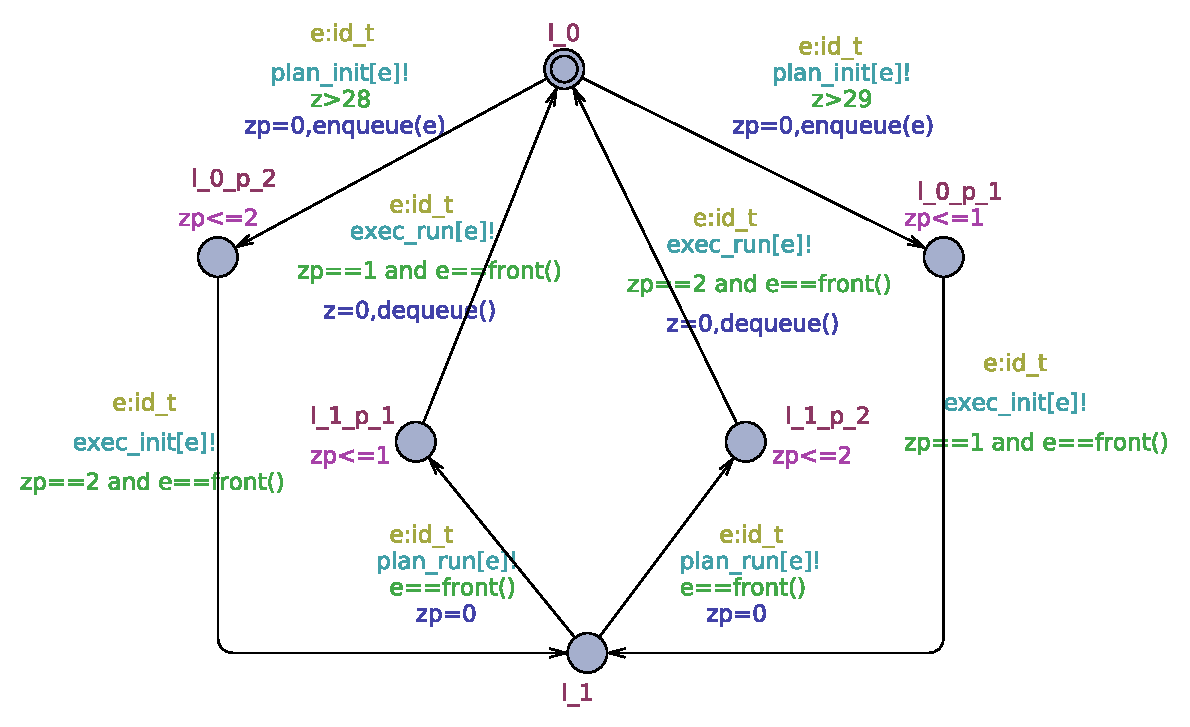
\includegraphics[width=1.15\linewidth]{Figures/c.eps}\\ 
    (a) Controller Component 
  \vspace{4ex}
  \end{minipage}%%
  \begin{minipage}[b]{0.5\linewidth}
  \centering
  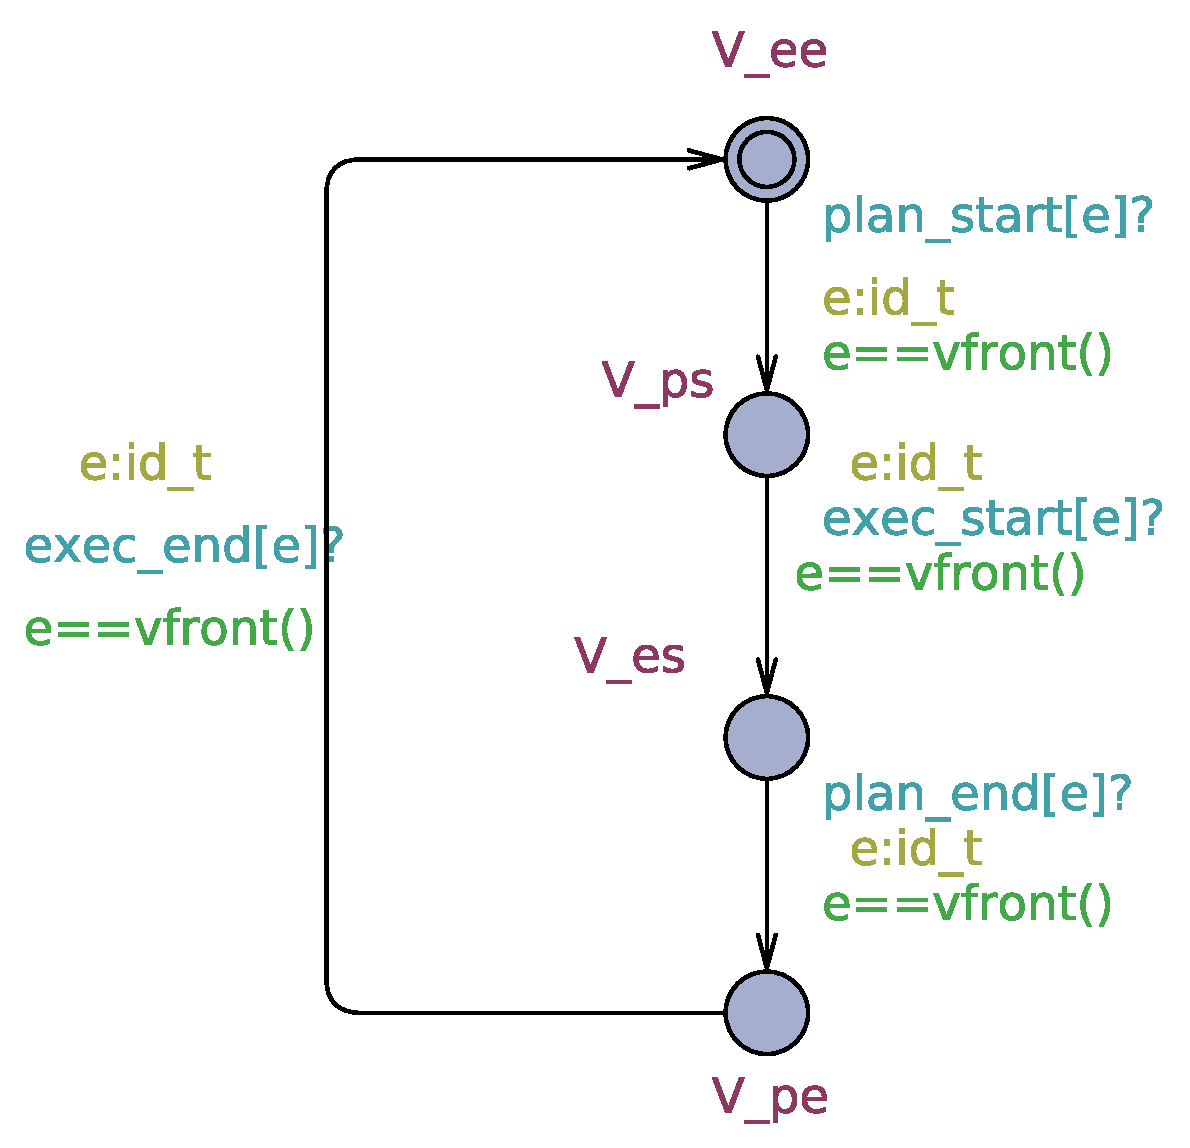
\includegraphics[width=.75\linewidth]{Figures/v.eps}\\ 
    (b) Variable Component 
  \vspace{4ex}
  \end{minipage} 
  \begin{minipage}[b]{\linewidth}
  \centering
  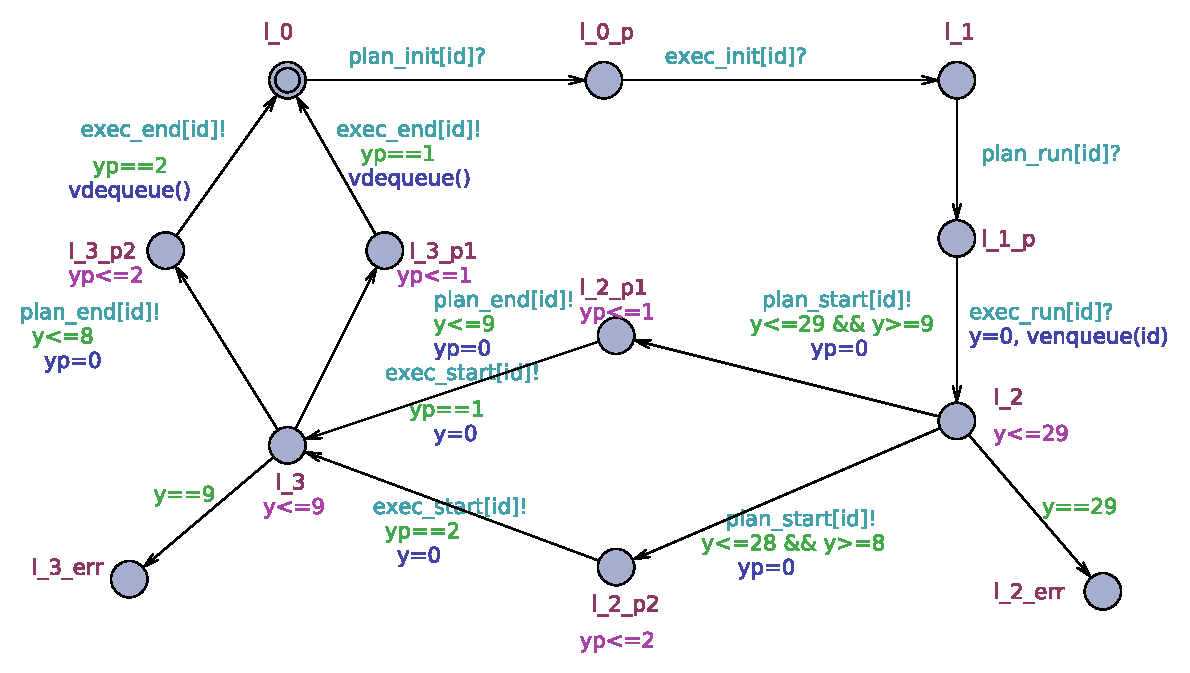
\includegraphics[width=0.75\linewidth]{Figures/t.eps}\\ 
    (c) Task Component 
  \vspace{4ex}
  \end{minipage}%% 
  \caption{Planning Automata for the Task Manager Example}
  \label{fig:uppaal} 
\end{figure}

Once interactions planning encoded, one last thing to do is to add the set of bad states to each
planning automaton (if needed) and find a strategy to avoid those states. 
Figure~\ref{fig:uppaal} depicts the corresponding planning automata for example of 
Figure~\ref{fig:tm} with respect to Definition~\ref{def:plan_aut}. 
Locations suffixed by \emph{p}, correspond to locations following 
planning actions, whereas locations ending with \emph{err} define the bad states, that is,
states with urgent location invariant(s) and no possible execution removing the urgency. 
In this example, for each interaction $\alpha\in\gamma$, we chose $\mathcal{D}(\alpha)=\{1,2\}$.
Notice that for this example, we consider that all actions are controllable actions since
it is a closed system in the sense that there is no interaction with the environment.

We performed the verification on the Task Manager examples with 20 tasks. The winning 
condition being a safety condition: avoid all \emph{\say{err}} locations. This was translated 
into the following property:
\begin{equation}\label{eq:avoid}
  \text{\textsf{control: A[ ] forall (i : int[0,N-1]) not (Task(i).l\_{2\_{err}} or 
  Task(i).l\_{3\_{err}})}}
\end{equation}

The property of interest was successfully verified. Additionally, we were also able to 
synthesize all wining actions of all states using the command line of UPPAAL-Tiga. A sample
of the resulting output is provided below Figures~\ref{fig:sample}.
Notice that the average execution time\footnote{The experiments have been conducted on a HP 
machine with Ubuntu 16.04, an Intel\textsuperscript{\textregistered} 
Core\textsuperscript{\texttrademark}i5-4300U processor of frequency 1.90GHz$\times$4, and
7.7GiB memory.} for verifying Property~\ref{eq:avoid} is $0.1141$ seconds
($0.6534$ seconds when requesting the generation of a strategy).
\begin{figure}[ht]
  \fbox{\begin{minipage}{40em}
    \texttt{State: ( Controller.l\_1\_p\_1 Task(0).l\_0 Task(1).l\_1\_p Task(2).l\_3\_p2 
  Task(3).l\_0 Task(4).l\_0 Task(5).l\_0 Task(6).l\_0 Task(7).l\_0 Task(8).l\_0 Task(9).l\_0 
  Task(10).l\_0 Task(11).l\_0 Task(12).l\_0 Task(13).l\_0 Task(14).l\_0 Task(15).l\_0 
  Task(16).l\_0 Task(17).l\_0 Task(18).l\_0 Task(19).l\_0 Var.V\_pe ) vlist[0]=2 vlist[1]=0
  vlist[2]=0 vlist[3]=0 vlist[4]=0 vlist[5]=0 vlist[6]=0 vlist[7]=0 vlist[8]=0 vlist[9]=0 
  vlist[10]=0 vlist[11]=0 vlist[12]=0 vlist[13]=0 vlist[14]=0 vlist[15]=0 vlist[16]=0 
  vlist[17]=0 vlist[18]=0 vlist[19]=0 vlen=1 Controller.list[0]=1 Controller.list[1]=0 
  Controller.list[2]=0 Controller.list[3]=0 Controller.list[4]=0 Controller.list[5]=0 
  Controller.list[6]=0 Controller.list[7]=0 Controller.list[8]=0 Controller.list[9]=0 
  Controller.list[10]=0 Controller.list[11]=0 Controller.list[12]=0 Controller.list[13]=0 
  Controller.list[14]=0 Controller.list[15]=0 Controller.list[16]=0 Controller.list[17]=0 
  Controller.list[18]=0 Controller.list[19]=0 Controller.len=1\\ 
  When you are in (Controller.zp==1 \&\& Task(2).yp<=2), take transition Controller.l\_1\_p\_1->
  Controller.l\_0 \{ zp == 1 \&\& 1 == front(), exec\_run[1]!, z := 0, dequeue() \}
  Task(1).l\_1\_p->Task(1).l\_2 \{ 1, exec\_run[id]?, y := 0, venqueue(id) \}
  When you are in (Task(2).yp==2 \&\& Controller.zp<=1), take transition Task(2).l\_3\_p2->
  Task(2).l\_0 \{ yp == 2, exec\_end[id]!, vdequeue() \}
  Var.V\_pe->Var.V\_ee \{ 2 == vfront(), exec\_end[2]?, 1 \}}
  \end{minipage}}
  \caption{Sample of the Output Strategy from UPPAAL-Tiga}
  \label{fig:sample}
\end{figure}


\subsection{Discussion}

In this section, we explained how the problem of planning interactions can be formalized into
a real-time controller synthesis approach. However, this approach has some drawbacks.
In order to encode planning of interactions in components as timed automata, this approach
restricts its scope to discretized horizon values which results in having less control
over the planning dates of interactions, and leads in case of a high number of discretized 
values, to an explosion in the number of planning transitions. Unfortunately, we do not 
have an immediate solution for this problem. In fact, it is user dependent since one user may 
just want to have a ASAP execution for a given interaction, for instance because the components
involved in this interaction are often requested, and in that case the practice will be to 
always plan with $\hmin$. In other cases, the user may want to plan an interaction with 
flexible amount time.
Additionally, this approach considers only a class of systems where interactions have timing 
constraints on up to one of their participating components action. Otherwise, the planning 
should be encoded on the composition, which represents a tedious work because of the state 
space explosion problem. Nevertheless, this approach differs form the usual scheduler 
synthesis approach since it is not performed on the regular semantics of timed automata. 
Particularly, here we are interested in avoiding bad states of the planning semantics 
(states that verify the expression of Theorem~\ref{thm:dla}). Consequently, unless finding an 
automatic general method for generating such complex expression in the query language accepted 
by such tools, and without ignoring that finding a strategy avoiding those states 
may be hard in term of computational complexity, our real-time controller synthesis approach 
seems more straightforward and much simpler but it comes with some feasibility restriction.














%\chapter{Clock Drift}\label{chap:6}
\minitoc

In the previous section, we introduced a timed automata model that 
describes a high level representation of systems execution. 
However, this type of model assumes that components clocks are perfectly synchronous which is 
hardly the case in practice.
Effectively, clocks are able to measure time up to a certain precision and will be likely
to drift since they are implemented based on oscillators that are not perfect: the oscillator 
frequency is not constant, it changes depending on environmental conditions such as 
temperature, humidity and aging.
Figure~\ref{fig:drift_exp} illustrates an example of two clocks $x$ and $y$ having different rate
with respect to an implicit perfect reference time. Figure (a) shows the case
where clock $x$ evolves steadily faster than clock $y$. Whereas, in Figure (b) 
clock $y$ is initially faster than clock $x$, then the trend is inverted after some time.

\begin{figure}[ht] 
\begin{minipage}[b]{0.5\linewidth}
\centering
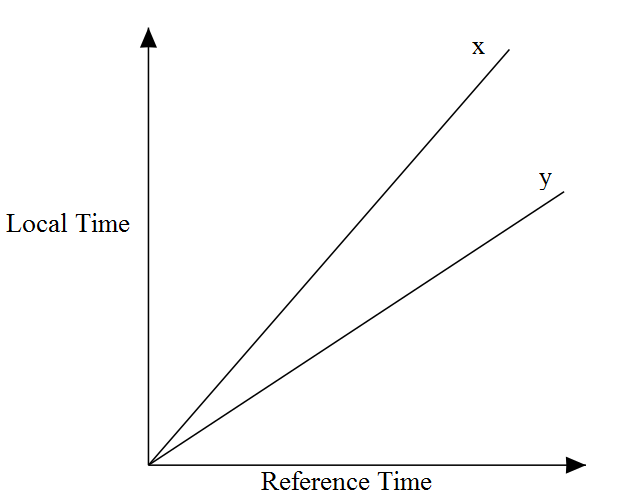
\includegraphics[scale=.55]{Figures/drift1}\\ 
  \vspace*{5mm} \small{(a)} 
\vspace{4ex}
\end{minipage}%%
\begin{minipage}[b]{0.5\linewidth}
\centering
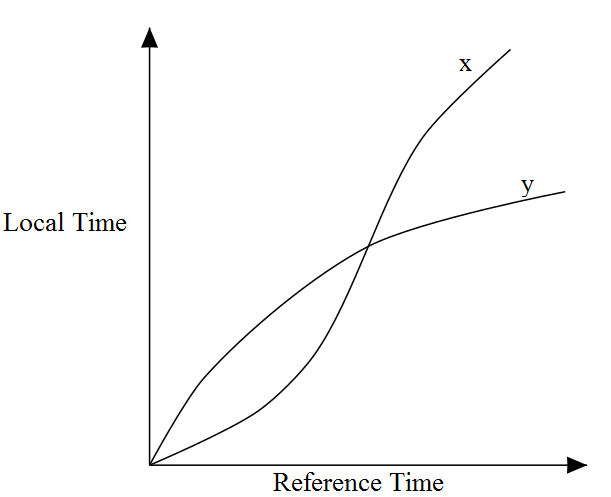
\includegraphics[scale=.55]{Figures/drift2}\\ 
  \vspace*{5mm} \small{(b)}
\vspace{4ex}
\end{minipage} 
\caption{Example of Clocks with Different Rates}
\label{fig:drift_exp}
\end{figure}

In this chapter, we present a distributed timed automata model where clocks advance at 
different rates and we study the resulting effect on the system behavior.

\section{Distributed Timed Systems with Independent Clock Rates}

\subsection{Expressing Clock Constraints Using Local Clock}

When building distributed real-time systems, a common practice is to use 
local clocks as time references as explained in Chapter~\ref{chap:3}.
These clocks measure the absolute time elapsed since the system startup and are never reset. 
This approach reduces the effort of keeping track of the actual time progress in components
and enable to have a common time scale. 

The idea consists in mapping each clock of a component to a (unique) local clock.
Thus, the value of component clocks are obtained by simply shifting their corespondent local 
clock by a constant amount of time as soon as the clocks are not reset.
Effectively, for each clock $x$ of a component, we introduce a real variable $\rho_x$ that 
stores the absolute time of its last reset (with respect to its local clock), that is, if $x$ 
is mapped to a local clock $g$, then each time $x$ is reset, $\rho_x$ is update to the current 
value of g.
Notice that the value of $x$ can be found by the equality $x=g-\rho_x$.
As a result, any timing constraints $c$ of a component $B_i$ can be expressed using a 
local clock $g$ as follows:
\begin{equation}
  \label{eq:glob}
  c = \bigwedge_{x_i\in\X_i} l\triangleleft x_i\triangleright u
    =\bigwedge_{x_i\in\X_i} l+\rho_{x_i}\triangleleft g\triangleright u+\rho_{x_i}
\end{equation}

where $\triangleleft\in\{<,\le\}$ and $\triangleright\in\{>,\ge\}$.
Notice any timing constraints of Definition~\ref{eq:cc} can be written on the form of 
inequalities. 


\subsection{Distributed Timed System}

Let $S=(\Loc,\loc_0,\X,\D,\gamma,\E_{\gamma},\{f_e\}_{e\in\gamma},\I)$ be a timed system of $n$ 
components synchronizing through the interaction set $\gamma$. 
For an interaction $\alpha$, we denote by $\clock{\alpha}$ the set of clocks appearing in its
timing constraints, that is, $\clock{\alpha}=\{x\in\X|\forall (\loc,\alpha,g,r,\loc')\in
\E_{\gamma}, x \ \circlled{$\in$} \ g \}$, with \circlled{$\in$} denoting the presence of
$x$ in the guard $g$.

Given an interaction partition $\{\gamma_k\}_{k=1}^m$, we put $\clock{\gamma_k}$ to denote
the set of clocks appearing in the timing constraints of interactions of $\gamma_k$, that is,
$\clock{\gamma_k}=\{\cup_{\alpha\in\gamma_k}\clock{\alpha}\}$.
We formalize the independent evolution of clocks by defining an \emph{ownership map} that assigns
a set of clocks to a unique local clock based on interaction partitioning . 
Particularly, we assign to each class of interaction a unique local clock. 
We require additionally that clock of each components is mapped only to a unique local clock.
This avoid timing inconsistency and ensure that each clock of a component is evaluated using 
a unique local 
clock. This constraints immediately the interaction partitioning as follows:
\begin{equation}\label{eq:tcf}
  \bigwedge_{\substack{i,j\in\{0,\cdots,m\}\\i\neq j}}\clock{\gamma_i}\cap\clock{\gamma_j}=
  \emptyset
\end{equation}

\begin{definition}[Distributed Timed System]\label{def:drft}
Given a timed system $S=(\Loc,\loc_0,\X,\D,\gamma,\E,$\\$\{f_e\}_{e\in\gamma},\I)$
and an interaction partitioning satisfying the constraint~\ref{eq:tcf}. 
We define the corresponding distributed timed system with independent local clock rates
as the tuple  
  $S^{dt}=(\Loc,\loc_0,\X^{dt},\D^{dt},\gamma,\E^{dt},\{f_e^{dt}\}_{e\in\gamma},\I^{dt},\pi)$ 
such that:
\begin{itemize}
  \item $\X^{dt}$ is the set of local clocks (a unique clock per class of interaction) 
  \item $\pi:\X\lto\X^{dt}$ is a many to one mapping between clocks $\X$ of $S$ and local clocks 
    $\X^{dt}$
  \item $\D^{dt}=\D\cup\{\cup_{x\in\X}\rho_x|\rho_x\in\realpoz\}$ is the set of data with 
    $\rho_x$ being real valued variables storing absolute reset times
  \item $\E^{dt}$ is such that for every $(\loc,\alpha,g,r,\loc')\in\E$, $\alpha\in\gamma$, we 
    have the corresponding transition $(\loc,\alpha,g^{dt},\emptyset,\loc')\in\E^{dt}$ where:
  \begin{itemize}
    \item $g^{dt}$ is the guard $g$ expressed using the local clock $x^{dt}\in\X^{dt}$ where
      $\forall x_i,x_j\in\clock{\alpha},i\neq j,\pi(x_i)=\pi(x_j)=x^{dt}$
    \item $f_e^{dt}=f_e\cup\{\rho_x:=x^{dt}|\forall x\in r\}$ is the transfer function updating 
      reset variables in addition to data variables of $\D$
  \end{itemize}
  \item $\I^{dt}$ is the set of location invariants expressed using local clocks 
\end{itemize}
\end{definition}

Notice that clocks appearing in location invariants appear necessarily in at least an 
interaction since we assume timed system with well formed guard.

\begin{property}[Semantics]
  The semantics of a distributed timed system $S^{dt}=(\Loc,\loc_0,\X^{dt},\D^{dt},$\\$\gamma,
  \E^{dt},\{f_e^{dt}\}_{e\in\gamma},\I^{dt},\pi)$ is defined by the timed transition system 
  $\ttsb{dt}=(\Q^{dt},q_0^{dt},\gamma,\lto_{\gamma})$ where:
  \begin{itemize}
    \item $\Q^{dt}=\Loc\times\V(\X_{dt}\cup\tcal{D}_{dt})\times\Delta$ where $\Loc$ is 
      the set of global locations, $\V(\X_{dt}\cup\tcal{D}_{dt})$ is the set of clock and 
      data valuations, and $\Delta=\real$ is the set offsets of local clocks in 
      $\X_{dt}$ with respect to an implicit (perfect) reference clock 
    \item $q_0^{dt}=(\loc_0,0,0)$ is the initial state.
    \item $\lto_{\gamma}\subseteq\Q^{dt}\times(\gamma\cup\realpos)\times\Q^{dt}$ is the set of 
      labeled transitions defined by the rules:
    \begin{itemize}
      \item $(\loc,\val,\delta)\transit{\alpha}_{\gamma}(\loc',\val[r],\delta)$ for 
        $\alpha\in\gamma$, if
      $(\loc,\alpha,g,r,\loc')\in\E^{dt}\wedge \val\models g$
    \item $(\loc,\val,\delta)\transit{d}_{\gamma}(\loc,\val',\delta')$ for $d\in\realpos$, 
      such that $\val'=\val+d-\delta+\delta'\wedge \val'\models\I^{dt}(\loc)\wedge\val'\ge\val$
    \end{itemize}
  \end{itemize}
\end{property}

The above semantics models drifting clocks by introducing an offset variable $\delta$ that 
stores for each clock in $x^{dt}$ its actual drift value with respect to an implicit 
reference time. The common practice when clocks are subject to drift is to
\emph{regularly resynchronize} the clocks using different methods, such as bit-stuffing 
or any other clock synchronization scheme.
Consequently, we consider a more realistic model where clocks can drift up
to a certain value $\epsilon$ with respect to a reference clock. This value is generally 
computed based on three parameters: \emph{(i)} the post-synchronization gap, \emph{(ii)} 
the longest gap between synchronizations, and \emph{(iii)} the clock precision parameter 
usually given by the constructor.
This induces that $\delta\in[-\epsilon,\epsilon]^{|\X^{dt}|}$.


\subsection{Properties}

\begin{property}\label{pr:rd}
  $\forall x,y\in\X^{dt},x\neq y,\delta=(\cdots,\delta_x,\cdots,\delta_y,\cdots)$
  where $|\delta|=|\X^{dt}|$, we have $\delta_x-\delta_y\in[-2\epsilon,2\epsilon]$
\end{property}

Property~\ref{pr:rd} states that the relative drift between local partitions 
clock is bounded by $2\epsilon$. This results from the fact that all local
clocks are kept within $\epsilon$ of a reference clock.

In order to attest the correctness of the distributed semantics, we compare
its corresponding time transition system ($\ttsb{dt}$) and the timed transition system 
of the standard semantics ($\ttsb{g}$).

Let $R$ be the relation:
\begin{align*}
  R=\{(q^{dt},q)\in\Q_{dt}\times\Q|q^{dt}=(\loc^{dt},\val^{dt},\delta), q=(\loc,\val) \\
  \text{ such that: }  
  \begin{cases}
  \loc^{dt}=\loc,\\
  \forall x\in\X,\val(x)=\valdt(\pi(x))-\rho_x-\delta_x  
\end{cases}
\end{align*}

The relation $R$ relates states of the distributed semantics with
states of the standard semantics having the same location configuration,
and whose clock valuations expressed on local clocks are $\delta\in[-\epsilon,\epsilon]$ close. 
We call such states $\epsilon-$similar.

\begin{lemma}\label{lem:equiv}
  For $\epsilon=0$, we have $\ttsb{dt}\sim_{R}\ttsb{g}$ 
\end{lemma}

Lemma~\ref{lem:equiv} describes the fact that a given system and its corresponding 
distributed model are bisimilar when $\Delta=0$, that is, when clocks advance at the same 
rate (perfect clocks). 

\begin{property}\label{pr:enabled1}
  Let $(\qdt,q)\in \RS$ such that $\qdt$ satisfies $\enabled{\alpha}$, then
  $q$ satisfies \\$\enabledbackwardb{\alpha}{0}{\epsilon}\vee\enabled{\alpha}
  \vee\enabledforwardb{\alpha}{0}{\epsilon}$.
\end{property}

Property~\ref{pr:enabled1} expresses that for states $(\qdt,q)\in\RS$ if it exists
an interaction enabled at $\qdt$ then this interaction is either enabled at $q$, 
will be enabled after a time progress of $\epsilon$ or is up to $\epsilon$ after 
the deadline of $\alpha$. This property flows directly from the $\epsilon-$similarity
of states $(\qdt,q)\in\RS$, the form of interactions timing constraints 
(conjunction of intervals)
and the fact that clocks involved in the same interaction advance at the same rate. 
It points out that any execution from
state $\qdt$ might not be always possible from state $q$ or any of its time successor.

\begin{lemma}\label{lm:enabled1}
  Let $(\qdt,q)\in\RS$ such that $\qdt$ satisfies $\enabled{\alpha}\wedge
  \enabledbackwardb{\alpha}{\epsilon}{\epsilon}$, then
  $q$ satisfies $\enabledbackwardb{\alpha}{0}{\epsilon}$.
\end{lemma}
Lemma~\ref{lm:enabled1} can be deduced straightforwardly from property~\ref{pr:enabled1}.
It expresses that for states $(\qdt,q)\in\RS$, if it exists an interaction $\alpha\in\gamma$
such that $\alpha$ is enabled at $\qdt$ and that clock valuations are up to $\epsilon$ 
before the deadline of this interaction then, $\alpha$ can be executed from $q$ or any of its 
$\epsilon-$time successors (by doing a time progress up to $\epsilon$).

The usual notion of simulation as defined in~\ref{def:sim} is too precises. 
It requires that each trace in one system
can be matched~\emph{exactly} by a trace in the other system, that is, 
two states can be distinguished even for an infinitesimally
small mismatch between timings ($\epsilon\neq0$). 
Thus, we rely on the following quantitative variant of simulation~\cite{drift:esim}. 

\begin{definition}[$\epsilon-$simulation]\label{def:esim}
  Given two TTS, $\TTSc{1}$ and $\TTSc{2}$, a relation $R\subseteq\Q_1\times\Q_2$ is a:
  \begin{itemize}
    \item Strong timed $\epsilon-$simulation, if for any $(q_1,q_2)\in R$, $\sigma\in\sum$, 
      $d,\epsilon\in\realpoz$
    \begin{itemize}
      \item $q_1\transit{\sigma}\q_1'$ implies $q_2\transit{\sigma}q_2'$ for some $q_2'\in\Q_2$ 
        with $(q_1',q_2')\in R$
      \item $q_1\transit{d}\q_1'$ implies $q_2\transit{d'}q_2'$ for some $q_2'\in\Q_2$ and 
        $d'\in\realpoz$ with $|d'-d|\le\epsilon$ and $(q_1',q_2')\in R$
    \end{itemize}
    \item Timed action $\epsilon-$simulation, if for any $(q_1,q_2)\in R$, $\sigma\in\sum$, 
      $d,\epsilon\in\realpoz$
    \begin{itemize}
      \item $q_1\transit{d,\sigma}\q_1'$ implies $q_2\transit{d',\sigma}q_2'$ for some $q_2'
        \in\Q_2$ and $d'\in\realpoz$ with $|d'-d|\le\epsilon$ and $(q_1',q_2')\in R$
    \end{itemize}
  \end{itemize}
  If there exists a strong timed (resp. timed action) $\epsilon-$simulation
  between $\ttsb{1}$ and $\ttsb{2}$ w.r.t $R$, then we write
  $\ttsb{1}\sqsubseteq^{\epsilon}_{R}\ttsb{2}$ (resp. $\tts{1}\sqsubseteq^{\epsilon*}_{R}
  \ttsb{2})$
\end{definition}


This approach characterizes
the degree of closeness between timed systems: it generalizes the (boolean) 
notions of timed simulation
(yes or no) to metrics over timed system. Formally, for a positive real number
$\epsilon$, a state $q_1$ is 
told $\epsilon-$similar to another state $q_2$ if there is a time-abstract simulation 
that can relates both states in
the sense that the difference between the delays of time-step transitions is at most $\epsilon$.

Although this definition of simulation is less 
restrictive, Property~\ref{pr:enabled1} gives the intuition that for some states
$(\qdt,q)\in\RS$ there may be interactions that can be executed from $\qdt$ but not from
$q$, which make the $\epsilon-$simulation impossible.

\section{Robust Distributed Semantics}
As explained in previous sections, the distributed semantics may 
exhibit new behavior with respect to the standard semantics.  
In this section, we identify the problematical states of the 
distributed semantics and provide sufficient conditions
that will guarantee timed action $\epsilon-$simulation. 

\begin{definition}[Potentially Bad States]\label{def:pbss}
  We denote by $\Upsilon$ the set of potentially bad states of the 
  distributed semantics characterized as follows:
  \[\Upsilon=\{q=(\loc,\val)|\exists\alpha\in\gamma,\val\models g_{\alpha}\wedge
  \val+\epsilon\not\models g_{\alpha} \} \]
\end{definition}

The intuition behind this characterization results form Property~\ref{pr:enabled1}.
These states may yield possible execution of interactions in the distributed semantics that
are not possible in the related states of the standard semantics (states that are 
$\epsilon-$similar). 

\begin{proposition}\label{prop:esim}
  Let $\ttsb{dt}$ be the timed transition system of the distributed semantics. 
  We have: 
  \[\Upsilon\cap\reach^*(\ttsb{dt})=\emptyset\implies\ttsb{dt}\sqsubseteq^{\epsilon*}_{\RS}
  \ttsb{g}\]
  where $\reach^*(\ttsb{dt})$ is the projection of states of the distributed semantics 
  on state variables of the standard semantics, that is, by considering only locations, clocks,
  and data variables.
\end{proposition}

\begin{proof}[Proof of Proposition~\ref{prop:esim}]
  
  In order to prove proposition~\ref{prop:esim}, we need to show that if for any 
  $(\qdt,q)\in\RS$, $\sigma\in\gamma$ and $d\in\realpoz$:
      \begin{displaymath}
        \qdt\transit{d,\sigma}\qdtb \implies \exists q'\in\Q^g, q\transit{d',\sigma}q',
        \text{ with } 
        d'\in\realpoz, \ |d'-d|\le\epsilon \text{ and } (\qdtb,q')\in\RS
      \end{displaymath}
       
      Let $(\qdt,q)\in\RS$ such that $\Upsilon\cap\reach^*(\ttsb{dt})=\emptyset$ and 
      $\exists\sigma\in\gamma,\exists d\in\realpoz,$ 
  $\qdt\transit{d,\sigma}\qdtb$. We distinguish two cases:
  \paragraph{\textbf{Case 1: $d > 0$}\\}
  We have $\qdt \transit{d,\sigma}\qdtb$. This means:
    \[
    \begin{cases}{}
      \valdtb=(\valdt+d-\delta+\delta')[r^{dt},f_{\sigma}] \\  
      \valdt +d-\delta+\delta'\models\I^{dt}(\loc)\wedge g_{\sigma}^{dt} \\ 
      \valdt +d-\delta+\delta'+\epsilon\models\I^{dt}(\loc)\wedge g_{\sigma}^{dt}& 
      \qdt\notin\Upsilon 
    \end{cases}\]
  where $[r^{dt},f_{\sigma}]$ means after applying reset and transfer function.
  When expressed on original clocks the above becomes:
    \[\begin{cases}{}
      \valdtb=(\val+\rho+d+\delta')[r^{dt},f_{\sigma}]\\ 
      \val+d+\delta'\models\I(\loc)\wedge g_{\sigma} \\ 
      \val+d+\delta'+\epsilon\models\I(\loc)\wedge g_{\sigma} 
    \end{cases}\]
  We also have $\delta'\in[-\epsilon,\epsilon]$. Consequently we have: 
  
  \begin{enumerate}
    \item $\delta'\in[0,\epsilon]$, then:\\
      \[\begin{cases}{}
        \valdtb=\val+d+\delta'+(\rho)[r^{dt},f_{\sigma}]\\ 
      \val+d+\epsilon\models\I(\loc)\wedge g_{\sigma} \label{1} 
    \end{cases}\]
    By putting $d'=d$, and  since $r^{dt}=\emptyset$ (Definition~\ref{def:drft}) and 
      $f_{\sigma}$ applies only on $\rho$ we obtain: 
      \[\begin{cases}
        \valdtb=\val+d'+\delta'+(\rho)[r^{dt}] \\ 
      \val+d'+\epsilon\models\I(\loc)\wedge g_{\sigma} \label{1} 
      \end{cases}\]%%%%%
      Consequently, we can conclude that $q\transit{d',\sigma}q'$ such $(\qdtb,q')\in\RS$
    \item $\delta'\in[-\epsilon,0]$, then:\\
      \[\begin{cases}{}
        \valdtb=\val+d+\delta'+(\rho)[r^{dt},f_{\sigma}]\\ 
      \val+d-\epsilon+\epsilon\models\I(\loc)\wedge g_{\sigma} \label{1} 
    \end{cases}\]
    By putting $d'=d$, and  since $r^{dt}=\emptyset$ (Definition~\ref{def:drft}) and 
      $f_{\sigma}$ applies only on $\rho$ we obtain: 
      \[\begin{cases}
        \valdtb=\val+d'+\delta'-\epsilon+(\rho)[r^{dt}] \\ 
      \val+d'\models\I(\loc)\wedge g_{\sigma} \label{1} 
      \end{cases}\]%%%%%
      Consequently, we can conclude that $q\transit{d',\sigma}q'$ such $(\qdtb,q')\in\RS$
  \end{enumerate}
  
  \paragraph{\textbf{Case 2: $d = 0$}\\}
   Since $\Upsilon\cap\reach^*(\ttsb{dt})=\emptyset$, using the same methodology of case 1, 
   we can conclude that $\exists q'\in\Q^g, q\transit{d',\sigma}q',\text{ with } 
        d'\in\realpoz, \ |d'-d|\le\epsilon \text{ and } (\qdtb,q')\in\RS$.
\end{proof}

Proposition~\ref{prop:esim} highlights an interesting property on the reachable states of the 
distributed semantics. It states that if all the reachable states of the 
distributed semantics are not potential bad states, i.e, $\Upsilon\cap\reach^*(\ttsb{dt})=
\emptyset $, then there exists a timed action $\epsilon-$simulation between the timed transition 
systems of the standard semantics and the distributed semantics.

Consequently, the idea is to restrict the distributed semantics in order to
avoid such states. 
This can be achieved by shrinking the upper bound of every transition timing constraints, if it 
exists, by $\epsilon$.   
Let $\ttsb{\dte}$ be the timed transition system after shrinking every existing upper bound timing
constraints by an amount of $\epsilon$. Then, we have the following lemma:
\begin{lemma}
  $\ttsb{\dte}\subseteq\ttsb{dt}$
\end{lemma}
The above lemma derives straightforwardly from the fact that shrinking does not introduce new
behavior. Conversely, it just restrains the set of states from which interactions can be 
executed.

\begin{lemma}\label{lem:shrink}
  $\Upsilon\cap\reach^*(\ttsb{\dte})=\emptyset$.
\end{lemma}
The above lemma is a direct consequence of the shrinking operation.   
In fact, since clocks of the distributed semantics an those of the standard semantics can have
at most $\epsilon$ difference in values, by shrinking upper bound timing constraints we avoid
all possible execution of interactions for clock values that are $\epsilon$ before its due date.
Consequently, this ensures that $\Upsilon\cap\reach*(\ttsb{\dte})=\emptyset$ and allows for any 
related state of the standard semantics to execute the same interaction
directly or after doing a timed step. 
%This can be effectively achieved by restricting the progress of time based to 
%$\epsilon$ before the due date of interactions.
%Preventing the progress of time $\epsilon$ time units
%before any interaction deadline will prevent any execution not possible 
%in the corresponding state of the standard semantics.
%Formally, this restriction can be written as follows:
%\begin{equation}\label{eq:res}
% (\loc,\val,\delta)\transit{d}_{\gamma}(\loc,\val',\delta') \text{ for } d\in\realpos, 
%      \text{ such that }\val'=\val+d-\delta+\delta'\wedge \val'\models\I(\loc)\wedge
%      (\loc,\val',\delta')\notin\Upsilon
%\end{equation}

%The above restriction of time progress helps to avoid reaching the potential bad states
%characterized by Definition~\ref{def:pbss}. However, this restriction does not guarantee 
%the non-reachability of such states. In fact, interaction executions may as well lead 
%to state of $\Upsilon$. Consequently, to prove that any reachable state of the distributed
%semantics is not a potentially bad state, we need to ensure that any \emph{arrival state},
%that is, state reachable immediately after the execution of an interaction is not a potentially
%bad state.
The following lemma is a direct consequence of Proposition~\ref{prop:esim} and Lemma~\ref{lem:shrink}.
\begin{lemma}
  $\ttsb{\dte}\sqsubseteq^{\epsilon*}_{\RS}\ttsb{g}$
\end{lemma}

\begin{definition}[Robustness]\label{def:rob}
  For a given timed system S, we say that S is robust to clock drifts iff $\reach(\ttsb{\dte})$ 
  is deadlock free.
\end{definition}

Restricting the distributed semantics through shrinking allows to avoid the reachability of some states 
(the potential bad states). This enforces the timed action $\epsilon-$simulation between states
of the standard semantics and those of the restricted distributed semantics.
However, since shrinking reduces the set of reachable states, the timed action $\epsilon-$simulation
alone is not enough. We must also ensure that shrinking does not introduce any deadlocks. 
The two aforementioned point together form our definition of robustness.

\section{Discussion}

In this chapter, we revisited the robustness concept usually used to check whether a given
system still satisfies the specification (a set of properties) when subject to different
perturbations such as clock drift. We first modeled the behavior of a timed system with 
independent clock rates and subject to a resynchronization scheme. Thereafter, we used
a variant of simulation that relates states with a timing difference up to a certain $\epsilon$,
and provide a characterization of potential bad states that may invalidate this variant of 
simulation. Then, we suggested a strategy based on shrinking upper bound timing constraints
in order to avoid such states which allows to attest the timed action $\epsilon-$simulation.

Sankur et al.~\cite{ocan} studied the robustness problem in timed automata against guards
shrinking. They provided a method for deciding whether shrinking all timing constraints (guards)
of a timed automaton, by possibly different amounts, results in a timed automaton that 
preserves some time-abstract behaviors, and is not blocking. The latter represents their
robustness notion.
It was proven that if the automaton is shrinkable, then several properties established on the 
initial automaton are preserved in the implementation (when clocks are not perfect). 
Otherwise, then the conclusion is that the model is vulnerable to the slightest variations in the 
measure of time and should thus be considered as non-robust, and the design should be reviewed.
From a theoretical aspect, the proposed analysis was formulated as a parameter synthesis
problem. \texttt{Shrinktech}~\cite{ocan2} is a tool that implements the simulation-shrinkability 
algorithm presented in~\cite{ocan}. It is compatible with the Kronos~\cite{kronos} model checker,
that can minimize the region graph of a timed automaton~\cite{tl} needed by the tool.
The tool has been used to attest the shrinkability of several case studies, such as 
the Philips Audio Retransmission protocol, Fischer's Mutual
Exclusion protocol (up to 4 agents), and some other asynchronous circuit models.
These experiments showed that the tool is capable of treating shrinkability of timed automata 
with thousands of edges (w.r.t graphs with more than sixty thousand transitions).
The bottleneck of the tool was also identified as being the size of the full bisimilarity graph,
which is often costly to compute, and that may require long processing time for shrinkability analysis. 
Moreover, the non-shrinkability of most models was mainly due equality constraints, or to the fact
that some models was designed at a high level of abstraction where imprecisions were
not taken into account.





%\chapter{Implementation and Experimentation}
\label{chap:7}
\minitoc
\section{The BIP Framework}

BIP~\cite{intro:bip} is a highly expressive model-based and component-based framework for 
building embedded applications. It is based on three main layers: Behavior, interactions, and
priorities as shown in Figure~\ref{fig:bip_layers}:
\begin{figure}[ht]
\centering

\begin{tikzpicture}[remember picture]

\node[rectangle,draw=blue!50,fill=blue!20](b){B};
\node[rectangle,draw=blue!50,fill=blue!20,right=2mm of b,minimum width=6mm,minimum height=2mm](e)
{E};
\node[rectangle,draw=blue!50,fill=blue!20,right=2mm of e,minimum width=6mm,minimum height=2mm](h)
{H};
\node[rectangle,draw=blue!50,fill=blue!20,right=2mm of h,minimum width=6mm,minimum height=2mm](a)
{A};
\node[rectangle,draw=blue!50,fill=blue!20,right=2mm of a,minimum width=6mm,minimum height=2mm](v)
{V};
\node[rectangle,draw=blue!50,fill=blue!20,right=2mm of v,minimum width=6mm,minimum height=2mm](i)
{I};
\node[rectangle,draw=blue!50,fill=blue!20,right=2mm of i,minimum width=6mm,minimum height=2mm](o)
{O};
\node[rectangle,draw=blue!50,fill=blue!20,right=2mm of o,minimum width=6mm,minimum height=2mm](r)
{R};
\node[rectangle,draw=red!50,fill=red!20,above=2mm of a,inner xsep=21.15mm,xshift=4.35mm](inter)
{Interactions};
\node[rectangle,draw=yellow!50,fill=yellow!20,above=2mm of inter,inner xsep=23.35mm](inter)
{Priorities};

\begin{scope}[on background layer]
\node[fit=(inter)(b)(r),fill=gray!20,draw=gray!50]{};
\end{scope}

\end{tikzpicture}
\caption{BIP Layers}
\label{fig:bip_layers}
\end{figure}

\begin{itemize}
  \item Behavior: This layer describes the behavior of each component of a system as a timed
    transition system. Atomic components are defined as timed automata with well defined 
    interface (ports).
  \item Interactions: The interaction layer specifies how components interact together and
    coordinate their action using n-ary synchronizations. It restricts thus the global behavior 
    of components together using these synchronizations.
  \item Priorities: Priorities are used to favor the execution of a subset of enabled 
    interactions called \emph{maximal} interactions. They can be used to resolve conflicts or to
    express particular scheduling policies.
\end{itemize}

The Real-Time BIP language~\cite{rtbip} extends the BIP language through clocks used to express
timing constraints on transitions and locations (location invariants). 
It also supports urgency types on transitions~\cite{urg} that provide additional means to 
constrain the progress of time in a given system.
In this thesis, we do not consider priorities or urgency types. However, given a timed system
$S$ that includes priority rules on interactions and/or urgency types on transitions, 
then its underlying timed transition system $\tts_S$ is included in the timed
transition system representing its abstraction $S^*$ from the latter, that is,
$\tts_S\subseteq\tts_{S^*}$. This means that all the results of this thesis, if they apply
on $S^*$, then they apply on $S$.

The BIP language defines systems as a composition of components using a set of syntactic
constructs that specify components behavior and interface as well as the ongoing 
synchronizations (interactions) and priorities. They consist of the following:

\begin{itemize}
  \item Atomic component: Atoms represent the simplest entity of a system. An atomic component
    may include a set of ports, data and clocks. Its behavior is described using an 
    automaton or a Petri net whose transitions are labeled by ports with guards possibly on data 
    and/or clocks. Ports and data can be exported, and thus become accessible at a higher
    hierarchy level (compound). They define the interface of a component.
    Additionally, atomic components support the usage of external C/C++ functions on
    transition guards and may as well trigger the execution of such functions on the
    execution of a transition. 
  \item Connector: Connectors are stateless entities that characterize the possible interactions
    between a set of components via their interface ports.
  \item Priority: Priorities are used to restrict the possible set of enabled interactions.
  \item Compound: A compound is a composite component that consists of a set of atomic 
    components, the connectors specifying their interactions and a set of priority rules. It
    may as well export ports and data.
  \item Package: A BIP package is a compilation unit contained in a single .bip file. It may
    contain data, external data types, external functions, external operators, port types,
    atom types, connector types and compound types. It also may use other BIP packages.
\end{itemize}
\begin{example}\label{exp:bip}
Figure~\ref{lst:bip} illustrates the syntax of BIP and presents different elements of the BIP 
  language. The package \emph{ControllerWorker} includes the definition of the
  port type \emph{Port}, the connector type \emph{Link} for interactions involving two 
  ports of type \emph{Port}, atomic components \emph{Controller} and \emph{Worker}.
  The atomic component \emph{Controller} consists of a clock $x$, an internal port \emph{init}
  and two exported port, $a$ and $c$, defining its interface. The statement 
  \texttt{place lc0, lc1, lc2} defines the places (locations) of the timed automaton describing its behavior,
  where \texttt{lc0} is the initial place. Lines 19 to 22 represent the declaration of 
  a transition. It consists of the following elements:
  \begin{enumerate}
    \item The port labeling the transition: \texttt{\textbf{on} init}
    \item The source and destination places: \texttt{\textbf{from} lc0 \textbf{to} lc1}
    \item A possible empty list of guards over data and clocks: \texttt{\textbf{when} 
      $x\ge 8$ second}
    \item A possible empty list of clocks to reset: \texttt{\textbf{reset} x}
    \item A possible empty transfer function for updating data variable or triggering the 
      execution of external C code: \texttt{\textbf{do}\{\}}
  \end{enumerate} 

As explained earlier, components are composed using connectors. The Compound Type \emph{System}
defines a system composed of two Workers and one Controller. It also defines the interactions 
between the \emph{controller} component and each \emph{Worker} component ($worker_1$ and 
$worker_2$) through connectors $ab1$, $cd1$, $ab2$, and $cd2$.
\end{example}
\begin{figure}[H]
\begin{lstlisting}[basicstyle=\ttfamily,
escapeinside={||},
mathescape=true,
numbers=left,
backgroundcolor=\color{gray!20}]
|\textbf{package}| ControllerWorker

  |\textbf{port type}| Port()
  
  |\textbf{connector type}| Link (Port p1, Port p2)
    |\textbf{define}| p1 p2
  |\textbf{end}|

|\textbf{atom type}| Worker()
  |\textbf{clock}| y 
  
  |\textbf{export port}|  Port d()
  |\textbf{export port}|  Port b()
  
  |\textbf{place}| l1, l2
 
 |\textbf{initial}| to l1

  |\textbf{on}| b
    |\textbf{from}| l1 |\textbf{to}| l2
    |\textbf{when}| ( y>= 5 )
    |\textbf{do}| {}

  |\textbf{on}| d
    |\textbf{from}| l2 |\textbf{to}| l1
    |\textbf{reset}| y
    |\textbf{do}| {}
|\textbf{end}|
|\textbf{atom type}| Controller()
  |\textbf{clock}| x 
  |\textbf{export port}|  Port a()
  |\textbf{export port}|  Port c()
  |\textbf{port}| Port init()


\end{lstlisting}
\end{figure}


\begin{figure}[H]
\begin{lstlisting}[basicstyle=\ttfamily,
escapeinside={||},
mathescape=true,
numbers=left,
backgroundcolor=\color{gray!20},
firstnumber=37]
  |\textbf{place}| lc0, lc1, lc2
  
  |\textbf{initial to}| lc0
    |\textbf{do}| {}
  
  |\textbf{on}| init
    |\textbf{from}| lc0 |\textbf{to}| lc1
    |\textbf{when}| (x >= 8 second) 
    |\textbf{reset}| x
    |\textbf{do}| {}

  |\textbf{on}| a
    |\textbf{from}| lc1 |\textbf{to}| lc2
    |\textbf{when}| (x == 5 second)
    |\textbf{reset}| x
    |\textbf{do}| {}

  |\textbf{on}| c
    |\textbf{from}| lc2 |\textbf{to}| lc1
    |\textbf{reset}| x
    |\textbf{do}| {}

  |\textbf{invariant}| inv1 |\textbf{at}| lc1  |\textbf{when}| (x<= 5 second) 
|\textbf{end}|

|\textbf{compound type}| System ()
        component Worker worker1 ()
        component Worker worker2 ()
        component Controller controller ()
    
        connector Link ab1 (worker1.b, controller.a)
        connector Link ab2 (worker2.b, controller.a)
        connector Link cd1 (worker1.d, controller.c)
        connector Link cd2 (worker2.d, controller.c)
    
    |\textbf{end}|
|\textbf{end}|

\end{lstlisting}
\caption{A BIP Example}
\label{lst:bip}
\end{figure}
\section{The BIP Toolbox}
The BIP framework provides a rich set of tools that allows to model, verify and execute 
systems. The BIP toolbox is structured in different categories as shown by Figure~\ref{fig:tlb}.
\begin{figure}[H]
\centering

\begin{tikzpicture}[scale=0.8,every node/.style={scale=0.8}]
\tikzstyle{myarrows}=[line width=2mm,draw=blue,fill=blue!30,-triangle 45,postaction=
  {draw, line width=2mm, shorten >=5mm, -}]
  \tikzset{sh2nw2/.style={shift={(-3cm,4.5cm)}}}

\node [doc](c){C};
\node [doc,right=2mm of c](nesc){nesC};
\node [doc,right=2mm of nesc](dol){DOL};
\node [doc,right=2mm of dol](simulink){Simulink};
\node [doc,right=2mm of simulink](lustre){Lustre};
\node [doc,right=1.5cm of lustre](bip){BIP};
\node [rectangle,draw=yellow,fill=yellow!20,below=3mm of dol,minimum width=8cm,minimum height=7mm,xshift=4.5mm]
(tran){Translation};
\node [rectangle,draw=blue,fill=blue!20,below=3cm of bip,minimum width=1cm,minimum height=7mm]
(par){BIP Parser};

\node [yshift=1mm](c1) at ($(c.south west)!0.5!(c.south east)$) {};
\node [below=3mm of c1](c2) {};
\node [yshift=1mm](nesc1) at ($(nesc.south west)!0.5!(nesc.south east)$) {};
\node [below=3mm of nesc1](nesc2) {};
\node [yshift=1mm](dol1) at ($(dol.south west)!0.5!(dol.south east)$) {};
\node [below=3mm of dol1](dol2) {};
\node [yshift=1mm](simulink1) at ($(simulink.south west)!0.5!(simulink.south east)$) {};
\node [below=3mm of simulink1](simulink2) {};
\node [yshift=1mm](lustre1) at ($(lustre.south west)!0.5!(lustre.south east)$) {};
\node [below=3mm of lustre1](lustre2) {};

\draw[-latex] (c1) -- (c2);
\draw[-latex] (nesc1) -- (nesc2);
\draw[-latex] (dol1) -- (dol2);
\draw[-latex] (simulink1) -- (simulink2);
\draw[-latex] (lustre1) -- (lustre2);
\draw[-latex] (bip) -- (par);
\node[above=2mm of dol](l){Language Factory};
\node[above=2mm of bip](lb){BIP Language};



\node[rounded corners,draw,below=1.5cm of par,inner xsep=5mm,inner ysep=5mm](m){BIP Model};

\node[yshift=1mm] (m1) at ($(tran.south west)!0.5!(tran.south east)$) {};
\node[yshift=1mm] (m1) at ($(tran.south west)!0.5!(tran.south east)$) {};
\node[yshift=1mm] (m2) at ($(par.south west)!0.5!(par.south east)$) {};

\draw[-latex] (tran) |- ([sh2nw2]m.center) --(m);
\draw[-latex] (par) -- (m);

  
%\node[draw,dashed,fit=(tran)(lb)(l)(m),inner xsep=27mm,inner ysep=8mm,xshift=4.5mm](fr){};
%\node[yshift=1mm] (fr1) at ($(fr.south west)!0.5!(fr.south east)$) {};
%%%%%%%%%%%%%%%%%%%%%%%%%%%%%%%%%%%%%%%%%%%%%%%%%%%%%%%%%%%%%%%%%%%%%%%%%%%%%%%%%%%%%%%%%%%%%%%%%

\node[draw=blue,fill=blue!20,below=15mm of m,align=center,inner xsep=5mm,inner ysep=4mm](idf)
  {Identity\\Filter};
\node[draw=blue,fill=blue!20,right=8mm of idf,align=center,inner xsep=5mm,inner ysep=4mm](ff)
  {Flatenning\\Filter};
\node[draw=red,fill=red!20,left=8mm of idf,align=center,inner xsep=5mm,inner ysep=4mm](dtf)
  {Distributed Real-Time\\Filter};
%\node[draw,dashed,fit=(idf)(dtf),inner ysep=6mm,inner xsep=26mm,xshift=4mm](md){};

%\node[yshift=-1mm] (md1) at ($(md.north west)!0.5!(md.north east)$) {};
%\node[yshift=1mm] (md2) at ($(md.south west)!0.5!(md.south east)$) {};
%\draw[-latex] (fr1)--(md1);

%\node[single arrow, rounded corners=1pt,blue, fill=blue!30, draw, align=center, 
%minimum height=10mm,minimum width=2mm,rotate=-90,below=4mm of fr1](aw1){};

%%%%%%%%%%%%%%%%%%%%%%%%%%%%%%%%%%%%%%%%%%%%%%%%%%%%%%%%%%%%%%%%%%%%%%%%%%%%%%%%%%%%%%%%%%%%%%%%%
\node[draw=blue,fill=blue!20,below=1.6cm of dtf, align=center,inner xsep=5mm,inner ysep=6.5mm,xshift=1mm]
(dtb) {Distributed Code Generator};

\node[yshift=.5mm] (exe1) at ($(dtb.south west)!0.75!(dtb.south east)$) {};
\node[yshift=1mm] (exe2) at ($(dtb.south west)!0.5!(dtb.south east)$) {};
\node[yshift=.5mm] (exe3) at ($(dtb.south west)!0.25!(dtb.south east)$) {};

\node [doc,below=10mm of dtb,xshift=2.6cm](cp1){\small C++};
\node [doc,below=10mm of dtb](cp2){\small C++};
\node [doc,below=10mm of dtb,xshift=-2.6cm](cp3){\small C++};

\node (cpp1) at ($(cp1.north west)!0.5!(cp1.north east)$) {};
\node[yshift=-1mm] (cpp2) at ($(cp2.north west)!0.5!(cp2.north east)$) {};
\node (cpp3) at ($(cp3.north west)!0.5!(cp3.north east)$) {};

\node[yshift=1mm] (cppp1) at ($(cp1.south west)!0.5!(cp1.south east)$) {};
\node[yshift=1mm] (cppp2) at ($(cp2.south west)!0.5!(cp2.south east)$) {};
\node[yshift=1mm] (cppp3) at ($(cp3.south west)!0.5!(cp3.south east)$) {};

\draw[-latex] (exe1) -- (cpp1);
\draw[-latex] (exe2) -- (cpp2);
\draw[-latex] (exe3) -- (cpp3);

\node[draw,ellipse,below=6mm of cp1] (e1){\footnotesize Executable};
\node[draw,ellipse,below=6mm of cp2] (e2){\footnotesize Executable};
\node[draw,ellipse,below=6mm of cp3] (e3){\footnotesize Executable};

\draw[-latex] (cppp1) -- (e1);
\draw[-latex] (cppp2) -- (e2);
\draw[-latex] (cppp3) -- (e3);

\node[below=-2mm of e1,xshift=14mm](cm1){};
\node[below=-2mm of e3,xshift=-14mm](cm2){};
\node[below=4mm of cm1](cm3){};
\node[below=4mm of cm2](cm4){};
\node[below=2mm of e2](cm){Communication Primitives};
\draw[-] (cm1.center)--(cm3.center);
\draw[-] (cm2.center)--(cm4.center);
\draw[-] (cm1.center) to [bend left,looseness=0.25] (cm2.center);
\draw[-] (cm3.center) to [bend left,looseness=0.25] (cm4.center);

\node[below=-1mm of cm3](dp1){};
\node[below=-1mm of cm4](dp2){};
\node[below=4mm of dp1](dp3){};
\node[below=4mm of dp2](dp4){};
\draw[-] (dp1.center)--(dp3.center);
\draw[-] (dp2.center)--(dp4.center);
\draw[-] (dp1.center) to [bend left,looseness=0.25] (dp2.center);
\draw[-] (dp3.center) to [bend left,looseness=0.25] (dp4.center);
\node[below=3mm of cm](dp){Distributed Platform};

\node[draw=blue,fill=blue!20,right=5mm of dtb, align=center,inner xsep=10mm,inner ysep=4mm,xshift=1.7cm](sb)
{Code Generator\\(engine-based)};
\node[yshift=1mm] (exe1) at ($(sb.south west)!0.5!(sb.south east)$) {};
\node [doc,below=10mm of sb](cp2){\small C++};

\node[yshift=-1mm] (cpp2) at ($(cp2.north west)!0.5!(cp2.north east)$) {};

\node[yshift=1mm] (cppp2) at ($(cp2.south west)!0.5!(cp2.south east)$) {};

\draw[-latex] (exe1) -- (cpp2);

\node[draw,ellipse,below=6mm of cp2] (e2){\small Executable};
\draw[-latex] (cppp2) -- (e2);
\node[below=-2mm of e2,xshift=15mm](cm1){};
\node[below=-2mm of e2,xshift=-15mm](cm2){};
\node[below=4mm of cm1](cm3){};
\node[below=4mm of cm2](cm4){};
\node[below=1mm of e2](cm){Execution Engine};
\draw[-] (cm1.center)--(cm3.center);
\draw[-] (cm2.center)--(cm4.center);
\draw[-] (cm1.center) to [bend left,looseness=0.35] (cm2.center);
\draw[-] (cm3.center) to [bend left,looseness=0.35] (cm4.center);

\node[below=-1mm of cm3](dp1){};
\node[below=-1mm of cm4](dp2){};
\node[below=4mm of dp1](dp3){};
\node[below=4mm of dp2](dp4){};
\draw[-] (dp1.center)--(dp3.center);
\draw[-] (dp2.center)--(dp4.center);
\draw[-] (dp1.center) to [bend left,looseness=0.25] (dp2.center);
\draw[-] (dp3.center) to [bend left,looseness=0.25] (dp4.center);
\node[below=2mm of cm](dp2){Platform};

%\node[draw,dashed,fit=(dtb)(cm4),inner ysep=15mm,inner xsep=28mm,yshift=-4mm,xshift=2mm](be){};


%%%%%%%%%%%%%%%%%%%%%%%%%%%%%%%%%%%%%%%%%%%%%%%%%%%%%%%%%%%%%%%%%%%%%%%%%%%%%%%%%%%%%%%%%%%%%%%%

\node[draw=green,fill=green!20,left=7cm of m,inner xsep=4mm,inner ysep=4mm,yshift=-1.4cm](v){RTD-Finder};
\node[above=2mm of v](vv){Verification};
\node[draw,dashed,fit=(v)(vv),inner ysep=5mm,inner xsep=5mm](be){};
\node [doc,above=10mm of vv,xshift=-8mm](p){Property};

\node[yshift=1mm] (v1) at ($(p.south west)!0.5!(p.south east)$) {};
\node[below=7mm of v1] (v2) {};
\node[left=6.8cm of m] (v4) {};

\node[yshift=-2mm](vm1) at ($(v.south west)!0.25!(v.south east)$) {};
\node[yshift=-2mm] (vm2) at ($(v.south west)!0.65!(v.south east)$) {};
\node[xshift=1mm] (mv1) at ($(dtf.south west)!0.25!(dtf.north west)$) {};
\node[xshift=1mm] (mv2) at ($(dtf.south west)!0.75!(dtf.north west)$) {};

\node[right=12mm of v2] (o1) {};
\node[above=8mm of o1] (o2) {};

\draw[-latex](v1)--(v2);
\draw[-latex](m)--(v4);
\draw[-latex](o1)-- node[above,yshift=5mm]{Verdict}(o2);

\draw[-latex](mv2)-| node[above,xshift=10mm]{Property}(vm2);
\draw[-latex](vm1)|- node[above,xshift=8mm]{Verdict}(mv1);

\node[draw=green,fill=green!20,below=6cm of v,inner xsep=4mm,inner ysep=4mm,yshift=-1.4cm](v3){SBIP};
\node[above=2mm of v3](vv3){Verification};
\node[draw,dashed,fit=(v3)(vv3),inner ysep=5mm,inner xsep=8mm](be){};

\node[xshift=-1mm](vm1) at ($(be.south east)!0.6!(be.north east)$) {};
\node[left=4mm of vm1](vm2) {};
\node (v1) at ($(be.north west)!0.25!(be.north east)$) {};
\node (v2) at ($(be.north west)!0.85!(be.north east)$) {};
\node[doc,above=6mm of v1](v11) {Property};
\node[above=6.5mm of v2](v22) {Verdict};

\draw[-latex](v11)--(v1);
\draw[-latex](v2)--(v22);

%\node[draw,circle,left=5mm of c,yshift=1cm,scale=0.7]{1};
%\node[draw,circle,left=5mm of c,yshift=-5.5cm,scale=0.7]{2};
%\node[draw,circle,left=5mm of c,yshift=-8.6cm,scale=0.7]{3};
%\node[draw,circle,right=1mm of vv,scale=0.7,yshift=2mm]{4};
%\node[draw,circle,right=1mm of vv,scale=0.7,yshift=2mm]{4};
%%%%%%%%%%%%%%%%%%%%%%%%%%%%%%%%%%%%%%%%%%%%%%%%%%%%%%%%%%%%%%%%%%%%%%%%%%%%%%%%%%%%%%%%%%%%%
\node[draw,dashed,fit=(dtb)(sb),inner ysep=5mm,inner xsep=20mm](db1){};
\node[draw,dashed,fit=(dtf)(ff),inner ysep=5mm,inner xsep=23mm](db2){};
\node[draw,dashed,fit=(par)(m),inner ysep=7mm,inner xsep=59.75mm,xshift=-10mm](db3){};

\node[draw,fit=(db1)(db2)(db3),inner ysep=15mm,inner xsep=20mm](db4){};
\node[draw,fit=(dp)(dp3)(cp2)(cp3),inner ysep=7mm,inner xsep=27.75mm,xshift=5mm](db5){};
\node[draw,fit=(v)(vv)(p)(v3)(vv3),inner ysep=25mm,inner xsep=10mm](db6){};
\node[draw,fit=(c)(bip)(l)(lb)(tran),inner ysep=5mm,inner xsep=22mm](db7){};
\draw[-latex](db5)--(vm1);


\node[single arrow, rounded corners=1pt,blue, fill=blue!30, draw, align=center, 
minimum height=10mm,minimum width=2mm,rotate=-90,below=5mm of db2,yshift=2mm]{};
\node[single arrow, rounded corners=1pt,blue, fill=blue!30, draw, align=center, 
minimum height=10mm,minimum width=2mm,rotate=-90,below=5mm of db3,yshift=2mm]{};

\node[draw,circle,left=5mm of c,yshift=1cm,scale=0.7]{1};
\node[draw,circle,right=3.5mm of c,yshift=-3.8cm,scale=0.7](comp){2};
\node[draw,circle,right=1mm of comp,yshift=-4mm,scale=0.6](comp){2.1};
\node[draw,circle,below=4.1cm of comp,scale=0.6](comp){2.2};
\node[draw,circle,below=2.35cm of comp,scale=0.6](comp){2.3};
\node[draw,circle,right=10.8cm of comp,yshift=-2.9cm,scale=0.7]{3};
\node[draw,circle,right=3mm of vv,scale=0.7,yshift=4.2cm](comp){4};
\node[draw,circle,below=1.75cm of comp,scale=0.6,xshift=-6mm](comp){4.1};
\node[draw,circle,below=7.6cm of comp,scale=0.6,xshift=-1mm](comp){4.2};
\end{tikzpicture}
\caption{The BIP Toolbox}
\label{fig:tlb}
\end{figure}


\subsection*{(1) Language Factory}
This category includes \emph{translation of various languages or modeling paradigms} 
in addition to the BIP language. It includes translation of synchronous 
languages~\cite{imp:lustre,imp:sim} as well as languages combining software applications
and hardware architectures~\cite{imp:aadl,imp:tinyos,imp:dol}, allowing thus automatic generation 
of BIP models through several translation steps. 
First, the functional modules of the considered application, along
with the necessary data structures and application functions, are translated into 
BIP components.  Thereafter, connectors representing the interactions between the application
modules are added. Finally, priorities may be added to refine the behavior of the obtained
BIP model with respect to the expected behavior.

%Additionally, in association with the RTD-Finder~\cite{rtdf} tool 
%it provides analyses allowing performance evaluation~\cite{apsec17} as well as the actual
%analyses for the approach presented in Section~\ref{sec4}.
%Note that the identity filter is the default filter that given a BIP model return the same
%BIP model.

\subsection*{(2) The BIP Compiler}
The BIP compiler consists of three parts:
\begin{enumerate}
  \item The front-end : it interacts with the user of the compiler. It reads user input and 
    transforms it in a form suitable for the following process (ie. internal representation).
  \item The middle-end : applies operations on the internal representation 
    (eg. optimizations, architectural transformations, etc.). Such operations are contained 
    into small blocks of the middle-end that we will call filter later on. 
    An example of filters that can be found in the middle-end of the BIP compiler are:
    \begin{itemize}
      \item The identity filter is the default filter that given a BIP model return the
        same BIP model.
      \item The flattening filter transforms a hierarchical system into flattened 
        atomic components synchronized through flattened interactions.
      \item The distributed real-time filter includes the transformation of BIP models
        to Send/Receive models as described in Chapter~\ref{chap:3}. It also includes
        our implementation of the methods presented in Chapter~\ref{chap:4} and
        Chapter~\ref{chap:5}.
    \end{itemize}
    The BIP middle-end can be also associated with the RTD-Finder tool for validation
    and optimization purposes. 
  \item The back-end : It consists of code generators that produce the final result from the 
    internal representation. Usually, the final output is in the form of a source code in a 
    programming language (eg. C++). We distinguish two types of code generators, namely,
    a self contained distributed code generator and an engine-based generator. 
\end{enumerate}

A typical compilation consists of the following steps:\emph{(1)} First, the front-end 
executes and creates a BIP-EMF model. Then, \emph{(2)} the filters in the middle-end are 
executed in turn. The result is a possibly modified BIP-EMF model. Finally, \emph{(3)} 
the wanted back-end is executed and produces the compilation results.


\subsection*{(3) Simulation and Execution}
As stated above, the back-end of the BIP compiler generates the final representation of 
a BIP model as source code in a programming language such as C++. The resulting source code
is either self contained and can be directly compiled and deployed for execution, or it can 
be linked with an engine that computes the corresponding execution sequences according to 
the BIP semantics. Usually, the representation used is a C++ software 
that is linked against the engine’s runtime to create an executable software. Typically, 
engines target one or more of the following main goals:
\begin{itemize}
  \item \emph{Execution} of the model corresponds to the computation of a single execution 
    sequence that is intended to be executed on the target platform. In this case, the engine 
    realizes the connection between the model and the platform in order to ensure a correct 
    behavior of the execution.
  \item \emph{Simulation} of the model corresponds to the computation of a single execution 
    sequence that is intended to be executed on the host machine for simulation purpose, 
    that is, time is interpreted in a logical way.
  \item \emph{Exploration} of the model corresponds to the computation of several 
    execution sequences corresponding to multiple simulations of the model. 
\end{itemize}
 
\subsection*{(4) Verification Tools}

The BIP toolset includes two verification tools intended for system validation and performance
evaluation.

\begin{enumerate}
  \item The RTD-Finder~\cite{rtdf} tool is a compositional verification tool that allows 
    to verify a given
    system against a set of \emph{safety properties} such as deadlock freedom, mutual exclusion
    or bounded response time. It is based on the computation of invariants representing 
    over-approximations of the reachable states of a system.
  \item SBIP~\cite{sbip} is a statistical model-checker that supports multiple modeling 
    formalism ranging from DTMCs to CTMCs and GSMPs. It includes a single integrated 
    environment where one can edit models, compile, simulate, and perform SMC
    analysis. 
\end{enumerate}

\section{Tools Developed in this Thesis}
The methods presented in Chapter~\ref{chap:4} and Chapter~\ref{chap:5} have been implemented 
in the distributed real-time filter of the BIP compiler. The latter also includes
the transformation of BIP models to Send/Receive models as described in Chapter~\ref{chap:3}.
Figure~\ref{fig:drtf} depicts an overview of the distributed real-time filter. It includes the
following modules: 
\begin{itemize}
  \item \textbf{Analyser}: The Analyser creates internal abstractions of the input BIP
    model. Particularly, it includes:
    \begin{enumerate}
      \item Component Info: It encompasses atomic components information such as a map
        indicating for each port a list of source and destination locations matching transitions
        labeled by this port, with the corresponding timing constraints. 
        It also includes urgency predicate for each component.
      \item Interaction Info: This unit builds for each interaction the set of its participating
        components, the involved port for each component, as well as all the possible 
        combinations (location configurations and timing constraints) based on component info.
        It also includes for each interaction $\alpha$ all the predicates $\enabled{\alpha}$,
        $\enabledbackward{\alpha}$ and $\enabledbackwardb{\alpha}{l}{u}$. The latter is 
        constructed based on the \emph{Planning Horizons} file provided as input.
      \item Compound Info: The \emph{Compound Info} unit combines the aforementioned info in
        order to build a given system abstraction. In addition to components and interactions 
        info, it constructs the set of potential conflicts based on the \emph{Interaction 
        Partition} file and all the necessary elements required for building the Send/Receive
        model of Chapter~\ref{chap:3}, and for the generation of expressions presented in 
        Chapter~\ref{chap:4} and Chapter~\ref{chap:5}. 
    \end{enumerate}
  \item \textbf{Property Generator}: The \emph{Property Generator} module builds all the 
    necessary expressions for the optimization of conflict detection and the deadlock freedom
    verification of the local planning semantics.
    It interacts with the RTD-Finder tool in order to achieve these tasks. 
  \item \textbf{Send/Receive Transformation}: Using the system abstraction provided by 
    the \emph{Analyser}, and based on the result of the verification results obtained
    from the RTD-Finder tool, the \emph{Send/Receive Transformation} module applies the 
    transformations presented in Chapter~\ref{chap:3}. 
\end{itemize}
\begin{figure}[h]
\centering
\begin{tikzpicture}

\node[align=center,fill=gray!20,draw,rectangle](ai){Components \\ Info};
\node[align=center,fill=gray!20,draw,rectangle,right=2mm of ai](ii){Interactions \\ Info};
\node[align=center,fill=gray!20,draw,rectangle,right=2mm of ii](ci){Compound \\ Info};
\node[align=center,above=5mm of ii](a){Analyser};

\node[fit=(ai)(ii)(ci)(a),draw](rec1){};

\node[draw,align=center,fill=gray!20,right=1.5cm of ci](cr){Conflict \\  Resolution};
\node[draw,align=center,fill=gray!20,right=2mm of cr](p){Parametric \\ Planning};
\node[align=center,above=5mm of p,xshift=-10mm](pg){Property Generator};
\node[fit=(cr)(p)(pg),draw](rec2){};

\node[draw,fill=gray!20,align=center,below=2.5cm of ii](sr1){Send/Receive \\ Component};
\node[draw,fill=gray!20,align=center,right=2mm of sr1](sr2){Send/Receive \\ Scheduler};
\node[draw,fill=gray!20,align=center,right=2mm of sr2](sr3){Send/Receive \\ CRP};
\node[align=center,above=5mm of sr3,xshift=-20mm](sr){Send/Receive Transformation};
\node[fit=(sr)(sr1)(sr2)(sr3),draw](rec3){};



\node [doc,above=10mm of rec1,align=center,xshift=-25mm](i1)
  {Interaction \\ Partition};
\node [doc,above=10mm of rec1,align=center,xshift=0mm](i2)
  {Planning \\ Horizons};
\node [draw,above=10mm of rec1,align=center,inner xsep=5mm, inner ysep=2mm,xshift=25mm,
  rounded corners=2pt](i3){BIP \\ Model};
\node [draw,below=27.5mm of sr,align=center,inner xsep=5mm, inner ysep=2mm,rounded corners=2pt,
  xshift=-7.5mm]
  (o1){BIP \\ Model};
\begin{scope}[on background layer]
\node[draw=red,fit=(rec1)(rec2)(rec3),fill=red!10,opacity=.4](rec4){};
\end{scope}
  \node[draw=green,fill=green!20,right=1cm of rec4,inner ysep=11mm,yshift=17.5mm](rtd){RTD-Finder};

  \node[single arrow, rounded corners=1pt,draw, align=center, 
minimum height=10mm,minimum width=2mm,rotate=-45,below=5mm of a,xshift=22.5mm]{};

  \node[single arrow, rounded corners=1pt,draw, align=center, 
minimum height=10mm,minimum width=2mm,rotate=-135,below=7.5mm of pg,xshift=22.5mm]{};
  
\node[yshift=1mm](i1c1) at ($(i1.south west)!0.5!(i1.south east)$) {};
\node [below=10mm of i1c1](i1c2) {};
\draw[->] (i1c1) -- (i1c2);
\node[yshift=1mm](i1c1) at ($(i2.south west)!0.5!(i2.south east)$) {};
\node [below=10mm of i1c1](i1c2) {};
\draw[->] (i1c1) -- (i1c2);
\node[yshift=1mm](i1c1) at ($(i3.south west)!0.5!(i3.south east)$) {};
\node [below=10mm of i1c1](i1c2) {};
\draw[->] (i1c1) -- (i1c2);
  \node[yshift=-1mm](i1c1) at ($(o1.north west)!0.5!(o1.north east)$) {};
\node [above=10mm of i1c1](i1c2) {};
\draw[->] (i1c2) -- (i1c1);

\node[xshift=-1mm](i1c1) at ($(rec2.south east)!0.25!(rec2.north east)$) {};
\node[xshift=-1mm](i1c2) at ($(rec2.south east)!0.75!(rec2.north east)$) {};
\node[right=1.1cm of i1c1](i1v1){};
\node[right=1.1cm of i1c2](i1v2){};
\draw[->] (i1c1) -- (i1v1);
\draw[->] (i1v2) -- (i1c2);

\node[xshift=-1mm](i1c1) at ($(rec1.south east)!0.5!(rec1.north east)$) {};
\node[right=1.1cm of i1c1](i1v1){};
\draw[->] (i1c1) -- (i1v1);

\end{tikzpicture}
\caption{The Distributed Real-Time BIP Filter}
\label{fig:drtf}
\end{figure}



\section{Experimentation}
In this section, we present the experimental results for the methods presented in 
Chapter~\ref{chap:4} and Chapter~\ref{chap:5}. The approaches have been validated on different
case studies in combination with the RTD-Finder tool.   

\subsection{Case Studies}
\subsubsection{Train Gate Controller System}

The train gate controller~\cite{AlurD94} is a system composed of: a controller, a gate and a 
train. Figure~\ref{fig:tgc} gives an overview of the system and its interactions: 
The train informs the controller about his position (w.r.t. to the crossing) through the 
interactions $\alpha_1$ (approach) and $\alpha_2$ (exit). On the other hand, the controller 
lowers ($\alpha_3$) and raises ($\alpha_4$) the gate whenever the train enters,
respectively exits. Notice that actions \{enter\} of the train, and \{up, down\} of the gates are
considered as singleton interactions.
\begin{figure}[!h]
 \centering
\begin{tikzpicture}[->,node distance=1.3cm,>=stealth',bend angle=20,auto,
  place/.style={circle,thick,draw=blue!75,fill=blue!20,minimum size=10mm},
  red place/.style={place,draw=red!75,fill=red!20}
  every label/.style={red},
  every node/.style={scale=.6},
  dots/.style={fill=black,circle,inner sep=2pt},
  initial text={}]

  \node [accepting, place] (c0)  {$\loc_0^1$};
  \node [place] (c1) [right=1.5cm of c0,label=above:\textcolor{red}{$z\le 10$}]{$\loc_1^1$};
  \node [place] (c2) [below=1.5cm of c1]   {$\loc_2^1$};
  \node [place] (c3) [left=1.5cm of c2,label=below:\textcolor{red}{$z\le 10$}] {$\loc_3^1$};
  
  \path (c0) edge node[align=center,above]{$approach_0$} node[align=center,below]{$z:=0$} (c1)
        (c1) edge node[align=center,right]{$lower_0$\\$z=10$} (c2)
        (c2) edge node[align=center,below]{$exit_0$} node[align=center,above]{$z:=0$} (c3)
        (c3) edge node[align=center,left]{$raise_0$\\$z=10$} (c0);

  \node [accepting, place,right=4cm of c0] (g0) {$\loc_0^2$};
  \node [place] (g1) [right=1.5cm of g0,label=above:\textcolor{red}{$y\le 5$}]{$\loc_1^2$};
  \node [place] (g2) [below=1.5cm of g1]   {$\loc_2^2$};
  \node [place] (g3) [left=1.5cm of g2,label=below:\textcolor{red}{$y\le 5$}] {$\loc_3^2$};

  \path (g0) edge node[align=center,above]{$lower_1$} node[align=center,below]{$y:=0$} (g1)
        (g1) edge node[align=center,right]{$down$\\$y<=5$} (g2)
        (g2) edge node[align=center,below]{$raise_1$} node[align=center,above]{$y:=0$} (g3)
        (g3) edge node[align=center,left]{$up$\\$y<=5$} (g0);
  
  \node [accepting, place,left=4cm of c0] (t0) {$\loc_0^3$};
  \node [place] (t1) [right=1.5cm of t0,label=above:\textcolor{red}{$x\le 40$}]{$\loc_1^3$};
  \node [place] (t2) [below=1.5cm of t1, xshift=-1.75cm,label=below:\textcolor{red}{$x\le 50$}]   {$\loc_2^3$};
  
  \path (t0) edge node[align=center,above]{$approach_1$} node[align=center,below]{$x:=0$} (t1)
        (t1) edge node[align=center,right]{$enter$\\$30\le x\le40$} (t2)
        (t2) edge node[align=center,left]{$exit_1$\\$ x\le 50$} (t0);
  
  \node [inner xsep=2cm,inner ysep=2cm,draw, fit=(c0)(c1)(c2)(c3)] (rec1) {};
  \node [inner xsep=2cm,inner ysep=2cm,draw, fit=(g0)(g1)(g2)(g3)] (rec2) {};
  \node [inner xsep=2cm,inner ysep=2cm,draw, fit=(t0)(t1)(t2)] (rec3) {};
  
  
  \node [dots,label=-180:\rotatebox{90}{$lower_0$}] (l1) at ($(rec1.south east)!0.7!(rec1.north east)$) {};
  \node [dots,label=-180:\rotatebox{90}{$raise_0$}] (r1) at ($(rec1.south east)!0.3!(rec1.north east)$) {};
  \node [dots,label=0:\rotatebox{90}{$approach_0$}] (a1) at ($(rec1.south west)!0.7!(rec1.north west)$) {};
  \node [dots,label=0:\rotatebox{90}{$exit_0$}] (e1) at ($(rec1.south west)!0.3!(rec1.north west)$) {};
  
  \node [dots,label=0:\rotatebox{90}{$lower_1$}] (l2) at ($(rec2.south west)!0.7!(rec2.north west)$) {};
  \node [dots,label=0:\rotatebox{90}{$raise_1$}] (r2) at ($(rec2.south west)!0.3!(rec2.north west)$) {};

  \node [dots,label=-180:\rotatebox{90}{$approach_1$}] (a2) at ($(rec3.south east)!0.7!(rec3.north east)$) {};
  \node [dots,label=-180:\rotatebox{90}{$exit_1$}] (e2) at ($(rec3.south east)!0.3!(rec3.north east)$) {};

  \draw[-] (l1) -- node[above]{$\alpha_3$}(l2);
  \draw[-] (a1) --node[above]{$\alpha_1$} (a2);
  \draw[-] (r1) -- node[above]{$\alpha_4$} (r2);
  \draw[-] (e1) -- node[above]{$\alpha_2$} (e2);
  \node (train) [below=3mm of rec3] {\LARGE Train}; 
  \node (gate) [below=3mm of rec2] {\LARGE Gate}; 
  \node (controller) [below=3mm of rec1] {\LARGE Controller}; 
\end{tikzpicture}
  \caption{Train Gate Controller}
 \label{fig:tgc}
\end{figure}  





\subsubsection{FireWire - IEEE 1394} 

FireWire is a high-performance serial communication bus dedicated for hot plug-and-play 
multimedia devices. Devices can be organized in arbitrary topologies, where each pair of nodes 
is connected by two unidirectional channels. The internal representation of topologies is a 
tree where the root (leader) arbitrates the access to the bus. The designation of the leader is 
performed through a leader election protocol, namely, the tree identification protocol. 
Whenever the topology changes, i.e., a device joins/leaves, a reset occurs, and a new election 
is triggered.
\begin{figure}[H]
  \centering
  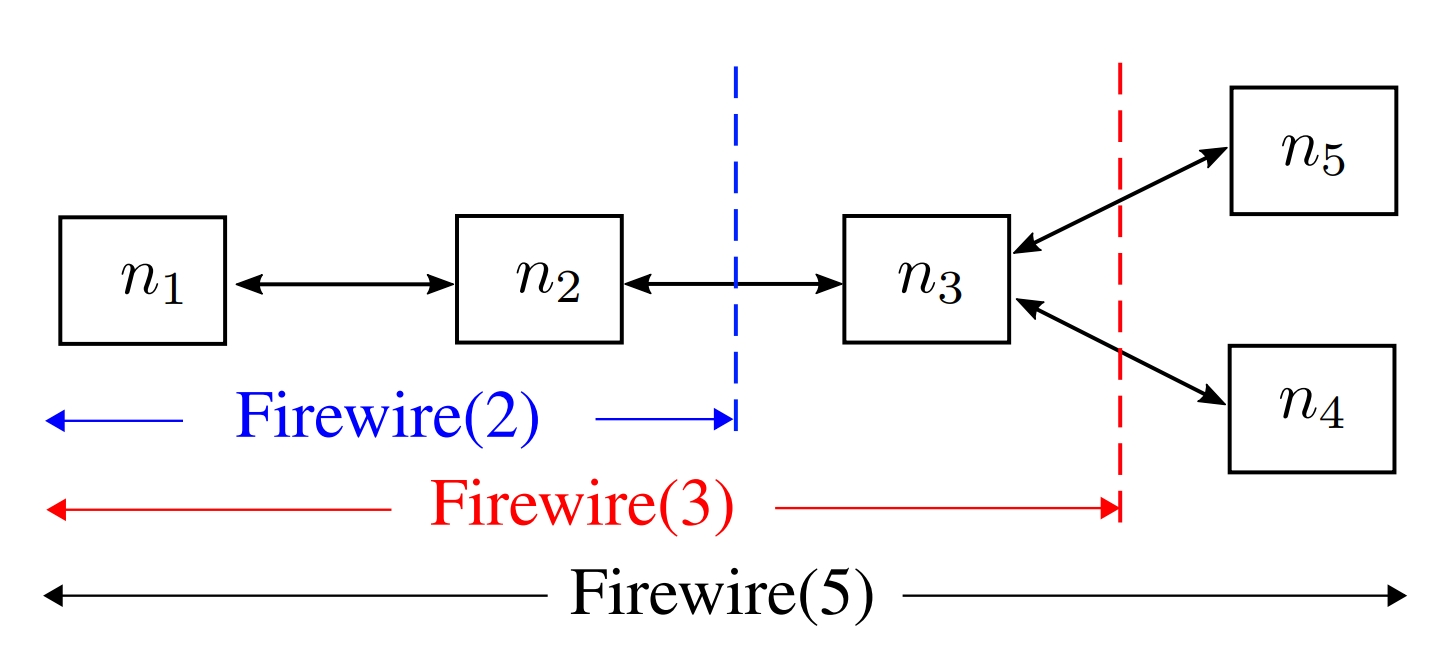
\includegraphics[scale=0.2]{Figures/firewireg}
\caption{FireWire Topologies with 2, 3 and 5 nodes}
\label{fig:fwg}
\end{figure}
The tree identification protocol is initiated by the leaf nodes of the topology. They send 
requests asking their neighbors to become their parents. A parent request sending mode is 
non deterministically chosen to be \emph{fast} or \emph{slow}. It determines the amount of time 
to wait before sending. Internal nodes of the topology keep on listening to parent requests 
until they receive exactly $n-1$ requests, $n$ being the number of neighbors. 
Then, they send a parent request
to their remaining neighbor. When receiving a parent request, a node either sends an 
acknowledgment, or detects a contention in the case it has also sent a parent request and it
is still waiting for an acknowledgment. Intuitively, a contention means that two neighbors are 
mutually asking to be leader. This situation is resolved by forcing both nodes to send new 
requests after a random waiting time.
We implemented a FireWire model inspired from the case-study in~\cite{firewire}, where the 
considered topology is made of two devices. 
Figure~\ref{fig:node} depicts the model for the node component.
\begin{figure}[!h]
 \centering
\begin{tikzpicture}[->,node distance=1.3cm,>=stealth',bend angle=20,auto,
  place/.style={circle,thick,draw=blue!75,fill=blue!20,minimum size=10mm},
  red place/.style={place,draw=red!75,fill=red!20}
  every label/.style={red},
  every node/.style={scale=.6},
  dots/.style={fill=black,circle,inner sep=2pt},
  initial text={}]

  \node [accepting, place,label=above:\textcolor{red}{$x\le 4$}] (l0)  {$\loc_0$};
  \node [place,below=1cm of l0,xshift=3cm,label=left:\textcolor{red}{$x\le 167$}] (l1) {$\loc_1$};
  \node [place,below=1cm of l0,xshift=-3cm,label=right:\textcolor{red}{$x\le 85$}] (l2) {$\loc_2$};
  \node [place,below=2.5cm of l0] (l3) {$\loc_3$};
  \node [place,below=1cm of l3, xshift=-3cm,label=below:\textcolor{red}{$x\le 4$}] (l4) {$\loc_4$};
  \node [place,below=1cm of l3,xshift=3cm] (l5) {$\loc_5$};
  \node [place,right=4cm of l3] (l6) {$\loc_6$};
  \node [place,left=4cm of l3] (l7) {$\loc_7$};
  
  
  \path (l0) edge node[sloped,midway,above]{$slow$} node[sloped,midway,below]{$x:=0$} (l1)
        (l0) edge node[sloped,midway,above]{$fast$}node[sloped,midway,below]{$x:=0$} (l2)
        (l1) edge node[sloped,midway,above]{$wait$}node[sloped,midway,below]{$159\le x\le167$} (l3)
        (l2) edge node[sloped,midway,above]{$wait$}node[sloped,midway,below]{$76\le x\le85$} (l3)
        (l2) edge [bend right] node[left,align=center]{$rcv\_req$\\$x:=0$} (l4)
        (l3) edge node[sloped,above, midway,align=center]{$rcv\_req$\\$x:=0$} (l4)
        (l3) edge node[sloped,above,midway,align=center]{$snd\_req$\\$x<=4$} (l5)
        (l5) edge[bend right=30] node[sloped,below,midway,align=center]{$rcv\_ack$} (l6)
        (l4) edge[bend left=30]node[sloped,below,midway]{$snd\_ack$} (l7);
        
        
  \draw[->] (l5) to[in=0,out=20,bend angle=30]node[sloped,above,midway]{$contention$} node[sloped,midway,below]{$x:=0$} (l0);
  \draw[->] (l6) to[in=10,out=90]node[sloped,above,midway]{$slave$}node[sloped,midway,below]{$x:=0$}  (l0);
  \draw[->] (l7) to[in=170,out=90]node[sloped,above,midway]{$leader$}node[sloped,midway,below]{$x:=0$}  (l0);
  \draw[->] (l1) to[bend left=25] node[sloped,above,midway,xshift=-1.2cm,yshift=2mm]{$rcv\_req$}node[sloped,midway,below,xshift=-1.2cm]{$x:=0$} (l4);
\end{tikzpicture}
  \caption{Timed Automaton for a Node}
 \label{fig:node}
\end{figure}  





\subsubsection{Gear Controller System}

The gear controller system (Figure~\ref{fig:gear}) describes the control system responsible 
for the gear change inside a
vehicle. The used model encompasses formal models of the gear controller and its environment.
The whole system includes five components: an interface, a controller, a clutch, an engine a
gear-box and two global variables. In order to change the gear, the interface sends a signal to 
the controller. Consequently, the controller interacts with the engine, the clutch and the 
gear-box to achieve the gear change. The engine is responsible of either regulating the torque 
or synchronizing the speed. On the other hand, the gear-box sets the gear between some fixed 
bounds, whereas, the clutch is used whenever the engine is not able to function properly 
(under difficult driving conditions, for instance). 
The case study was initially designed in UPPAAL~\cite{gear} and has been translated to BIP.
\begin{figure}[!h]
 \centering
\begin{tikzpicture}[
    dots/.style={fill=black,circle,inner sep=1pt},
  initial text={}]

\node (gc) [rectangle, draw=black, rounded corners, minimum width=30mm, minimum height=10mm] {Gear Controller};
\node (gb) [rectangle, draw=black, rounded corners, minimum width=30mm, minimum height=10mm,below=7.5mm of gc] {Gear Box};
\node (inf) [rectangle, draw=black, rounded corners, minimum width=30mm, minimum height=10mm,above=7.5mm of gc] {Interface};
\node (c) [rectangle, draw=black, rounded corners, minimum width=30mm, minimum height=10mm,below=7.5mm of gc, xshift=3.2cm] {Clutch};
\node (e) [rectangle, draw=black, rounded corners, minimum width=30mm, minimum height=10mm,below=7.5mm of gc, xshift=-3.2cm] {Engine};

  \node (i1) at ($(gc.north west)!0.7!(gc.north east)$) {};
  \node (i2) at ($(gc.north west)!0.3!(gc.north east)$) {};

  \node (i3) at ($(inf.south west)!0.7!(inf.south east)$) {};
  \node (i4) at ($(inf.south west)!0.3!(inf.south east)$) {};
  
  \draw[->] (i1.center) -- (i3.center);
  \draw[->] (i4.center) -- (i2.center);

  \node (i1) at ($(gb.north west)!0.7!(gb.north east)$) {};
  \node (i2) at ($(gb.north west)!0.3!(gb.north east)$) {};

  \node (i3) at ($(gc.south west)!0.7!(gc.south east)$) {};
  \node (i4) at ($(gc.south west)!0.3!(gc.south east)$) {};
  
  \draw[->] (i1.center) -- (i3.center);
  \draw[->] (i4.center) -- (i2.center);

  \node (i1) at ($(gc.north west)!0.7!(gc.south west)$) {};
  \node (i2) at ($(gc.north west)!0.3!(gc.south west)$) {};

  \node (i3) at ($(e.north west)!0.7!(e.north east)$) {};
  \node (i4) at ($(e.north west)!0.3!(e.north east)$) {};
  
  \draw[->] (i1.center) -| (i3.center);
  \draw[->] (i4.center) |- (i2.center);
  
  \node (i1) at ($(gc.north east)!0.7!(gc.south east)$) {};
  \node (i2) at ($(gc.north east)!0.3!(gc.south east)$) {};

  \node (i3) at ($(c.north west)!0.3!(c.north east)$) {};
  \node (i4) at ($(c.north west)!0.7!(c.north east)$) {};
  
  \draw[->] (i1.center) -| (i3.center);
  \draw[->] (i4.center) |- (i2.center);
\end{tikzpicture}
  \caption{Gear Controller System}
 \label{fig:gear}
\end{figure}  



The complete model (taken form~\cite{gear}) can be found in Appendix~\ref{ap1}.
\begin{remark}
Note that since the gear controller system contains to global variables, we had to tweak the 
generated invariants of the RTD-Finder tool as well as some of the predicates in order to 
restrict the set of reachable states of the system.
\end{remark}

\subsection{Results}
The experiments have been conducted on a HP machine with Ubuntu 16.04, an 
Intel\textsuperscript{\textregistered} Core\textsuperscript{\texttrademark}i5-4300U
processor of frequency 1.90GHz×4, and 7.7GiB memory.
\subsubsection{Conflict Detection Optimization}

\begin{table}[H]
  \caption{Experimental results}
    \label{tab:res}
  \begin{center}
\begin{tabular}{| l || c | c | c | c | c | c | c |}
    \hline
    Model                              & $n$                      & $i$                    & $c$          & $p$   & $f$   & $g$    & $t$   \\ \hline \hline                                  
    \multirow{14}{*}{Task Manager}     & 4                        & 8                      & 2            & 4     & 3     &  75\%  & 60.55ms \\ \cline{2-7}
                                       & \multirow{3}{*}{12}      & \multirow{3}{*}{40}    & 2            & 40    & 30    &  75\%  & 367.19ms \\ \cline{4-7}
                                       &                          &                        & 5            & 64    & 48    &  75\%  & 521.45ms \\ \cline{4-7}
                                       &                          &                        & 10           & 68    & 51    &  75\%  & 545.34ms \\ \cline{2-7}
                                       & \multirow{3}{*}{22}      & \multirow{3}{*}{80}    & 2            & 80    & 60    &  75\%  & 2.14s \\ \cline{4-7}
                                       &                          &                        & 10           & 144   & 108   &  75\%  & 3.41s \\ \cline{4-7}
                                       &                          &                        & 20           & 148   & 111   &  75\%  & 3.69s \\ \cline{2-7}
                                       & 32                       & 120                    & 30           & 228   & 171   &  75\%  & 8.41s \\ \cline{2-7}
                                       & 42                       & 160                    & 40           & 308   & 231   &  75\%  & 20.72s \\ \cline{2-7}
                                       & \multirow{6}{*}{52}      & \multirow{6}{*}{200}   & 2            & 200   & 150   &  75\%  & 22.56s \\ \cline{4-7}
                                       &                          &                        & 5            & 320   & 240   &  75\%  & 34.78s \\ \cline{4-7}
                                       &                          &                        & 10           & 360   & 270   &  75\%  & 37.72s \\ \cline{4-7}
                                       &                          &                        & 25           & 384   & 288   &  75\%  & 41.69s \\ \cline{4-7}
                                       &                          &                        & 50           & 388   & 291   &  75\%  & 45.35s \\ \cline{4-7}\hline
    \makecell{Train Gate\\Controller}  & 22                       & 45                     & 20           & 74    & 37    &  50\%  & 813,62ms \\ \hline
    \makecell{Gear \\Controller}       & 5                        & 32                     & 4            & 8     & 3     &  37.5\%  & 5,94s \\ \hline

  \end{tabular}
\end{center}
\end{table}
Table~\ref{tab:res} summarizes for each experiment the number of components ($n$), 
interactions ($i$),
partition classes ($c$), potential conflicts ($p$), false conflicts ($f$), the gain of the 
conflict detection 
and gives also the total verification time of our methods combined.
The above results give an indication on how much conflict resolution will be needed during 
execution. 

We first performed several experiments on different variants of the Task Manager example 
(with 2, 10, 20, 30, 40 and 50 Tasks). Each variant was tested with different partitioning of
interaction (different number of classes). Note that each time we chose the interaction
partition such that it yield the maximum number of potential conflicts. 
We can notice from the Task Manger experiments that increasing the number of interaction 
partition classes will increase the number of potential conflicts, that is,
the more distributed the system is the more conflicts it contains. 
Remark  that the percentage of gain remains the same meaning that our detection method
is not affected by the partitioning but rather bu the overall structure and dynamics of 
a given system.

We performed other experiments on real-life case studies such as the Train Gate Controller 
and the Gear Controller Systems which also yield interesting results in term of conflict 
detection ratio and execution time.

\subsubsection{Action-Time-Lock Detection for the \lpsabr}

Table~\ref{t:1} depicts the values $h_{\max}$ for each interaction of the Task Manager example, 
obtained while fixing $h_{\min}$.
Notice that the symmetry of the system implies the same $h_{\max}$ for interactions 
$\alpha_i,\alpha_{i+1},i\in\{1,3,5,7\}$. 
By remarking that location $\loc_3^2$ (resp. $\loc_3^3$) has a time progress condition 
$x\le4$ (resp. $y\le4$), and by observing that the clock $x$ is reset on the transition 
leading to this location, we can conclude that planning
the system with $h_{\min}>4$ will lead to an action-time-lock.
Particularly, in Example~\ref{exp:dl}, for $h_{\min}=2$ interaction $\alpha_6$ was planned 
with a horizon $\delta=8$, and consequently, leads to a action-time-lock state. Our method 
detects such cases and thus, finds that the maximum horizon for this interaction is 7. 
Likewise, the $h_{\max}$ for interactions $\alpha_2, \alpha_4\text{ and }\alpha_8$ 
(resp. $\alpha_1, \alpha_3\text{ and }\alpha_7$)
is found to be unbounded ($+\infty$).

\begin{table}[H]
  \caption{Detailed Results of the Task Manager Experiments}\label{t:1}
  \centering
  %  \vspace*{3mm}
  \begin{tabular}{| c || c | c | c | c |}
    \hline
    $h_{\min}$ & $\hmxb{\alpha_1}$, $\hmxb{\alpha_2}$ & $\hmxb{\alpha_3}$, $\hmxb{\alpha_4}$ & $\hmxb{\alpha_5}$, $\hmxb{\alpha_6}$  & $\hmxb{\alpha_7}$, $\hmxb{\alpha_8}$\\ \hline
        4      &                $+\infty$                    &                 $+\infty$                   &                9                     &               $+\infty$                 \\\hline
        3      &                $+\infty$                    &                 $+\infty$                   &                8                     &               $+\infty$                 \\\hline
        2      &                $+\infty$                    &                 $+\infty$                   &                7                     &               $+\infty$                 \\\hline
        1      &                $+\infty$                    &                 $+\infty$                   &                6                     &               $+\infty$                 \\\hline
  \end{tabular}
\end{table}

Table~\ref{t:2} summarizes the experiments obtained on the benchmarks stated above, where $n$ is
the number of components, $nb_{\I}$ the number of time progress conditions that will be 
verified
against action-time-lock freedom and
$\max h_{\min}$ the maximum value of $h_{\min}$ for which the system is action-time-lock-free in 
the planning semantics.
Additionally, the column $h_{\max}$ indicates whether a restriction on the upper horizons is 
required to avoid
deadlocks. Finally, $t_{exec}$ gives an overview of the execution time including both the 
invariants generation and the verification time.

\begin{table}[H]
  \caption{Experiments Results}\label{t:2}
 %   \vspace*{3mm}
  \centering
  \begin{tabular}{| c || c| c | c | c | c | c |}
  \hline
    Model                              & $n$ & $nb_{\I}$&  $\max h_{\min}$ &   $h_{\max}$ & $t_{exec}(s)$ \\\hline 
    Task Manager                       & 4  & 4  & 4            &  B         & 0.11 \\\hline 
    Train Gate Controller              & 3  & 6  & 4            &  $+\infty$        & 0.16   \\\hline 
    Firewire                           & 4  & 10 & 5            &  $+\infty$        & 3.03   \\\hline 
    Gear Controller                     & 5  & 19 & 130          &  $+\infty$        & 4.65    \\\hline 
  \end{tabular}
\end{table}

As shown in table~\ref{t:1}, the task manager model has a maximal $\hmin$ value of 4 TU 
and requires a restriction
on the upper horizons for interactions $\alpha_5$ and $\alpha_6$.
In the same way, we found that the train gate controller, the firewire and the train gate 
controller models have respectively maximal $\hmin$ value 
of 4 TU, 5 TU and 130 TU. However, they do not require any restriction on the upper 
horizons values of their interactions.





%\chapter{Experimental Results}
\label{chap:8}
\minitoc
\section{Case Studies}


\part{Conclusion}
{\label{part:3}}
%\chapter{Conclusion and Perspectives}
\label{chap:9}
\minitoc

\listoffigures 

\listoftables 


% ********************************** Back Matter *******************************
% Backmatter should be commented out, if you are using appendices after References
%\backmatter

% ********************************** Bibliography ******************************
\begin{spacing}{0.9}

% To use the conventional natbib style referencing
% Bibliography style previews: http://nodonn.tipido.net/bibstyle.php
% Reference styles: http://sites.stat.psu.edu/~surajit/present/bib.htm

\bibliographystyle{alpha}
\cleardoublepage
\bibliography{References/references} % Path to your References.bib file


% If you would like to use BibLaTeX for your references, pass `custombib' as
% an option in the document class. The location of 'reference.bib' should be
% specified in the preamble.tex file in the custombib section.
% Comment out the lines related to natbib above and uncomment the following line.
%\printbibliography[heading=bibintoc, title={References}]


\end{spacing}

% ********************************** Appendices ********************************

\begin{appendices} % Using appendices environment for more functunality

\chapter{The Gear Controller System}
\label{ap1}


\begin{figure}[H]       
\centering            
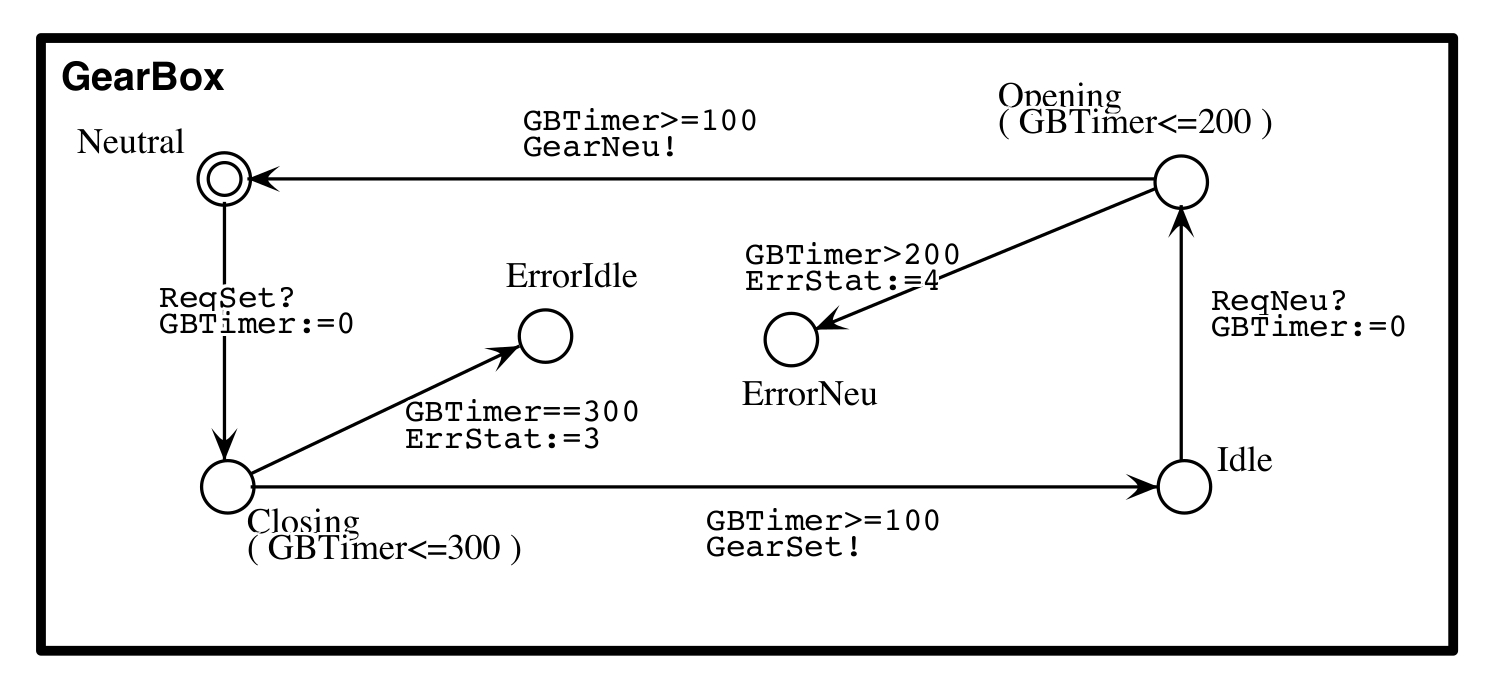
\includegraphics[scale=0.25]{Figures/gbgb}
\caption{The Gearbox Component}
\label{fig:gbgb}         
\end{figure}  


\begin{figure}[H]       
\centering            
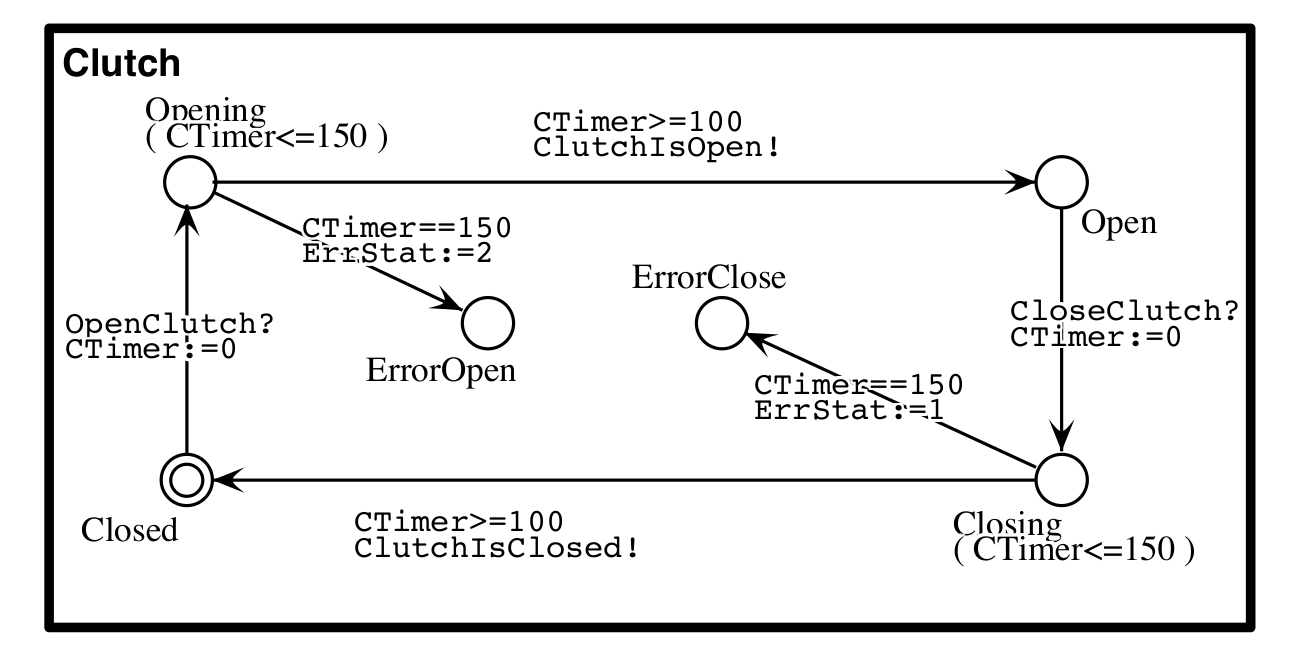
\includegraphics[scale=0.29]{Figures/gbc}
\caption{The Clutch Component}
\label{fig:gbc}         
\end{figure}  

\begin{figure}[H]       
\centering            
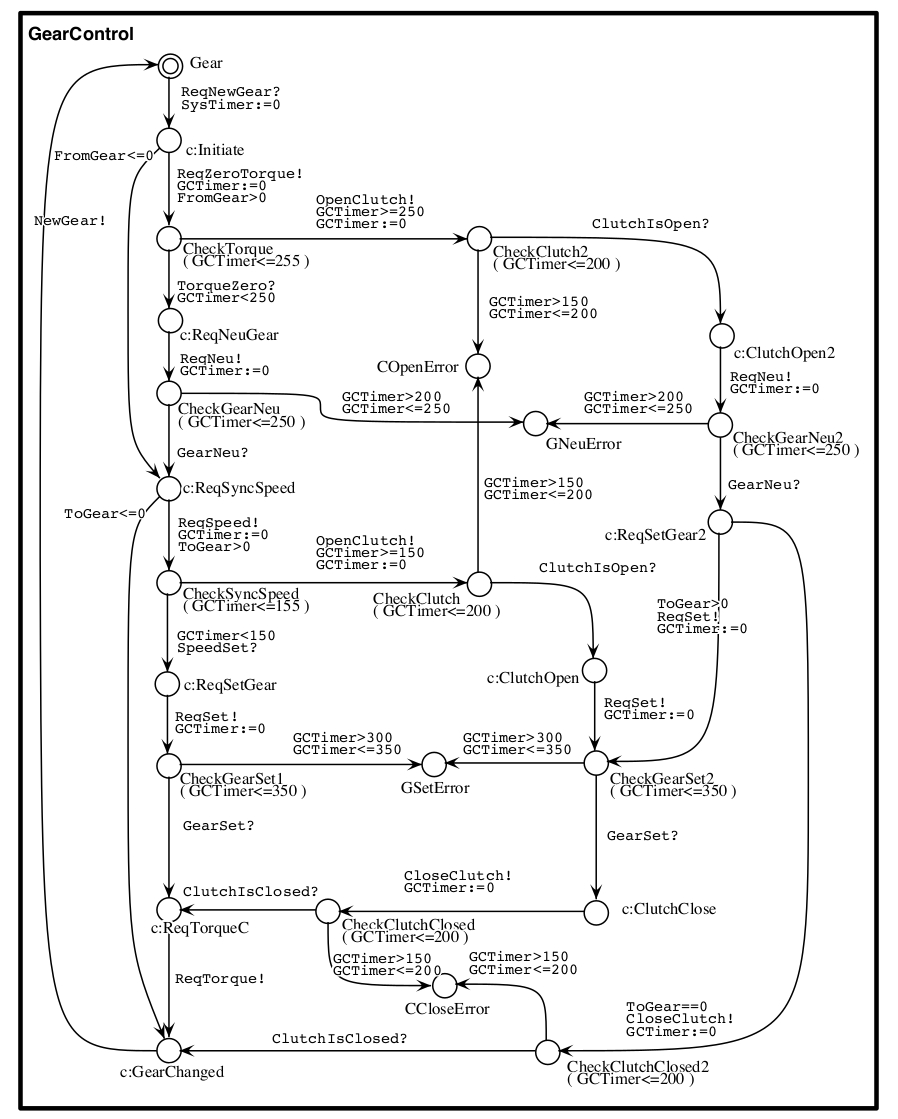
\includegraphics[scale=.55]{Figures/gbgc}
\caption{The Gearbox Controller Component}
\label{fig:gbgc}         
\end{figure}  

\begin{figure}[H]       
\centering            
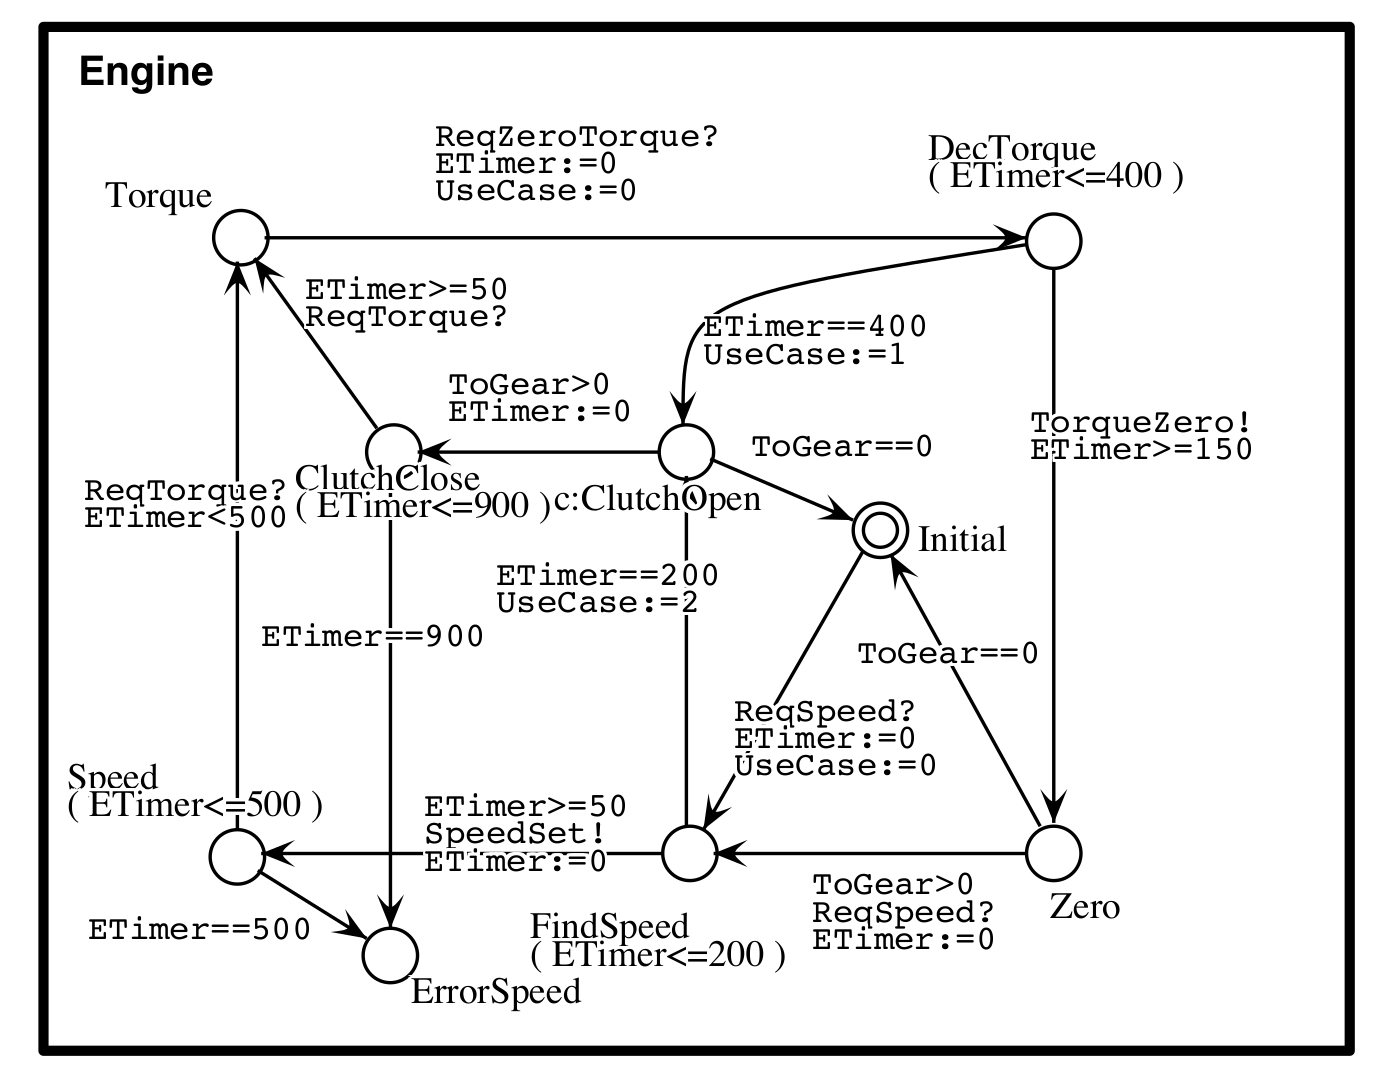
\includegraphics[scale=0.3]{Figures/gbe}
\caption{The Engine Component}
\label{fig:gbe}         
\end{figure}  

\begin{figure}[H]       
\centering            
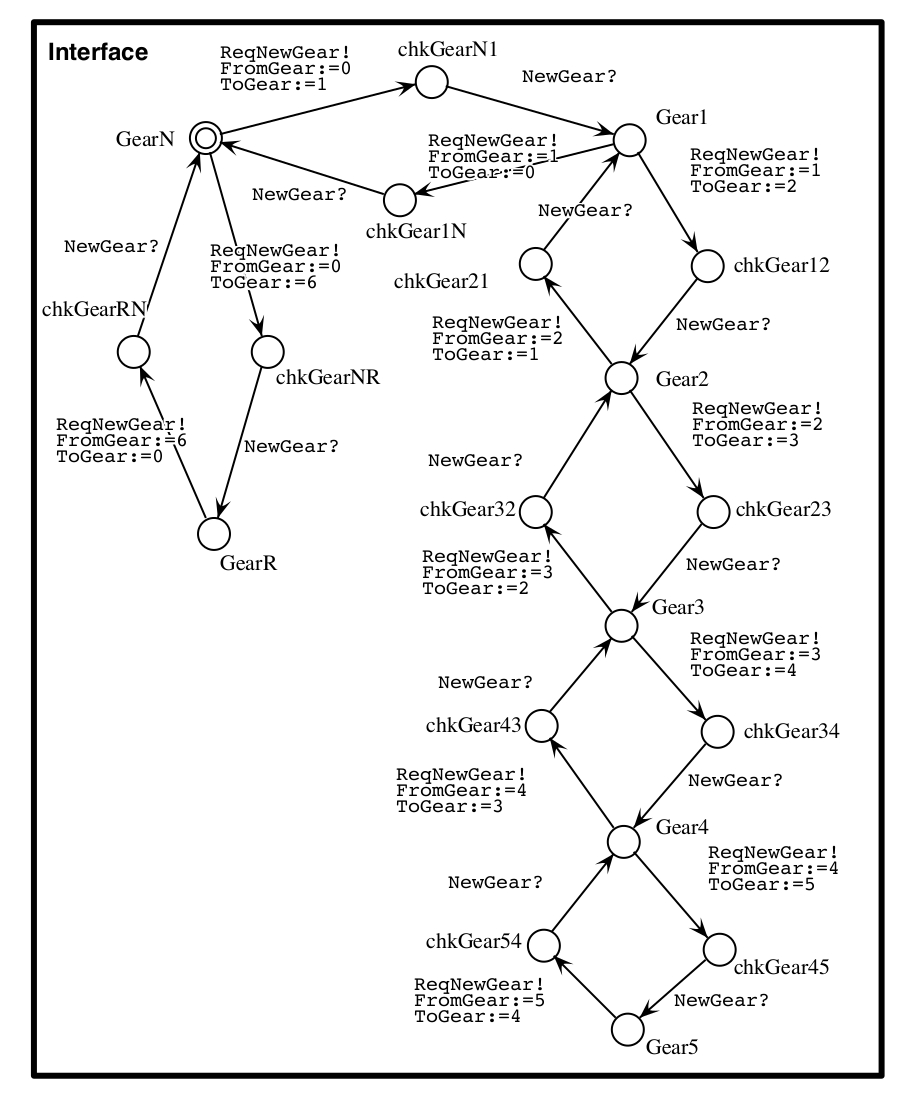
\includegraphics[scale=0.5]{Figures/gbi}
\caption{The Interface Component}
\label{fig:gbi}         
\end{figure}  


%\include{Appendix2/appendix2}

\end{appendices}

% *************************************** Index ********************************
\printthesisindex % If index is present

\end{document}
